%% -*- coding:utf-8 -*-
%% -*- coding:utf-8 -*-
%%%%%%%%%%%%%%%%%%%%%%%%%%%%%%%%%%%%%%%%%%%%%%%%%%%%%%%%%
%%   $RCSfile: hpsg-handout.tex,v $
%%  $Revision: 1.3 $
%%      $Date: 2006/05/17 12:19:27 $
%%     Author: Stefan Mueller (DFKI)
%%    Purpose: 
%%   Language: LaTeX
%%%%%%%%%%%%%%%%%%%%%%%%%%%%%%%%%%%%%%%%%%%%%%%%%%%%%%%%%
%% $Log: hpsg-handout.tex,v $
%% Revision 1.3  2006/05/17 12:19:27  stefan
%% *** empty log message ***
%%
%% Revision 1.2  2004/08/14 15:44:44  stefan
%% konstituentenreihenfolge
%%
%% Revision 1.1  2004/06/21 19:14:48  stefan
%% alte Version vor LaTeX-Beamer
%%
%% Revision 1.1  2002/01/09 20:06:23  stefan
%% Initial revision
%%
%% Revision 1.1  2001/10/21 17:01:35  stefan
%% Initial revision
%%
%%%%%%%%%%%%%%%%%%%%%%%%%%%%%%%%%%%%%%%%%%%%%%%%%%%%%%%%%

\documentclass[xcolor=dvipsnames,blackandwhite,slidestop,handout,10pt]{beamer}

%% -*- coding:utf-8 -*-


\usepackage{styles/Beamer/hu-beamer-includes-pdflatex} %,beamer-movement}


% no book icon please
\setbeamertemplate{bibliography item}{}

% Checkmark
%\usepackage{tikz} % Examples and documentation: http://www.texample.net/tikz
%\usepackage{bbding}
\makeatletter
\newcommand{\dingfamily}{\fontencoding{U}\fontfamily{ding}\selectfont}
\newcommand{\@chooseSymbol}[1]{{\dingfamily\symbol{#1}}}
\newcommand{\Checkmark}{\@chooseSymbol{'041}}
\makeatother

%\fuberlinlogon{0.89cm}

% creates an unggly bibliography
%\usepackage[T1]{fontenc}


\usepackage{jambox}

\usepackage{epsfig}
\usepackage{tabularx}

%\usepackage{tikz-grid}

%\renewcommand{\trace}{\raisebox{0.2ex}{\_}\rule{0cm}{0.7em}}


%\usepackage[T4,T1]{fontenc}

% die machen \! kaputt
%\usepackage{tipa,tipx,phonetic}

% \TH, \th, \dh, \DH
\usepackage{wasysym}

\let\TH=\Thorn
\let\th=\thorn

% Das ʒ muss aus tipa.sty muss auf textyogh umgebogen werden, da war \textezh drin.


\let\textezh=\textyogh
\let\textoopen=\textopeno
%\let\texteopen=\textopene gibts nicht
\let\texteopen=\textepsilon
\let\textgammalatinsmall=\textbabygamma
\let\ng=\engma
\let\textvhook=\textscriptv

%\DeclareUnicodeCharacter {720}{\textlengthmark }
%\DeclareUnicodeCharacter {635}{\textturnrrtail\,}

%% \nodemargin5pt%\treelinewidth2pt\arrowwidth6pt\arrowlength10pt
%% \selectlanguage{german}
%% \psset{nodesep=5pt} %,linewidth=0.8pt,arrowscale=2}
%% \psset{linewidth=0.5pt}

\usepackage[customcolors]{hf-tikz}

% for subnodes in trees
% is in hu-beamer-...
%% \usepackage{tcolorbox}
%% \tcbuselibrary{skins}
%% \newtcbox{\mybox}[1][]{empty,shrink tight,nobeforeafter,on line,before upper=\vphantom{gM},remember as=#1,top=2pt,bottom=2pt}


%\beamertemplateemptyfootbar

%\hypersetup{pdfauthor={Stefan Müller (unter Benutzung von Material von Peter Gallmann, FSU Jena)}}
%\hypersetup{pdftitle={Head-Driven Phrase Structure Grammar für das Deutsche}}


%\subject{Generative Grammatik für das Deutsche}


%\beamerdefaultoverlayspecification{<+->}

\let\mc=\multicolumn


\newcommand{\sigle}[1]{\tiny{#1}}



%\mode<beamer>{\beamertemplatebackfindforwardnavigationsymbolshorizontal}




\title{Strukturen der germanischen Sprachen}

%\includeonly{organisatorisches-germanisch-vl}
%\includeonly{germanisch-phaenomene}
%\includeonly{germanisch-valenz-scrambling}
%\includeonly{germanisch-verbalkomplex}
%\includeonly{germanisch-verbstellung}
%\includeonly{germanisch-extraction}
%\includeonly{germanisch-mehr-vf}
%\includeonly{germanisch-subjekt}
%\includeonly{germanisch-passiv}
%\includeonly{germanisch-expletives}

\begin{document} 
\hypersetup{bookmarksopen=false}

\exewidth{(35)}

%%% -*- coding:utf-8 -*-
\section{Organisatorisches}

\frame{
\frametitle{Organisatorisches}


\begin{itemize}
%% \item alle Teilnehmer bitte Mail in Maillisten eintragen\\
%%       zugänglich von \url{http://www.cl.uni-bremen.de/~stefan/Lehre/HPSG/}
%%   \begin{itemize}
%%   \item Mail-Liste für alle Linguistik-Studierenden
%%   \item Mail-Liste für alle Teilnehmer dieser Veranstaltung
%%   \end{itemize}
\item Bitte bei moodle anmelden (gibt kein Passwort)
\pause
\item Telefon und Sprechzeiten siehe: \url{https://hpsg.hu-berlin.de/~stefan/}
\pause
\item Beschwerden, Verbesserungsvorschläge:
      \begin{itemize}
      \item mündlich
      \item per Mail oder 
      \item anonym über das Web:\\
            \url{https://hpsg.hu-berlin.de/~stefan/Lehre/}
      \end{itemize}
\item Bitte unbedingt Mail-Regeln beachten!\\
\url{https://hpsg.hu-berlin.de/~stefan/Lehre/mailregeln.html}
\end{itemize}
}

\frame{
\frametitle{Materialien}


\begin{itemize}

\item Information zur Vorlesung:\\
\url{https://hpsg.hu-berlin.de/~stefan/Lehre/Germanisch/}

\item Wiederholung/Grundlagen: \citew[Kapitel~1--2]{MuellerGTBuch2}
\item Einführungsbuch zur HPSG: \citew{MuellerLehrbuch3}
    
\end{itemize}
}

\frame{
\frametitle{Vorgehen}


\begin{itemize}
\item Handouts ausdrucken, immer mitbringen und persönliche Anmerkungen einarbeiten
\item Veranstaltungen vorbereiten
\item Veranstaltungen unbedingt nacharbeiten!
      \begin{itemize}
      \item Kontrollfragen
      \item Übungsaufgaben
      \end{itemize}
\item Fragen!
\end{itemize}
}


\section{Leistungen}
\frame{
\frametitle{Leistungen}

BA Ling: Modul 3: Grammatik II: Der Satz\\
BA Deutsch: Modul 6 Wort und Satz

\begin{itemize}
      \item Studiengang BA Germanistische Linguistik: Klausur in der letzten Woche im Vorlesungsraum
        bzw. dann im zweiten Prüfungszeitraum
      \item für alle (freiwillig): 
        \begin{itemize}
        \item kleine Tests zur Vertiefung
        \item zwei Fragen zum zu lesenden Text
        \end{itemize}
%Hausarbeit (\url{https://hpsg.hu-berlin.de/~stefan/Lehre/hausarbeiten.html})
\end{itemize}

Ideale Zeitaufteilung:

\begin{tabular}{@{}lr@{~}l}
Präsenzstudium Vorlesung  & 25 h \\
Vor- und Nachbereitung    & 35 h & (35/15 = 2 h 20 min für jede Sitzung)\\

Klausurvorbereitung       & 90 h & (90h/15 = 6h)
\end{tabular}

Das Modul entspricht 9 bzw.\ 8 Leistungspunkten.


}


%\input ../../plagiat.tex

\section{Ziele der Veranstaltung}


\frame{
\frametitle{Ziele}


% \begin{itemize}[<+->]
% \item Vermittlung grundlegender Vorstellungen über Grammatik
% \item Vorstellung zweier Grammatiktheorien und deren Herangehensweisen
% \item Vergleich der Sprachen Deutsch, Dänisch, Niederländisch
% \end{itemize}

\begin{itemize}
\item Überblick über die germanischen Sprachen
\item Detailliertere sprachvergleichende Diskussion ausgewählter syntaktischer Phänomene
\end{itemize}

Lehramtsrelevante Teilziele
\begin{itemize}
\item Wiederholung und Festigung grundlegender Begriffe:

\begin{itemize}
\item Wortarten
\item Kasus und andere morphosyntaktische Merkmale
\item Grammatische Funktionen
\item syntaktische Struktur des Deutschen und der Nachbarsprachen
      
      Hauptsätze/Nebensätze/Fragen

\item Valenz (Unterscheidung Argument/Adjunkt)
\item Aktiv/Passiv
\end{itemize}
\item Ansonsten: Blick über den Schul-Tellerrand
\end{itemize}


}

%\author{Matthias Hüning}\institute[FU Berlin, Philosophie und Geisteswissenschaften, Niederlandistik]{}

\subtitle{Überblick über die germanischen Sprachen}

\section{Überblick über die germanischen Sprachen}

\huberlintitlepage[22pt]


\outline{

\begin{itemize}
\item {Überblick über die germanischen Sprachen}
\item Phänomene
\item Phrasenstrukturgrammatiken und \xbart
\item Valenz, Argumentanordnung und Adjunkte
\item Verbalkomplexbildung in den SOV-Sprachen
\item Verbstellung: Verberst- und Verbzweitstellung
\item Passiv
\item Eingebettete Sätze
\end{itemize}

}

\frame{
\frametitle{Literaturhinweis}



Zu diesem Abschnitt gibt es das Kapitel~1 in \citew{MuellerGermanic}.


\begin{refsection}

\nocite{MuellerGermanic}

\printbibliography[heading=none,notkeyword=this]

\end{refsection}



}


%\part{Allgemeines}


\subsection{Sprachen und Sprecher*innen}

\frame{
\frametitle{Allgemeines: Sprachen und Sprecher*innen}


\begin{itemize}
\item ca.\ 5000 bis 6000 Sprachen auf der Welt
\pause
\item Germanische Sprachen bilden eine kleine Gruppe\\
(je nach Zählung etwa 15 Sprachen)
\pause
\item Problem: Abgrenzung von Sprache und Sprachvarietät\\
      (\zb Varietäten des Friesischen)\\
"`Eine Sprache ist ein Dialekt mit einer Armee und Flotte."' (Max Weinreich)
\pause
\item insgesamt fast 500 Millionen Sprecher*innen (Muttersprachler)\\
      $>$ 1/12 der Weltbevölkerung
\pause
\item große regionale Verbreitung (insbesondere Englisch)

\end{itemize}

}


\subsection{Gängige Einteilung}

\frame{
\frametitle{Gängige Einteilung}

\begin{itemize}
\item Ostgermanisch\\
Gotisch (ausgestorben)
\pause
\item Westgermanisch\\
Deutsch, Jiddisch, Luxemburgisch, Pennsylvanisch,
Plautdietsch, Niederländisch, Afrikaans, Friesisch, Englisch
\pause
\item Nordgermanisch\\
Dänisch, Schwedisch, Norwegisch, Isländisch, Färöisch
\end{itemize}


}

\subsection{Historische Bemerkungen}

\frame{
\begin{itemize}
\item Germanisch: selbständiger Zweig in der indoeuropäischen Sprachfamilie
\pause
\item Zwischen 2000 und 1000 v.\,Chr. Ausgliederung des Proto-Germanischen aus dem indoeuropäischen Sprachkontinuum
\pause
\item Ursprünge in der baltischen Region (Norddeutschland,
Südskandinavien); Ausbreitung von Nordsee bis Polen (ca.\,500
v.\,Chr.)
\pause
\item Veränderungen im Konsonantismus\\
      (Erste bzw. Germanische Lautverschiebung; bis ca.\ 2.\,Jh.\,v.\,Chr.)
\pause
\item Erste schriftliche Zeugnisse:\\
      Runeninschriften (ab ca.\ 300 n.\,Chr.; gotische Bibelübersetzung im 4.\,Jh.)
\end{itemize}

}


\subsection{Die indoeuropäische Sprachfamilie}


\frame{

\includegraphics[width=70mm]{Bilder/indoeuropaeisch}
aus \citew[S.\,665]{Fitch2007a-u}

}

\subsection{Verwandschaft}

\frame{
Lautliche Übereinstimmung bei Worten aus dem zentralen
Wortschatz

\oneline{%
\begin{tabular}{lllllllll}
Niederländisch & vader  & vier    & vol    & huis  & bruin  & uit & kruid     & muis\\
Deutsch        & Vater  & vier    & voll   & Haus  & braun  & aus & Kraut     & Maus\\
Englisch       & father & four    & full   & house & brown  & out & crowd (?) & mouse\\
Friesisch      & –      & fjouwer & fol    & hûs   & brún   & út  & krûd      & mûs\\
Schwedisch     & fader  & fyra    & full   & hus   & brun   & ut  & krut      & mus\\
Dänisch        & fader  & fire    & fuld   & hus   & brun   & ud  & krudt     & mus\\
Norwegisch     & far    & fire    & full   & hus   & brun   & ut  & krydder   & mus\\
Isländisch     & faðir  & fjórir  & fullur & hús   & brúnn  & út  & –         & mús\\
\end{tabular}
}

}

\subsection{Entwicklung der germanischen Sprachen}

\frame{
\frametitle{Entwicklung der germanischen Sprachen}


%\includegraphics[width=\textwidth]{Bilder/stammbaum-germanisch}
%aus \citew[S.\,251]{Bussmann2002a}


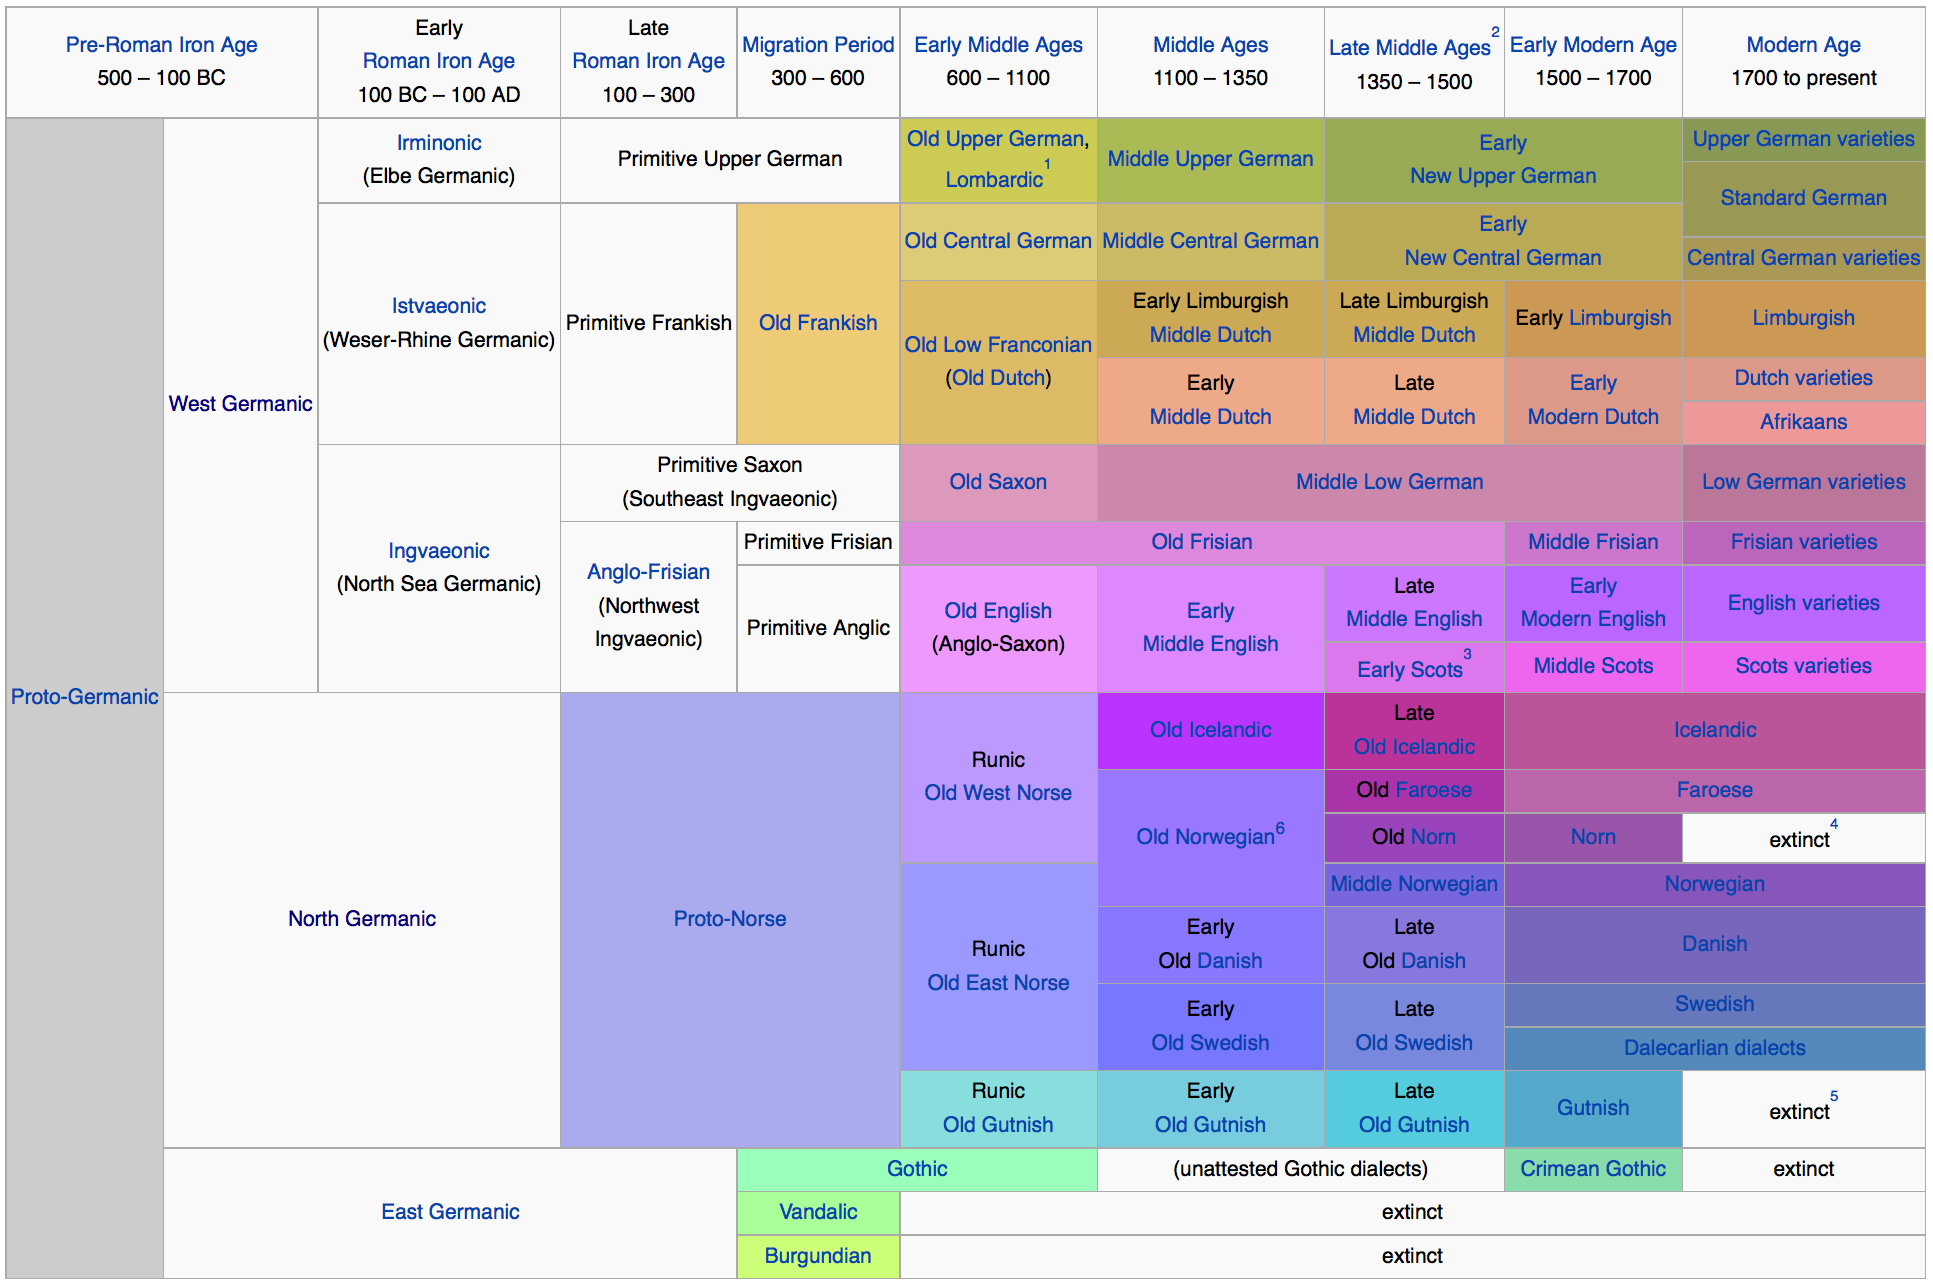
\includegraphics[width=.75\textwidth]{Bilder/germanic-wikipedia}

\oneline{Quelle: Englische Wikipedia: \url{https://en.wikipedia.org/wiki/Germanic_languages\#Diachronic}}


}



\subsection{Drei Zweige des Germanischen}

\frame{
\frametitle{Drei Zweige des Germanischen}

\begin{itemize}
\item Aufteilung des Protogermanischen in drei Zweige:\\
Ost-, West- und Nordgermanisch (etwa im ersten Jh.\ nach Chr.)
\pause

\item Ursachen:
\begin{itemize}
\item inhärente sprachliche Variation (Dialekte)
\item Migration (Sprachkontakt)
\item Standardisierung
\end{itemize}

\pause

\item Wir behandeln die Struktur germanischer Standardsprachen
\end{itemize}

}

\subsubsection{Ostgermanisch}

\frame{
\frametitle{Ostgermanisch}

\begin{itemize}
\item
ca.\ 100 v. Chr: Goten emigrieren von den dänischen Inseln
und aus Südschweden und treffen auf Vandalen und andere
Stämme
\pause
\item Sie konstituieren den ostgermanischen Zweig,\\ von dem nur
das Gotische überliefert ist
\pause
\item Mit dem Ende der Gotenreiche ist auch das Gotische
ausgestorben\\
(letzte Reste bis ca.\ 1800 auf der Halbinsel Krim)
\pause
\item Im 4.\ Jahrhundert übersetzte der westgotische Bischof
Wulfila die Bibel ins Gotische (Wulfila-Bibel)
\pause
\item  Bekannt ist vor allem das Manuskriptfragment in der
Universitätsbibliothek von Uppsala (Codex Argenteus)
\end{itemize}


}


\frame{
\frametitle{Wulfila-Bibel (Codex Argenteus)}

\begin{columns}[T]
\begin{column}{53mm}

\includegraphics[width=53mm]{Bilder/Wulfila_bibel}
\end{column}
\begin{column}{65mm}

Quelle: Wikipedia\\
\url{http://de.wikipedia.org/wiki/Bild:Wulfila_bibel.jpg}
\end{column}
\end{columns}

}

\subsubsection{Nordgermanisch}

\frame{
\frametitle{Nordgermanisch}

\begin{itemize}
\item erste Runen-Inschriften aus dem 6.\,Jh.
\item Sprache der Wikinger (800--1050) war noch relativ homogen
\item erst gegen Ende der Wikinger-Ära entstanden zwei Zweige:\\
 Ost-Skandinavisch (Altdänisch, Altschwedisch),\\
 West-Skandinavisch (Altnorwegisch, Altisländisch)
\end{itemize}

}



\subsubsubsection{Dänisch}

\frame{
\frametitle{Dänisch}

\begin{itemize}
\item Dänisch (dansk): offizielle Sprache des Königreichs Dänemark,
zweite Amtssprache der Färöer-Inseln und Grönlands (Inuit als
erste Sprache)
\item ca.\ 5,5 Millionen Sprecher*innen
\item ca.\ 50.000 Sprecher*innen in Schleswig Holstein
\item das Dänische hat sich von allen skandinavischen Sprachen am
weitesten von den gemeinskandinavischen Wurzeln entfernt
\end{itemize}

}



\subsubsubsection{Schwedisch}

\frame{
\frametitle{Schwedisch}

\begin{itemize}
\item Schwedisch (svenska):\\
offizielle Sprache in Schweden mit ca.\ 8,5 Millionen Muttersprachlern
\item erste Sprache von ca.\ 300.000 Sprecher*innenn in Finnland
\item Bis zur Wikingerzeit sind Dänisch und Schwedisch kaum
voneinander zu unterscheiden; 

ab ca.\ 800 entwickeln sie sich auseinander; 

seit ca.\ 1300 deutlich unterscheidbar
\end{itemize}

}


\subsubsubsection{Isländisch}

\frame{
\frametitle{Isländisch}

\begin{itemize}
\item Isländisch (íslenska) ist die westskandinavische Sprache Islands
seit der Besiedlung vor über 1000 Jahren
\item ca.\ 260.000 Sprecher*innen
\item kaum Variation (keine Dialekte)
\item Konservativ: von allen skandinavischen Sprachen hat das
Isländische die Flexion und seinen germanischen Erbwortschatz
am besten bewahrt.
\item Zunächst kaum Unterschiede zum Norwegischen,\\
dann auseinander entwickelt
\end{itemize}

}



\subsubsubsection{Norwegisch}


\frame{
\frametitle{Norwegisch}

\begin{itemize}
\item Norwegisch (norsk) kennt zwei Varietäten:\\
Dänisch-Norwegisch (bokmål) und Neu-Norwegisch (nynorsk). 

Beide sind offizielle Landessprachen und werden nebeneinander verwendet.
\item Insgesamt ca.\ 4,3 Millionen Sprecher*innen.
\item Von 1380--1814 war Dänisch die Schriftsprache;\\
gesprochen wurden lokale Dialekte
\item norwegischer Standard musste daher erst geschaffen werden;\\
Ivar Aasen (1813--1896): nynorsk; offiziell anerkannt 1885
\item bokmål (`Buchsprache') ist die erste Sprache der Mehrheit
\end{itemize}

}




\subsubsubsection{Färöisch}

\frame{
\frametitle{Färöisch}

\begin{itemize}
\item Färöisch oder Färingisch (føroyskt) ist, zusammen mit Dänisch,\\
die offizielle Sprache der Färöer-Inseln
\item 47.000 Sprecher*innen
\item Färöer-Inseln gehören seit 1816 zu Dänemark, \\
seit 1948 Status eines autonomen Landesteils
\item Färöisch ist stark vom Dänischen beeinflusst
\item Schriftsprachliche Überlieferung erst seit 1773 und auch dann nur spärlich\\
(dies im Gegensatz zum Isländischen)
\end{itemize}

}




\subsubsection{Westgermanisch}

\frame{
\frametitle{Westgermanisch}

\begin{itemize}
\item kein homogener Ursprung, sondern drei Zweige von
Dialektgruppen (Nordseegermanisch, Weser-Rheingermanisch,
Elbgermanisch)
\item aber keine 1-zu-1-Zuordnung dieser Dialektgruppen zu den
heutigen Standardsprachen
\end{itemize}

}




\subsubsubsection{Deutsch}

\author{Matthias Hüning, Stefan Müller}\institute[FU Berlin, Philosophie und Geisteswissenschaften]{}

\frame{
\frametitle{Deutsch}


\begin{itemize}
\item Deutsch ist offizielle Landessprache von 
\begin{itemize}
\item Deutschland (ca.\ 80 Millionen Sprecher*innen), 
\item Österreich (7,5 Millionen), 
\item Liechtenstein
(15.000), 
\item Schweiz (4,2 Millionen, von insgesamt 6,4 Millionen
Schweizern), 
\item Italien/Südtirol (270.000), 
\item Belgien (65.000),
\item Luxemburg (360.000).
\end{itemize}
\item In Luxemburg gilt neben dem nicht-ursprünglichen Deutsch auch
das ursprüngliche Lëtzebuergesch als offizielle Sprache.
\item Insgesamt hat das Deutsche ca.\ 97 Millionen Sprecher*innen, davon
ca.\ 90 Millionen Muttersprachler und 7 Millionen
Zweitsprachler (täglicher Gebrauch)
% = Migrationshintergrund
% Quelle Wikipedia 15.10.2013


\item ca.\ 80 Mio Fremdsprachler, davon ca. 55 Mio in der EU
\end{itemize}

}




\author{Matthias Hüning}\institute[FU Berlin, Philosophie und Geisteswissenschaften, Niederlandistik]{}


\frame{
\frametitle{Deutsch}

\begin{itemize}
\item Drei nationale Hauptvarianten (Deutschland, Österreich, Schweiz);\\
in anderen Staaten meist Minderheitensprache
\item Zwei Dialektgruppen: Niederdeutsch/Plattdeutsch und
Hochdeutsch
\end{itemize}

}



\subsubsubsection{Jiddisch}

\frame{
\frametitle{Jiddisch}

\begin{itemize}
\item Jiddisch ist eine von vielen jüdischen Sprachen.\\
heute von ca.\ 2 Millionen Menschen in verschiedenen Regionen der Welt gesprochen,\\
davon die meisten in den USA (1,25 Mill.)
\item Vor 100 Jahren lebten weit über 7 Millionen Sprecher*innen des
Jiddischen in Europa, die meisten in Russland und in Österreich-Ungarn.
\item Heute höchstens noch 75.000 Jiddisch-Sprachige in Westeuropa
\item Ursprung: mittelalterliches Deutsch, vermischt mit Hebräisch und
Aramäisch
\end{itemize}

}


\subsubsubsection{Pennsylvania German}

\frame{
\frametitle{Pennsylvania German}

\begin{itemize}
\item Pennsylvanisch (Deitsch, auch bekannt als Pennsylvanian Dutch)
hat ca.\ 300.000 Muttersprachler, vor allem in den USA
\item Sprachinseln, vor allem in Pennsylvania, Ohio und Indiana
\item Auswanderung im 17. und 18. Jahrhundert; Mitglieder
verschiedener protestantischer Glaubensrichtungen (Mennoniten,
Pietisten usw.)
\item Sprache baut hauptsächlich auf Pfälzer Dialekten auf
\item heute vor allem gesprochen von Amischen und Mennoniten
\end{itemize}

}



\subsubsubsection{Niederländisch}

\frame{
\frametitle{Niederländisch}

\begin{itemize}
\item Niederländisch (Nederlands) ist offizielle Landessprache in den Niederlanden\\
(ca.\ 15 Millionen Sprecher*innen),\\
eine der Landessprachen in Belgien (ca.\ 6 Millionen; knapp 4 Millionen
Wallonen).
\item Es ist die offizielle Verwaltungs- und Unterrichtssprache in Surinam\\
 (seit 1975 unabhängig) und auf Aruba und den niederländischen Antillen
\end{itemize}

}



\subsubsubsection{Afrikaans}

\frame{
\frametitle{Afrikaans}

\begin{itemize}
\item Afrikaans ist eine der offiziellen Sprachen Südafrikas\\
      (insgesamt über 10 Amtssprachen)
\item ca.\ 6,4 Millionen Muttersprachler,
davon 6,2 Millionen in Südafrika\\ (= ca.\ 15\,\% der Bevölkerung) und 150.000 in Namibia
\item seit Mitte des 17.\ Jh.; Entwicklung aus niederländischen Dialekten;\\
Afrikaans wird seit dem frühen 19.\ Jh. als
eigenständige Sprache gesehen
\item Sprachkontakt; heute starker Einfluss des Englischen
\item starke Tendenzen zu struktureller Vereinfachung im
Sprachsystem
\end{itemize}

}



\subsubsubsection{Friesisch}

\frame{
\frametitle{Friesisch}

Drei Varietäten, untereinander nicht verständlich:\begin{itemize}
\item Nordfriesisch, ca.\ 10.000 Sprecher*innen, vor allem auf den
nordfriesischen Inseln (Amrum, Sylt, Helgoland)
\item Ostfriesisch, in Ostfriesland ausgestorben.\\
Überbleibsel: das Saterfriesische (wird in der Gemeinde Saterland im Landkreis
Cloppenburg von etwa 1.000 bis 2.500 Menschen
gesprochen)
\item Westfriesisch, niederländische Provinz Friesland,\\
 ca.\ 350.000 Muttersprachler
\end{itemize}


}



\subsubsubsection{Englisch}

\frame{
\frametitle{Englisch}

\begin{itemize}
\item Englisch hat gegen Ende des 20.\ Jh. ca.\ 570 Millionen Sprecher*innen in
aller Welt (337 Mill. Muttersprachler, 235 Mill. Zweitsprachler)
\begin{itemize}
\item USA: 227 Mill. Muttersprachler; 
\item Großbritannien: 57 Mill.;
\item Nigeria: 43 Mill.; 
\item Kanada: 24 Mill.; 
\item Australien: 17 Mill.; 
\item Irland: 3,5 Mill.; 
\item Neuseeland: 3,2 Mill.
\end{itemize}
\item Viele nationale Varianten (vor allem Aussprache)
\item Geschätzte 1 bis 1,5 Milliarden Menschen besitzen aktive oder
passive Englischkenntnisse
\item Amtlicher Status in 59 Staaten
\item Weltweit wichtigste Wissenschaftssprache
\end{itemize}

\pause\pause\pause
}


% %% -*- coding:utf-8 -*-
\author{Stefan Müller}\institute[HU Berlin, Institut für deutsche Sprache und Linguistik, Syntax]{}

\settowidth\jamwidth{(Niederländisch)}

\subtitle{Phänomene}

\section{Phänomene}

\huberlintitlepage[22pt]

\outline{

\begin{itemize}
\item {Überblick über die germanischen Sprachen}
\item \alert{Phänomene}
\item Phrasenstrukturgrammatiken und \xbart
\item Valenz, Argumentanordnung und Adjunkte
\item Verbalkomplexbildung in den SOV-Sprachen
\item Verbstellung: Verberst- und Verbzweitstellung
\item Passiv
\item Eingebettete Sätze
\end{itemize}

}



\frame{
\frametitle{Übungsaufgaben/Wiederholung}


Bestimmen Sie in den folgenden Sätzen die topologischen Felder, die Wortarten der Wörter, die Kasus der Nominalgruppen und die
grammatischen Funktionen und zeichnen Sie für einen Satz einen Strukturbaum in einem theoretischen
Modell Ihrer Wahl (\zb Government \& Binding)!
\eal
\ex Der Mann lacht.
\ex Der Frau hat der Mann das Buch gegeben, den wir kennen.
\ex Ein Lied singend ging Peter voran.
\ex Einen Aufsatz schreiben, der komplett neue Gedanken enthält,\\
    können nur wenige.
\zl

}

\frame{
\frametitle{Literaturhinweis}


Grundbegriffe (Wortarten, grammatische Funktionen, topologische Felder, \ldots): Kapitel~1 in \citew{MuellerGT-Eng}.
\begin{refsection}

\nocite{MuellerGT-Eng}

\printbibliography[heading=none,notkeyword=this]

\end{refsection}

\pause

Zu Phänomenen im Germanischen: Kapitel~2 in \citew{MuellerGermanic}.


\begin{refsection}

\nocite{MuellerGermanic}

\printbibliography[heading=none,notkeyword=this]

\end{refsection}





}


  


\frame{
\frametitle{Variation}

\begin{itemize}
\item Stellung:
\begin{itemize}
\item VO vs.\ OV
\item V2 vs. Nicht-V2
\item Anordnung von Subjekten und Objekten (fest oder umstellbar)
\item Stellung der Adverbien
\end{itemize}
\item Verbalkomplexe
\item Subjektbedingung
\item Passiv
\begin{itemize}
\item persönliches Passiv
\item unpersönliches Passiv
\item Objekte ditransitiver Verben
\end{itemize}
\item Expletivpronomina
\begin{itemize}
\item Markierung Satztyp in nicht eingebetteten Sätzen (V2)
\item Markierung Satztyp in eingebetteten Sätzen (V3)
\end{itemize}
\end{itemize}


}


\subsection{Warnung: OV/VO vs.\ V2/Nicht-V2}

\frame{
\frametitle{Warnung: OV/VO vs.\ V2/Nicht-V2}

\begin{itemize}
\item Sprachen werden nach Abfolge von Subjekt, Objekt und Verb in Klassen eingeteilt:
\begin{itemize}
\item SOV
\item SVO
\item \ldots
\end{itemize}
\item Das heißt nicht, dass alle Sätze einer Sprache immer diesem Muster entsprechen.
\item Es sagt etwas über den Sprachtyp aus.

\item Die Eigenschaft, eine V2-Sprache zu sein oder nicht, ist davon unabhängig.

\item Dritte, prinzipiell unabhängige Eigenschaft:\\
      Umordenbarkeit des Subjekts und der Objekte (Scrambling).

\item \citet{Haftka96a}:\\
      \emph{Deutsch ist eine V/2-Sprache mit Verbendstellung und freier Wortfolge}

Klingt wie einer, ist aber kein Widerspruch.

\end{itemize}
}


\subsection{Abfolge von Subjekt, Objekt und Verb}

\frame[shrink]{
\frametitle{Subjekt, Objekt und Verb in den Sprachen der Welt}

\medskip

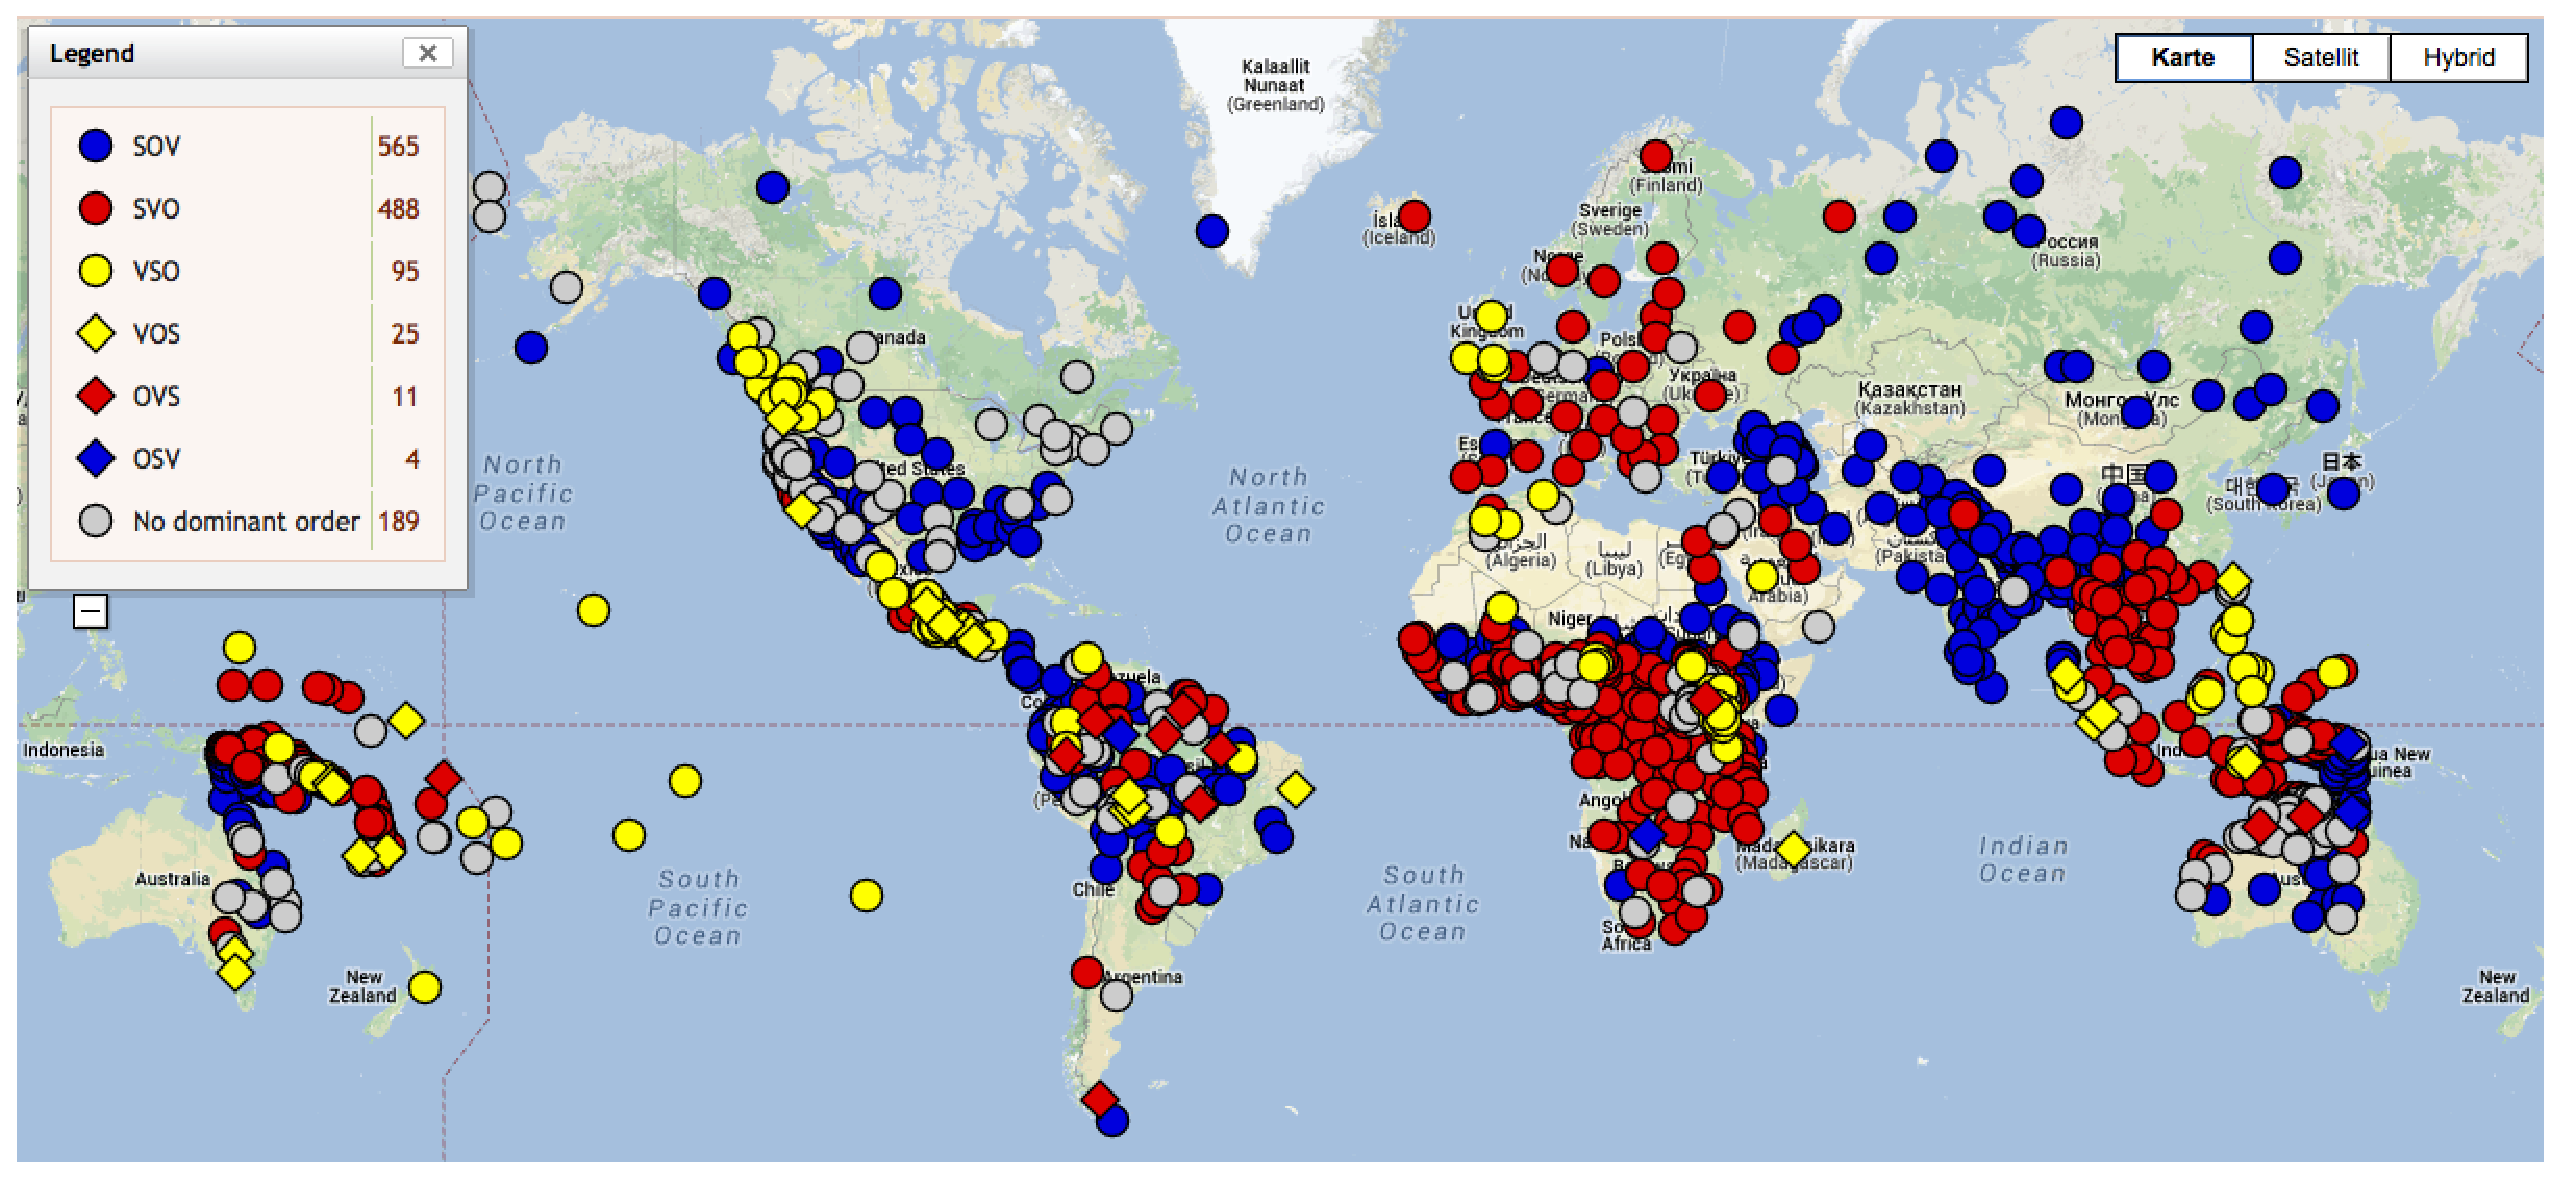
\includegraphics[width=\textwidth]{Bilder/WALS-SOV}

\vfill

{\small Matthew S. Dryer: Feature 81A: Order of Subject, Object and Verb,\\
 The World Atlas of Language Structures} 


}

\frame{
\frametitle{Subjekt, Objekt und Verb im WALS}

\begin{itemize}
\item Subjekte sind die Argumente mit den eher agensartigen Eigenschaften.
\pause
\item Objekte sind die Argumente mit den eher patiensartigen Eigenschaften.
\pause
\item Das ist nicht unbedingt deckungsgleich mit einzelsprachlichen Definitionen von Subjekt.
\ea
Der Aufsatz interessiert mich.
\z
\item Dominante Abfolge (Dryer: Determining Dominant Word Order):

Where a language is shown on one of the word order maps as having a particular order as the dominant
order in the language, this means that it is either \blaubf{the only order possible} or the order
that is \blaubf{more frequently used}.


I base my classification of Macushi here on the frequency counts, and since no order is more than
twice as frequent as the next most frequent order, I treat this language as lacking a dominant order
of subject, object, and verb.


Deutsch, Niederländisch und Friesisch sind V2-Sprachen, \dash die SVO- und SVAuxOV-Stellungen kommen
durch die Voranstellung des Verbs zustande, die eine Funktion hat. Wir zählen diese Sprachen also
mit zu den SOV-Sprachen.

\end{itemize}



}

\frame{
\frametitle{Subjekt, Objekt, Verb in Europa}

\begin{columns}[T]
\begin{column}{90mm}
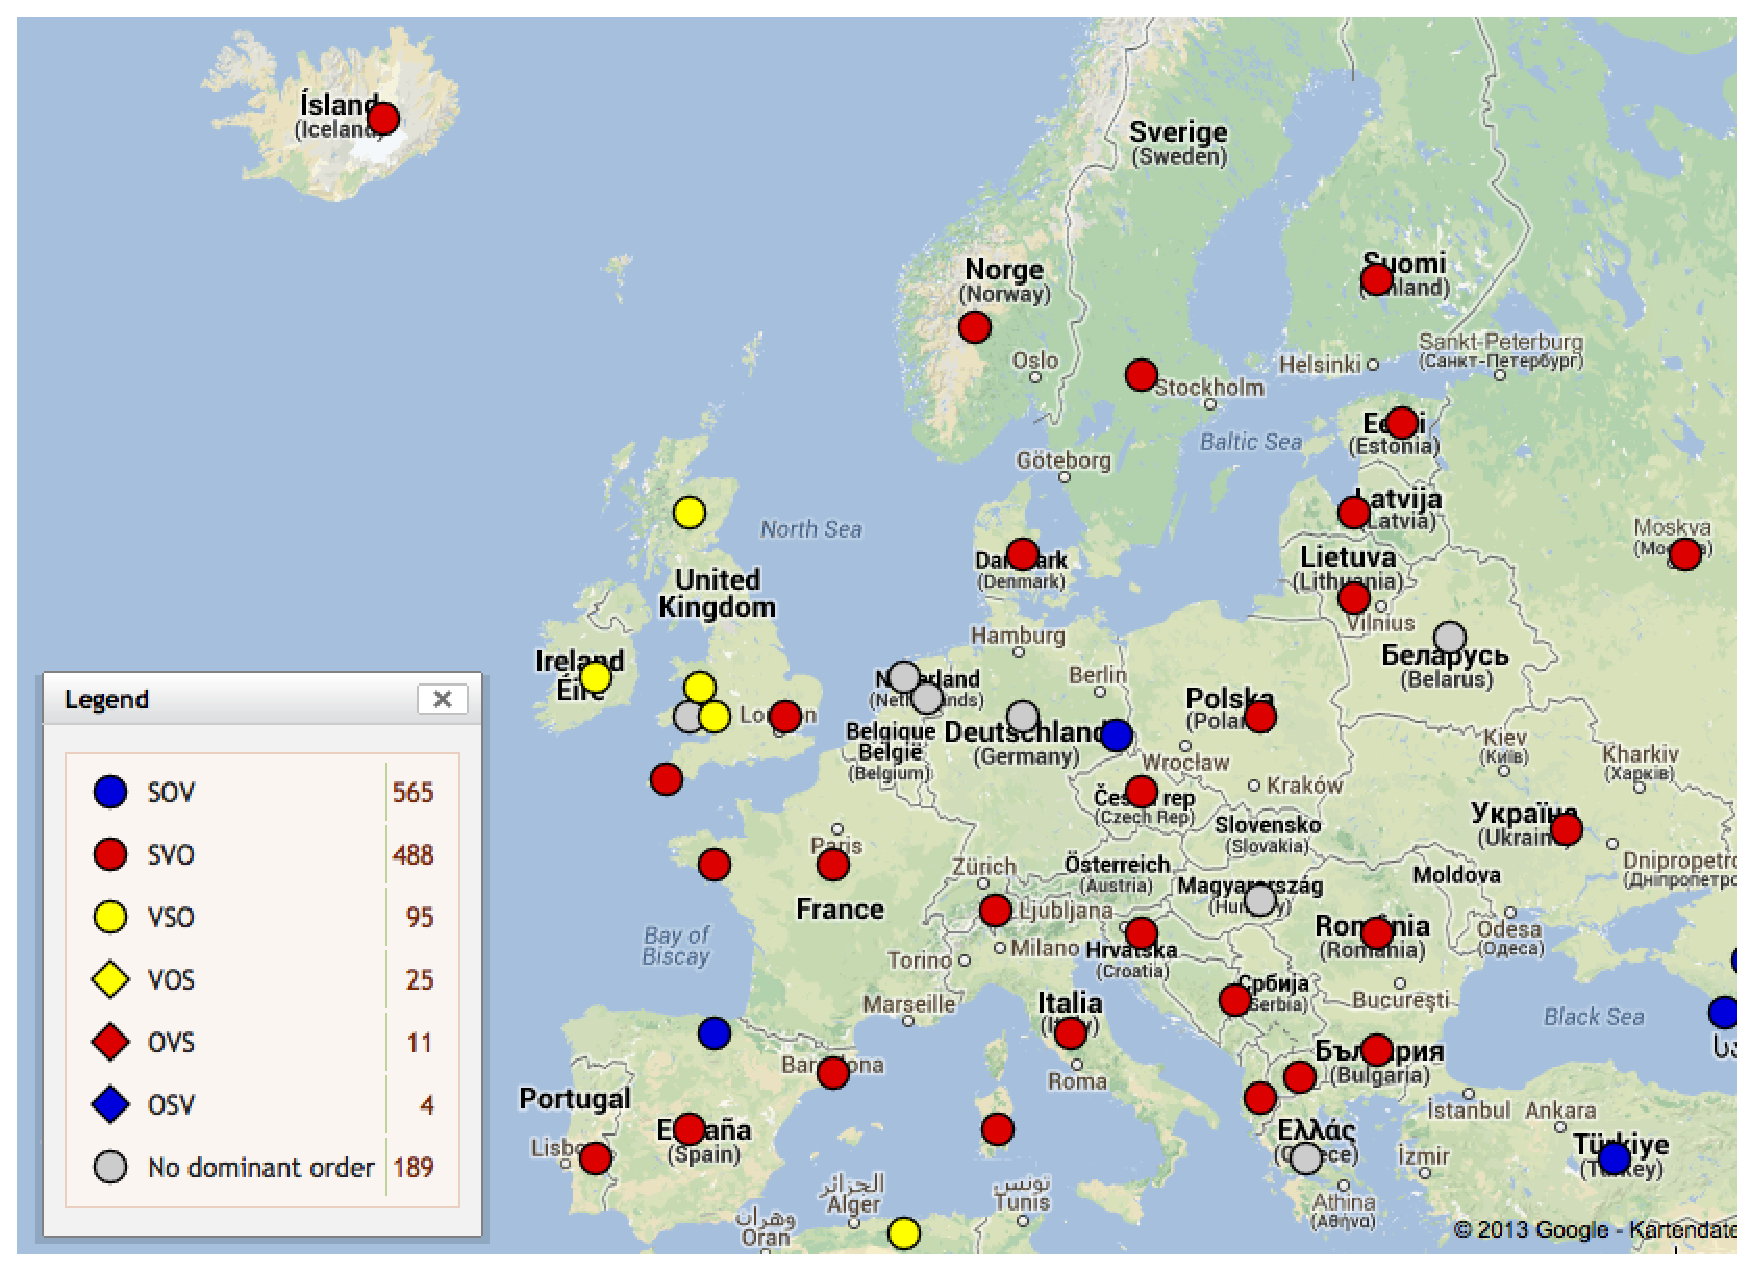
\includegraphics[width=\textwidth]{Bilder/WALS-SOV-Europa}
\end{column}
\begin{column}{25mm}
SVO:\\
Isländisch,\\
Norwegisch,\\
Schwedisch,\\
Dänisch,\\
Englisch
\end{column}
\end{columns}
}


\frame{
\frametitlefit{Dryer: Feature 81b: Two Dominant Orders of Subject, Object, and Verb}

\begin{columns}[T]
\begin{column}{90mm}
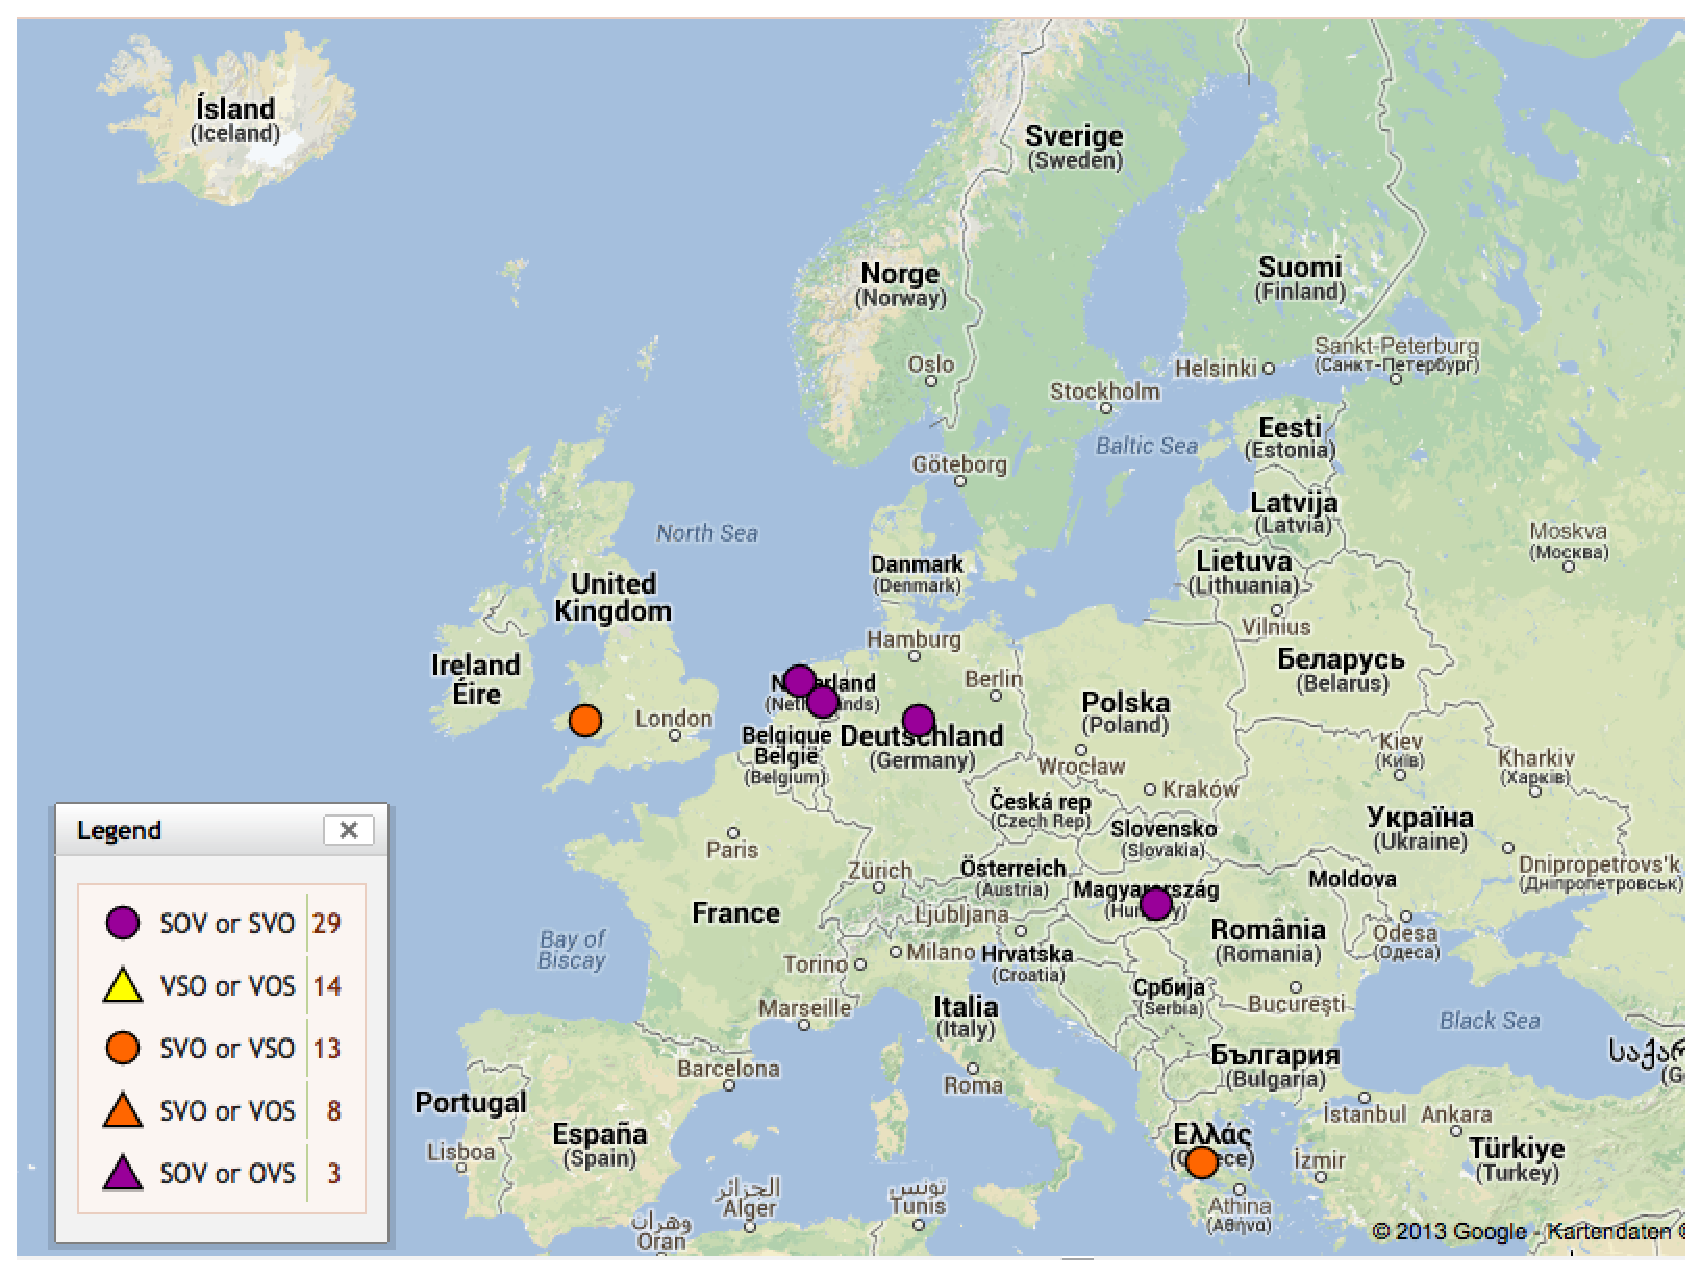
\includegraphics[width=.95\textwidth]{Bilder/WALS-SOV-Europa-no-dominant}
\end{column}
\begin{column}{30mm}
SVO oder SOV:\\
Deutsch,\\
Friesisch,\\
Niederländisch
\end{column}
\end{columns}
% Walisisch: SVO oder VOS
% Friesisch
% Niederländisch
% Deutsch 
% Ungarisch

}
% Eisenberg89:409 zitiert Greenberg66 mit Deutsch als SVO.


\frame{
\frametitle{Sprachen ohne dominante Konstituentenstellung im WALS}

Dryer:

A third subtype of language lacking a dominant order consists of languages in which different word
orders occur but the choice is syntactically determined. For example, in \blaubf{German and Dutch}, the
dominant order is \blaubf{SVO in main clauses lacking an auxiliary} and \blaubf{SOV in subordinate clauses and
clauses containing an auxiliary} [\ldots]. Because this results in both orders being
common, neither order is considered dominant here and these two languages are shown on the map as
lacking a dominant word order. In general, if the word order varies according to whether there is an
auxiliary verb, the language is shown on the map as lacking a dominant order.


}

\frame{
\frametitle{Hilfsverben zählen nicht, or do they?}

\eal
\ex Kim sieht den Fuchs.
\ex Kim hat den Fuchs gesehen.
\zl
Für Dreyer ist (\mex{0}a) SVO und (\mex{0}b) SAuxOV.\\
Aux wird ignoriert, so dass das Muster als SOV zählt.
\pause

Aber was ist mit (\mex{1})?
\eal
\ex Kim scheint den Fuchs zu sehen. \hfill(SVOV?)
\pause

\ex Kim scheint den Fuchs gesehen zu haben.
\zl

Es ist einfach das finite Verb, das aus Gründen der Satztypmarkierung anders plaziert wird.


}

\frame[shrink=5]{
\frametitle{OV vs.\ VO}

OV: Verben stehen nach dem Objekt:

\eal
\ex dass sie ihn sieht$_1$   \jambox{(Deutsch, SOV)}
\ex dass sie ihn gesehen$_2$ hat$_1$
\ex dass sie ihn gesehen$_3$ haben$_2$ muss$_1$
\zl

Einbettende Verben werden nach eingebetteten angeordnet.

\pause

VO: Verben stehen vor dem Objekt:

\eal
\ex
\gll at   hun ser$_1$ ham\\
     dass sie  sieht   ihn\\\jambox{(Dänisch, SVO)}
\ex
\gll at   hun have$_1$ set$_2$ ham\\
     dass sie  hat      gesehen ihn\\
\ex
\gll at hun må$_1$ have$_2$ set$_3$ ham\\
     dass sie muss haben gesehen ihn\\
\zl

OV: Deutsch, Niederländisch, Afrikaans, \ldots

VO: Englisch, Dänisch, Norwegisch, Schwedisch, \ldots

}

\frame{
\frametitle{Partikelverben und Resultativkonstruktionen}

%[Section~15.2]
\citet{Haider2020a}: Weitere Unterschiede zwischen VO- und OV-Sprachen:

Partikelverben:
\eal
\ex Kim will \alert{look up} the information.      \hfill(Verb < Partikel)
\ex Kim wird die Information \alert{nachschlagen}. \hfill(Partikel < Verb)
\zl
\pause

Resultativkonstruktionen:
\eal
\ex Kim will \alert{fish} the pond \alert{empty}.       \hfill(Verb < Pred)
\ex Kim wird den Teich \alert{leer} \alert{fischen}.    \hfill(Pred < Verb)
\zl



}

\subsection{V2}

\frame{
\frametitle{V2}

\begin{itemize}
\item Das Deutsche ist eine V2-Sprache:\\
      Das finite Verb steht in Aussagesätzen und \emph{w}"=Fragen an zweiter Stelle.
\item Davor kann eine beliebige Konsitutente stehen:
\eal
\ex Das Kind  gibt dem Eichhörnchen jetzt eine Nuss.
\ex Dem Eichhörnchen gibt das Kind jetzt eine Nuss.
\ex Eine Nuss gibt das Kind dem Eichhörnchen jetzt.
\ex Jetzt gibt das Kind dem Eichhörnchen eine Nuss.
\zl
\eal
\ex Wer gibt dem Eichhörnchen jetzt eine Nuss?
\ex Wem gibt das Kind jetzt eine Nuss?
\ex Was gibt das Kind dem Eichhörnchen jetzt?
\ex Wann gibt das Kind dem Eichhörnchen eine Nuss?
\zl
\end{itemize}

}

\frame{
\frametitle{V2 vs.\ Nicht-V2}

\begin{itemize}
\item Bis auf das Englische sind die germanischen Sprachen V2-Sprachen:
\eal
\ex Bagels mag ich.\jambox{(Deutsch)}
\ex Bagels, I like.\jambox{(Englisch)}
\zl 


\eal
\ex Gestern gab ich dem Eichhörnchen eine Nuss.\jambox{(Deutsch)}
\ex Yesterday, I gave the squirrel a nut.\jambox{(Englisch)}
\zl 

\item Es gibt Voranstellung im Englischen, diese erfolgt aber immer vor das Subjekt und das Verb.

\end{itemize}

}

\frame{
\frametitle{Nicht extrahierbare Elemente}

In den V2-Sprachen können fast alle Argumente vorangestellt werden. 

Im Englischen (sprecherabhängig) nicht alle Objekte voranstellbar \citep[\page 258]{Hudson92a-u}:

\eal
\judgewidth{\%}
\ex[]{
We give children sweets.
}
\ex[]{
These sweets, we give children \_.
}
\ex[\%]{
These children, we give \_ sweets.
}
\zl

}

\frame{
\frametitle{Voranstellung über Satzgrenzen hinweg}



\ea
{}[Über dieses Thema]$_i$ habe ich sie gebeten, [[einen Vortrag \_$_i$~] zu halten]?\footnote{
Nach \citew[\page 21]{HN89b}.
}
\z

Analyse von V2 kann also nicht einfach Umstellung von Satzgenossen sein.


}


\frame{
\frametitle{V2 und OV/VO}

\begin{itemize}
\item V2 ist unabhängig von VO/OV. Dänisch ist SVO und V2.
\eal
\ex 
\gll Gert har læst bogen.\\
     Gert hat gelesen Buch.{\sc def}\\\jambox{(Dänisch)}
\ex
\gll Bogen har Gert læst.\\
     Buch.{\sc def} hat Gert gelesen\\\jambox{(Dänisch)}
\zl


\end{itemize}

}

\frame{
\frametitle{Englisch als Residual V2}

Im Englischen gibt es Reste von V2-Strukturen in Fragen:
\eal
\ex Which book did Sandy read?
\ex Which book did Sandy give to Kim?
\ex To whom did Sandy give the book?
\zl

\citet[\page 375]{Rizzi1990a-u}:  \emph{residual V2 language}



}


\frame{
\frametitle{Satztypen}

Satztypen werden über Verbstellung kodiert. Neben Aussagesätzen und \emph{w}-Fragesätzen gibt es
auch V2-Imperative:

\ea
Jetzt gib ihr das Buch!
\z
\pause

Ansonsten: Entscheidungsfragen und Imperative als V1:
\eal
\ex Gibt er ihr das Buch?
\ex Gib ihr das Buch!
\zl

} 


\frame{
\frametitle{V2 ist selten}

V2 ist selten \citep[\page 343]{Holmberg2015a}.

\begin{itemize}
\item germanische Sprachen (außer Englisch, \citealp{HP86a-ed})
\item modernes Bretonisch \citep{BK2000a-u}
\item Estnisch
\item Altfranzösisch \parencites[Section~1.3]{Adams1987a-u}[Section~2.1.2]{Roberts93a-u}[Chapter~2]{Vance97a-u},
  Altitalienisch, Altspanisch \citep[Section~3.3.2]{Fontana97a-u}, 
\item Rätoromanisch \citep{Poletto2002a-u,Anderson2006a-u},
\item das Kashmiri (Indien, Pakistan, \citealp[Chapter~4]{Bhatt99a-u})
\item Inguschisch (autonomen Republik Inguschetien, Russische Föderation)
\item die austronesischen Sprachen Taiof und Sisiqa, \citep[\page 495]{Ross2004a-u} % wieder aus der englischen Wikipedia verschwunden
\item die Sprache brasilianischer Ureinwohner*innen Karitiana aus der Tupí-Familie \citep{Storto2003a-u} 
% Ist vielleicht nur X2 sowas wie die australischen Sprachen (Bayer2010)
%\item die uto-aztekische Sprache Tohono O'odham\\
%      (Südwesten der USA sowie im Norden Mexikos).
\end{itemize}



}





\subsection{Scrambling}

\frame{
\frametitle{Scrambling oder nicht}

Germanische OV-Sprachen (Deutsch, \ldots):\\
prinzipiell alle Abfolgen von Argumenten möglich:
\eal
\ex {}[weil] \rot{das Kind} \gruen{dem Eichhörnchen} \blau{die Nuss} gibt
\ex {}[weil] \rot{das Kind} \blau{die Nuss} \gruen{dem Eichhörnchen} gibt
\ex {}[weil] \blau{die Nuss} \rot{das Kind} \gruen{dem Eichhörnchen} gibt
\ex {}[weil] \blau{die Nuss} \gruen{dem Eichhörnchen} \rot{das Kind} gibt
\ex {}[weil] \gruen{dem Eichhörnchen} \rot{das Kind} \blau{die Nuss} gibt
\ex {}[weil] \gruen{dem Eichhörnchen} \blau{die Nuss} \rot{das Kind} gibt
\zl

\pause

Germanische VO-Sprachen (Englisch, \ldots): Argumente haben eine feste Stellung.
\eal
\ex because \rot{the child} gives \gruen{the squirrel} \blau{the nut}
\ex because \rot{the child} gives \blau{the nut} \gruen{to the squirrel} 
\zl
\emph{Dative Shift} erfordert Umkategorisierung. Markierung durch Präposition.


}

\subsection{Stellung der Adverbialien}

\frame{
\frametitle{Stellung der Adverbialien}


Deutsch, Niederländisch, \ldots: Stellung der Adverbien frei:
\eal
\ex weil das Kind dem Eichhörnchen die Nuss \blauit{gestern} gab
\ex weil das Kind dem Eichhörnchen \blauit{gestern} die Nuss gab
\ex weil das Kind \blauit{gestern} dem Eichhörnchen die Nuss gab
\ex weil \blauit{gestern} das Kind dem Eichhörnchen die Nuss gab
\zl

\pause

Dänisch, Englisch, \ldots: Adverbien stehen vor oder nach der VP:
\eal
\ex because the child \blauit{often} [\gruen{gave the squirrel the nut}]
\ex because the child [\gruen{gave the squirrel the nut}] \blauit{often}
\zl

\pause
Extremfall verschachtelte VPen \citep[§ 8.20, 495]{QGLS85a-u}:
\ea
It [\blauit{certainly} [\sub{VP} may [\blauit{possibly} [\sub{VP} have [\blauit{indeed} [\sub{VP} been\\ {}[\blauit{badly} [\sub{VP} formulated]]]]]]]].
\z

}


\subsection{Eingebettete Sätze}

\subsubsection{Konjunktional eingeleitete Nebensätze}

\frame{
\frametitle{Deutsch: eingebettete Sätze sind VL}

\begin{itemize}
\item Deutsch, Niederländisch, \ldots: V-letzt:

\ea
Ich weiß, dass Aicke das Buch heute gelesen hat.
\z

\pause
Stellung der anderen Konstituenten ist frei:
\eal
\ex Ich weiß, dass das Buch Aicke heute gelesen hat.
\ex Ich weiß, dass das Buch heute Aicke gelesen hat.
\zl

\end{itemize}

}

\frame{
\frametitle{Englisch: eingebettete Sätze SVO}


\begin{itemize}
\item Englisch: eingebettete Sätze SVO
\ea[]{
I  know that Kim has read the book yesterday.
}
\z

%% \pause
%% Andere Stellungen sind nicht möglich:
%% \eal
%% \ex[*]{
%% I know that has Max read the book yesterday.
%% }
%% \ex[*]{
%% I know that yesterday Max has read the book.
%% }
%% \zl

\end{itemize}

}



\frame{
\frametitle{Dänisch: eingebettete Sätze SVO oder V2}


\begin{itemize}
\item Dänisch: eingebettete Sätze SVO oder V2
\ea[]{
\gll Jeg  ved, at   Gert ikke  har læst  bogen          {i dag}.\\
     ich weiß dass Gert nicht hat gelesen Buch.{\sc def} heute\\\jambox{(SVO)}
}
\z
Negation hilft, Verbstellung zu bestimmen:
\ea[]{
\gll Jeg  ved, at   Gert har ikke  læst  bogen          {i dag}.\\
     ich weiß dass Gert hat nicht gelesen Buch.{\sc def} heute\\\jambox{(V2)}
}
\z



\pause
Andere Konstituenten in Initial-Stellungen sind möglich, \dash klares V2:
\eal
\ex[]{
\gll Jeg  ved, at   {i dag} har Gert ikke læst bogen.\\
     ich weiß dass heute   hat Gert nicht gelesen Buch.{\sc def}\\
}
\ex[]{
\gll Jeg ved, at   bogen          har Gert ikke  læst {i dag}.\\
     ich weiß dass Buch.{\sc def} hat Gert nicht gelesen heute\\
}
\zl

%% \ex[*]{
%% \gll Jeg  ved, at   {i dag} Gert har læst bogen.\\
%%      ich weiß dass heute   Gert hat gelesen Buch.{\sc def}\\
%% }
%%
%% \ex[*]{
%% \gll Jeg  ved, at   bogen          Gert har læst {i dag}.\\
%%      ich weiß dass Buch.{\sc def} Gert hat gelesen heute\\
%% }
%% \zl

\end{itemize}

}


\frame{
\frametitle{Jiddisch, Isländisch: eingebettete Sätze sind V2}

% Isländisch: Wikipedia (en)

\begin{itemize}
\item Jiddish: eingebettete Sätze sind V2 \citep[]{Diesing90a}:
\eal
\ex
\gll Ikh meyn  az   haynt hot Max geleyent dos bukh.\footnotemark\\
     ich   denke dass heute hat Max gelesen   das Buch\\
\footnotetext{\citew[\page 58]{Diesing90a}.}
\glt `Ich denke, dass Max heute das Buch gelesen hat.'

\ex% check!
\gll Ikh meyn  az   dos bukh hot Max geleyent.\\
     ich denke dass das Buch hat Max gelesen\\

\zl

\pause
Isländisch:
\ea 
\gll Engum         datt í hug,  að   vert  væri að reyna til     að kynnast honum.\footnotemark\\
     no.one.\DAT{} fell to mind that worth was  to try   \PREP{} to know    him\\\icelandic
\footnotetext{\citew[\page 75]{Maling90a-u}.}
\glt `It didn't occur to anyone that t was worth trying to get to know him.'
\z



\end{itemize}

}


\subsubsection{Interrogativnebensätze}


\frame{
\frametitle{Deutsch: Interrogativnebensätze \emph{w} + VL}

\begin{itemize}
\item Deutsch, Niederländisch, \ldots: \emph{w} + V-letzt:

\eal
\ex Ich weiß, wer heute das Buch gelesen hat.
\ex Ich weiß, was Aicke heute gelesen hat.
\zl

Interrogativnebensätze beginnen mit einer \emph{w}-Phrase.

\pause
\item Die \emph{w}-Phrase kann von weit her kommen:
\ea
Ich weiß nicht, [\gruen{über welches Thema}]$_i$ sie versprochen hat,\\
{}[[einen Vortrag \_$_i$] zu halten].
\z

\pause
\item Stellung der anderen Konstituenten ist frei:
\eal
\ex Ich weiß, was keiner diesem Eichhörnchen geben würde.
\ex Ich weiß, was diesem Eichhörnchen keiner geben würde.
\zl



\end{itemize}

}

\frame{

\frametitle{Dänisch, English: Interrogativnebensätze  \emph{w} + SVO}


\begin{itemize}
\item Dänisch: Interrogativnebensätze sind \emph{w} + SVO

\eal
\ex
\gll Jeg ved, hvad Gert har givet ham.\\
     ich weiß was Gert  hat gegeben ihm\\
\glt `Ich weiß, was Gert ihm gegeben hat.'
\ex
\gll Jeg ved, hvem Gert har givet   bogen.\\
     ich weiß wem  Gert hat gegeben Buch.{\sc def}\\
\glt `Ich weiß, wem Gert das Buch gegeben hat.'
\zl

\end{itemize}

}

\frame{
\frametitle{Jiddish: Interrogativnebensätze \emph{w} + V2}

\begin{itemize}
\item Jiddish: Interrogativnebensätze \emph{w} + V2 \citep[Abschnitte~4.1, 4.2]{Diesing90a}

%% \ea
%% %\ex
%% \label{vosmaks}
%% \gll Ikh veys nit   [vos Max hot gegesn].\footnotemark\\
%%      ich weiß nicht \hspaceThis{[}was Max hat gegessen\\
%% \footnotetext{\citew[S.\,68]{Diesing90a}.}
%% \glt `Ich weiß nicht, was Max gegessen hat.'

%% %% \ex%check
%% %% \gll Ikh veys nit   [vos              hot Max gegesn].\footnotemark\\
%% %%      ich weiß nicht \hspaceThis{[}was heute hat Max gegessen\\
%% %% \footnotetext{\citew[S.\,68]{Diesing90a}.}
%% %% \glt `Ich weiß nicht, was Max heute gegessen hat.'


\ea
\gll Ir veyst efsher [avu            do    voynt Roznblat   der goldshmid]?\footnotemark\\
     Sie wissen vielleicht  \spacebr{}wo da wohnt Roznblat der Goldschmied\\
\glt `Wissen Sie vielleicht, wo Roznblat der Goldschmied wohnt?' 
\footnotetext{
\citew[S.\,65]{Diesing90a}. Zitiert aus Olsvanger, \emph{Royte Pomerantsn}, 1949
}
\z
\end{itemize}

}



\subsection{Expletiva zur Satztypmarkierung}

\frame{
\frametitle{Expletiva zur Satztypmarkierung}

\begin{itemize}
\item Germanische Sprachen benutzen Expletiva, um Satztypen kenntlich zu machen,
      falls keine andere Konstituente die entsprechende Position füllt.
\pause
\item Deutsch V2-Hauptsätze

\eal
\ex Drei Reiter ritten zum Tor hinaus.
\ex \rot{Es} ritten drei Reiter zum Tor hinaus.
\zl
\end{itemize}


}

\frame{
\frametitle{Dänisch: \emph{w}-Sätze mit extrahiertem Subjekt}

\begin{itemize}
\item Dänisch: \emph{w} + SVO\\
      Bei Subjektextraktion muss Extraktion explizit kenntlich gemacht werden:
\eal
\ex[]{
\gll Politiet ved ikke, \gruen{hvem} \rot{der}   havde placeret bomben.\\
     Polizei.{\sc def} weiß nicht wer {\sc expl} hat plaziert Bombe.{\sc def}\\
\glt `Die Polizei weiß nicht, wer eigentlich die Bombe plaziert hat.'
}
\ex[*]{
\gll Politiet ved ikke, \gruen{hvem} havde placeret bomben.\\
     Polizei.{\sc def} weiß nicht wer hat plaziert Bombe.{\sc def}\\
}
\zl

\pause

Expletivum macht Extraktion sichtbar:
\eal
\ex[*]{ 
\gll [\gruen{hvem}$_i$     [\trace$_i$ havde placeret bomben]]\\
     \spacebr{}wer {}          hat   plaziert Bombe.\textsc{def}\\\danish
}
\ex[]{
\gll [\gruen{hvem}$_i$     [\rot{der}                    havde \trace$_i$ placeret bomben]]\\
     \spacebr{}who \spacebr{}\textsc{expl} hat   {}         plaziert Bombe.\textsc{def}\\
}
\zl


\end{itemize}

}

\frame{
\frametitle{Jiddish: \emph{w}-Sätze mit extrahiertem Subjekt}

\begin{itemize}
\item Jiddish: Interrogativnebensätze \emph{w} + V2\\
%% \ea
%% \label{vosmaks}
%% \gll Ikh veys nit   [vos Max hot gegesn].\footnotemark\\
%%      ich weiß nicht \hspaceThis{[}was Max hat gegessen\\
%% \footnotetext{\citew[S.\,68]{Diesing90a}.}
%% \glt `Ich weiß nicht, was Max gegessen hat.'
%% \z
%% \pause
%% \item 
  Wenn das Subjekt extrahiert wird, oder kein anderes Element ins Vorfeld soll, muss dort ein
  \emph{es} stehen:

\eal
\ex[]{
\gll ikh hob  zi  gefregt \gruen{ver} \rot{es}         iz beser  far ir\\
     I   have her asked   who {\sc expl} is better for her\\
\glt `I have asked her who is better for her.'}
\ex[]{
\gll ikh hob  im  gefregt \gruen{vemen} \rot{es}        kenen ale dayne khaverim\\
     I   have him asked   whom {\sc expl} know  all your friends\\
\glt `I asked him whom all your friends know.'}
\zl

\end{itemize}

}

\subsection{Verbalkomplexbildung}


\frame{
\frametitle{Verbalkomplexbildung nur in OV-Sprachen}

\begin{itemize}
\item Normalerweise stehen Objekte neben ihren Verben:
\ea
Somebody promised him [to read a book].
\z
\ea
weil    jemand   [ihr [das Buch zu lesen] versprochen] hat\\
\z

\pause

\item Deutsch, Niederländisch erlauben Verbalkomplexbildung:
\ea
weil \highlight{es}<2> \highlight{ihr}<3> \highlight{jemand}<4> \highlight{zu lesen}<2> \highlight{versprochen}<3> \highlight{hat}<4>. \citep{Haider90b}
\z

\pause
\pause
\pause
Die Verben am Ende verhalten sich wie ein einfaches Verb $\to$\\
Umordnung der Argumente ist möglich.


\pause
\item Englisch, Dänisch, \ldots{} erlauben keine Umordnung von Konstituenten

\eal
\judgewidth{\#}
\ex[*]{
Somebody promised a book her to read.
}
\ex[\#]{
Somebody promised to read her a book.
}
\zl

\end{itemize}


}

\subsection{Obligatorische Subjekte}

\frame{
\frametitle{Obligatorische Subjekte}

\begin{itemize}
\item Englisch, Dänisch brauchen ein Subjekt

\pause
\item Deutsch kommt ohne Subjekt klar:
\eal
\ex Ihm graut vor der Prüfung.
\ex Heute wird nicht gearbeitet.
\zl

\pause
\item Oft kann bei subjektlosen Verben ein expletives Subjekt angeschlossen werden:
\ea
Ihm graut es vor der Prüfung.
\z
\pause
\item Aber manchmal geht auch das nicht:
\eal
\ex[]{
Mir ist schlecht.
}
\ex[*]{
Mir ist es schlecht.
}
\ex[*]{
weil es mir schlecht ist
}
\zl
%% Das geht mit "etwas" oder "viel" aber das sind wohl adverbiale Akkusative, sie können nicht durch
%% Pronomina ersetzt werden.
%% \eal
%% \ex[]{
%% Mir liegt an dir.
%% }
%% \ex[*]{
%% Mir liegt es an dir.
%% }
%% \zl

\end{itemize}

}


\subsection{Kasus}

\frame{
\frametitle{Kasus}

\begin{itemize}
\item Isländisch hat das am besten erhaltene Flexionssystem.
\pause
\item Im Vergleich zu anderen germanischen Sprachen ist Isländisch interessant,\\
      weil es Subjekte hat, die nicht im Nominativ stehen \citep{ZMT85a}.
\pause
\item Einheitliche Behandlung der Kasuszuweisung ist möglich:\\
\citew*{YMJ87}.

\end{itemize}


}

\subsection{Unpersönliches Passiv}

\frame[shrink]{
\frametitle{Unpersönliches Passiv}

\begin{itemize}
\item Das Deutsche erlaubt ein unpersönliches Passiv:
\ea[]{
\label{ex-gearbeitet-wurde}
weil noch gearbeitet wird
}
\z

\pause
\item Das Englische lässt kein unpersönliches Passiv zu.
\ea[*]{
because (it) was worked
}
\z

\pause
\item Dänisch schon, trotz Subjektbedingung: Expletivum wird eingefügt.
\eal
\label{ex-bliver-arbejder}
\ex 
\gll fordi der bliver arbejdet\\
     weil {\sc expl} wird gearbeitet\\
\glt `weil gearbeitet wird'
\ex
\gll fordi   der arbejdes\\
     weil  {\sc expl} arbeiten.{\sc pass}\\
\glt `weil gearbeitet wird'
\zl
\pause
\item Das Deutsche erlaubt kein Expletivum.

\end{itemize}
\pause\pause\pause

}


% %% -*- coding:utf-8 -*-

\subtitle{Phrsaenstrukturgrammatiken und \xbar-Theorie}

\section{Phrsaenstrukturgrammatiken und \xbar-Theorie}


\huberlintitlepage[22pt]


% %% -*- coding:utf-8 -*-
\author{Stefan Müller}

\subtitle{Valenz, Argumentanordnung und Adjunktstellung}

\section{Valenz, Argumentanordnung und Adjunktstellung}


\huberlintitlepage[22pt]


\outline{

\begin{itemize}
\item {Überblick über die germanischen Sprachen}
\item Phänomene
\item Phrasenstrukturgrammatiken und \xbart
\item \alert{Valenz, Argumentanordnung und Adjunkte}
\item Verbalkomplexbildung in den SOV-Sprachen
\item Verbstellung: Verberst- und Verbzweitstellung
\item Passiv
\item Eingebettete Sätze
\end{itemize}

}



\frame{
\frametitle{Literaturhinweis}



Zu diesem Abschnitt lesen Sie bitte \citew[Kapitel~4]{MuellerGermanic}.

\begin{refsection}

\nocite{MuellerGermanic}

\printbibliography[heading=none,notkeyword=this]

\end{refsection}

\pause

Die Theorie, die wir behandeln werden, ist Head-Driven Phrase Structure Grammar in einer
abgerüsteten Version.

Zu HPSG siehe \citew{ps,ps2,Sag97a,MuellerLehrbuch,HPSGHandbook}.



}

\subsection{Valenz}



\frame{
\frametitle{Vorhandensein bestimmter Konstituenten}

Die Wortfolgen in (\mex{1}) sind keine wohlgeformten Sätze:
\eal
\ex[*]{
\dass der        Delphin erwartet
}
\ex[*]{
\dass des        Kindes       der       Delphin den        Ball dem        Kind  gibt
}
\zl
Bei (\mex{0}a) fehlt etwas, bei (\mex{0}b) ist etwas zu viel.


}

\frame{
\frametitle{Valenz in der Chemie und in der Linguistik}


\citet{Tesniere59a-de} übernimmt das Konzept der Valenz aus der Chemie:


\vfill

\centerline{
\begin{forest}
[O
  [H] 
  [H] ]
\end{forest}
\hspace{5em}
\begin{forest}
[kennen
 [Aicke]
 [Conny] ]
\end{forest}
}

\vfill

}

\frame{
\frametitle{Argumente}

NPen in (\mex{1}) sind Argumente der jeweiligen Verben:
\eal
\ex[]{
%\gll
\dass der        Delphin den        Menschen erwartet\\
%     \that{}  the.\NOM{} dolphin den.\ACC{} human   expects\\
%\glt `that the dolphin expects the human'
}
\ex[]{
%\gll 
{}[dass] der        Delphin dem        Kind  den        Ball gibt\\
%     \that{}  the.\NOM{} dolphin the.\DAT{} child the.\ACC{} ball gives\\
%\glt `that the dolphin gives the child the ball'
}
\zl

Meistens füllen syntaktische Argumente auch eine semantische Rolle (\zb Gebender, Agens, Actor,
\ldots).\nocite{Dowty91a,VanValin99a-u}

\citet[Chapter~48]{Tesniere2015a-u}: 

Theaterszene: Was wird minimal gebraucht, um einen Geben-Vorgang zu spielen?

\begin{itemize}
\item einen Geber*in
\item etwas Gegebenes
\item einen Empfänger*in
\end{itemize}

}

\frame{
\frametitle{Adjunkte}

\begin{itemize}
\item Zusätzlich zu den Argumenten können Adjunkte im Satz vorkommen:

\eal
\ex
%\gll
\dass{} der        Delphin dem        Kind  \alert{schnell} den        Ball gibt\\
% \that{} the.\NOM{} dolphin the.\DAT{} child quickly the.\ACC{} ball gives\\
%\glt `that the dolphin gives the child the ball quickly'
\ex that the dolphin gives the child the ball \alert{quickly}
\zl

\pause

\item Adjunkte tragen zusätzliche Information bei, füllen aber keine semantische Rolle.

\end{itemize}

}

\frame{
\frametitle{Optionale Argumente}

Argumente können fast immer weggelassen werden, wenn der Kontext entsprechende Information enthält.

\eal
\ex 
%\gll 
Sie gibt Geld.
%     she gives money\\
%\glt `She gives money.'
\ex 
%\gll 
Sie gibt den Armen.
%     she gives the poor\\
%\glt `She gives to the poor.'
\ex\label{ex-sie-gibt} 
%\gll 
Sie gibt.
%     she gives\\
\ex 
%\gll 
Gib!
%     give\\
\zl

Im Kontext eines Skat-Spiels ist klar, was gegeben wird und wer die Empfänger sind.

Bei einigen wenigen Verben kann man die Argumente nicht weglassen:
\eal
\ex verschlingen
\ex erwarten
\zl

Argumente können optional sein, Adjunkte sind es immer.


}

\frame{
\frametitle{Chemie und optionale Elemente}

Die Analogie zu chemischen Verbindungen ist hilfreich, aber die optionalen Argumente sind verwirrend:
\eal
\ex Kirby helps Sandy.
\ex Kirby helps.
\zl

\hfill
\begin{forest}
[O
  [H] 
  [H] ]
\end{forest}
\hspace{5em}
\begin{forest}
[helps
 [Kirby]
 [Sandy] ]
\end{forest}
\hfill\mbox{}

Lösung: Unterscheidung zwischen syntaktischer und semantischer Valenz.

Die Theateranalogie hilft uns, semantische Argumente zu finden,\\
die Analogie zur Chemie taugt eher für syntaktische Argumente. 

Man muss ein spezielles, syntaktisch einstelliges Verb für (\mex{0}b) annehmen.

}

\frame{
\frametitle{Shoppen statt Drama}

\begin{itemize}
\item Vergleich mit Einkauf besser:\\
Wir wollen Nudeln mit Tofu und Tomatensoße machen.

Für Tomatensoße brauchen wir Zwiebeln.

\item Alle Zutaten kommen auf die Einkaufsliste.

\item Im Laden merken wir, dass es keinen Tofu gibt.

\item Macht nichts, geht auch ohne: Tofu ist optional.

\item Nudeln gibt es. 10.000 Sorten.

\item Tomaten und Zwiebeln. Fertig.

\item Ach. Gummibärchen. Wie? Standen nicht auf der Liste?

Gummibären sind Adjunkte!

\end{itemize}

}

\frame{
\frametitle{Nudeln, Tomaten, Zwiebeln und Syntax}

\begin{itemize}
\item Es gibt mehrere Wege, sicherzustellen, dass alles, was gebraucht wird, da ist.

\item Phrasenstrukturen wie bei GPSG (siehe vorige Sitzung)

\ea
\label{ditrans-schema-two}
\begin{tabular}[t]{@{}l@{ }l@{ }l}
S  & $\to$ & NP[\type{nom}] NP[\type{dat}] NP[\type{acc}] V[\type{ditransitive}]\\
\end{tabular}
\z

\pause
\item Diese wurden dann aber für lexikon-orientierte Ansätze aufgegeben.\\
  \parencites{Jacobson87b}[Section~5.5]{MuellerGT-Eng1}{MWArgSt}
\pause
\item Gründe: 
\begin{itemize}
\item Voranstellung von Teilphrasen (Partial VP Fronting)\\ \citep{Nerbonne86a,Johnson86a} 
\pause
\item Interaktionen mit Morphologie \citep[Section~5.5.1]{MuellerGT-Eng1}
\end{itemize}
\pause
\item Come Back der phrasalen Ansätze in Construction Grammar \citep{Goldberg95a}, diese
  funktionieren aber nicht.

\parencites{Mueller2006d,MuellerPersian,MuellerUnifying,MWArgSt,MWArgStReply,MuellerFCG,MuellerLFGphrasal,MuellerPotentialStructure,MuellerGT-Eng4,MuellerCxG}

\end{itemize}

}

\frame{
\frametitle{Valenzlisten}

\begin{itemize}
\item Argumente werden in Listen repräsentiert:
\ea
\label{valence-specifications-German}
\begin{tabular}[t]{@{}l@{~}l@{~}l}
a. & \emph{schläft} `sleeps':        & \sliste{ NP[\type{nom}] }\\
b. & \emph{kennt} `knows':           & \sliste{ NP[\type{nom}], NP[\type{acc}] }\\
%b. & \emph{unterstützt} `supports':  & \sliste{ NP[\type{nom}], NP[\type{acc}] }\\
c. & \emph{hilft} `helps':           & \sliste{ NP[\type{nom}], NP[\type{dat}] }\\
d. & \emph{gibt} `gives':            & \sliste{ NP[\type{nom}], NP[\type{dat}], NP[\type{acc}] }\\
e. & \emph{wartet} `waits':          & \sliste{ NP[\type{nom}], PP[\type{auf}] }\\
\end{tabular}
\z

NP[\type{nom}] ist dann so was wie \emph{Nudeln}.\\
Es gibt ganz viele verschiedene Möglichkeiten, diese Valenzanforderung zu befriedigen: \emph{sie},
\emph{das Kind}, \emph{der lachende Delphin}, \ldots

\pause
\item Elemente der Listen sind in einer bestimmten Reihenfolge angeordnet. Diese entsprechen der
  Reihenfolge im Englischen und der unmarkierten Reihenfolge im Deutschen \citep{Hoehle82a}. 


\end{itemize}



}


\frame{
\frametitle{Valenzgesteuerter Strukturaufbau}

\vfill
\centerfit{
\begin{forest}
sm edges
[{S \eliste},visible on=6-
  [{NP[\type{nom}]},visible on=5- 
    [niemand,visible on=5-] ]
  [{V$'$\sliste{ \blau<4>{NP[\type{nom}]} } },visible on=3-
    [\blau<3>{NP[\type{acc}]}, visible on=2-
      [ihn,visible on=2-] ]
    [{V \sliste{ \blau<4>{NP[\type{nom}]}, \blau<3>{NP[\type{acc}]}}} [kennt]] ] ]
\end{forest}}

\vfill
\begin{itemize}
\item Valenzanforderung ist in einer Liste repräsentiert
\pause
\item Ein Element der Liste wird mit dem Kopf kombiniert.\\
\pause\pause
      Liste mit restlichen Elementen wird nach oben gegeben.
\pause\pause\pause
\item Wie einkaufen mit App:\\
      Ein Element nach dem anderen wird aus der Liste entfernt.
%\pause
%\item Wichtig: Die Theorie sagt nichts darüber aus welcher
\end{itemize}

}

\frame{
\frametitle{Beschränkungsbasierte Theorien und Psycholinguistik}

\centerfit{
\begin{forest}
sm edges
[{S \eliste},visible on=4-
%  [{[dass]},no edge,visible on=3-]
  [{NP[\type{nom}]},visible on=3- 
    [niemand,visible on=3-] ]
  [{V$'$\sliste{ NP[\type{nom}] } },visible on=4-
    [{NP[\type{acc}]},visible on=5- 
      [ihn,visible on=5-] ]
    [{V \sliste{ NP[\type{nom}], NP[\type{acc}] }},visible on=6- [kennt,visible on=7-]] ] ]
\end{forest}}

\begin{itemize}
\item Erklärungen im Folgenden immer von unten nach oben.
\pause
\item Das ist in Theorien wie HPSG aber nicht zwingend. 

Sehr wichtig aus psycholinguistischer Sicht, denn Verarbeitung ist inkrementell.
\parencites{Marslen-Wilson75a,TSKES96a,SW2011a,Wasow2021a}
\pause

\end{itemize}




}


\frame{
\frametitle{Optionale Argumente?}

\begin{itemize}
\item Es gibt mehrere Möglichkeiten, mit optionalen Argumenten umzugehen.
\item Die offensichtlichste: Wir haben alternative Lexikoneinträge.
% \ea
% \begin{tabular}[t]{@{}l@{~}l@{~}l}
% a. & \emph{gibt} `gives':            & \sliste{ NP[\type{nom}] }\\
% b. & \emph{wartet} `waits':          & \sliste{ NP[\type{nom}] }\\
% \end{tabular}
% \z
\ea
\begin{tabular}[t]{@{}l@{~}l@{~}l}
a. & \emph{gibt}:            & \sliste{ NP[\type{nom}] }\\
b. & \emph{wartet}:          & \sliste{ NP[\type{nom}] }\\
\end{tabular}
\z
\end{itemize}



}


\subsection{Scrambling}

\frame{
\frametitle{Scrambling: Konstituentenstellung im Deutschen}

\vfill
\centerfit{
\begin{forest}
sm edges
[{S \eliste}
   [{NP[\type{acc}]} [ihn] ]
   [{V$'$\sliste{ NP[\type{acc}] } }
      [{NP[\type{nom}]} [niemand] ]
      [{V \sliste{ NP[\type{nom}], NP[\type{acc}]}} [kennt] ] ] ]
\end{forest}}
\vfill
\pause
\begin{itemize}
\item Ein beliebiges Element der Liste kann mit Kopf kombiniert werden.\\
      $\to$ auch Abfolge Acc $<$ Nom analysierbar.\\
      Liste mit restlichen Elementen wird nach oben gegeben.
\end{itemize}

}



\subsection{SVO: Dänisch/Englisch}


\frame{
\frametitle{VP in SVO-Sprachen}

\begin{itemize}
\item Verben und Objekte bilden eine Wortgruppe:
\eal
\ex John promised to read the book and [\alert{read the book}], he will.
\ex He will [\alert{read the book}].
\ex Kim [[\alert{sold the car}] and [\alert{bought a bicycle}]]. 
\ex He often [\alert{reads the book}].
%\ex He [reads the book] often.
\ex \ldots{} [often [\alert{read the book}] slowly], he will.
\zl
\pause
\item Gut zu erfassen mit zwei Valenzlisten:\\
      eine für Komplemente (\comps für \textsc{complements}) und eine für das Subjekt (\textsc{spr} für \textsc{specifier}).
\end{itemize}


}

\frame{
\frametitle{Dänisch, Englisch, \ldots}

~\vfill

\centerfit{\begin{forest}
sm edges
[{V[\spr \eliste, \comps \eliste]}, name=S
   [{NP[\type{nom}]} [nobody] ]
   [V\feattab{
      \spr \sliste{ NP[\type{nom}] }, \comps \sliste{} }, name=VP
     [V\feattab{
         \spr \sliste{ NP[\type{nom}] },\\
         \comps \sliste{ NP[\type{acc}]}} [knows] ]
        [{NP[\type{acc}]} [him] ] ] ]
\node [right=4cm] at (S)
    {
        = S
    };
\node [right=4cm] at (VP)
    {
        = VP
    };
\end{forest}}


\vfill

\begin{itemize}
\item Englisch ist eine SVO-Sprache:\\
      Komplemente rechts des Verbs, Subjekt links
%\item Komplemente können nicht einfach umgestellt werden.
\item Komplemente bilden mit dem Verb zusammen eine Phrase (VP = \comps \sliste{}).

      Diese wird mit dem Subjekt kombiniert.
\end{itemize}

\vfill

}


\frame{
\frametitle{Kein Scrambling}

\begin{itemize}
\item Dänisch, Englisch:\\
      Elemente aus Valenzliste müssen von links nach rechts abgebunden werden.

\pause
\item Deutsch, Niederländisch:\\
      Elemente können in beliebiger Reihenfolge abgebunden werden.

%\pause
%\item 
\end{itemize}

}


\frame{
\frametitle{SVO: Ditransitive Verben: Abbindung von \comps von links}


\centerline{
\begin{forest}
sm edges
[{V[\spr \eliste, \comps \eliste]}, visible on=6-
   [{NP[\type{nom}]}, visible on=5- 
     [Kim, visible on=5-] ]
   [V\feattab{
      \spr \sliste{ NP[\type{nom}] }, \comps \sliste{}}, visible on=4-
     [V\feattab{
         \spr \sliste{ NP[\type{nom}] },\\
         \comps \sliste{ PP[\type{to}] }}, visible on=2-
       [V\feattab{
           \spr \sliste{ NP[\type{nom}] },\\
           \comps \sliste{ NP[\type{acc}], PP[\type{to}] }} [gave] ]
         [{NP[\type{acc}]} 
            [a book, roof] ] ]
       [{PP[\type{to}]}, visible on=3- 
         [to Sandy, roof, visible on=3-] ] ] ]
\end{forest}}

Bei kopffinalen Sprachen ohne Scrambling Abbindung von rechts.


}

%% \frame{
%% \frametitle{Regeln: Englisch und Deutsch}

%% \begin{itemize}
%% \item Englisch:
%% \ea
%% H[\comps \ibox{B}] $\to$ H[\comps \ibox{B} $\oplus$ \sliste{ \ibox{1} } ] ~~~\ibox{1}
%% \z

%% `$\oplus$' zerlegt Liste in zwei Teillisten.

%% \pause

%% \item Deutsch:
%% \ea
%% H[\comps \ibox{A} $\oplus$ \ibox{B}] $\to$ H[\comps \ibox{A} $\oplus$ \sliste{ \ibox{1} } $\oplus$ \ibox{B} ] ~~~\ibox{1}
%% \z

%% \pause

%% \item Das Englische unterscheidet sich vom Deutschen dadurch,\\
%%       dass \ibox{A} die leere Liste ist.

%% $\to$ Englisch ist restriktiver.

%% \end{itemize}


%% }


\frame{
\frametitle{Deutsch}



\centerfit{\begin{forest}
sm edges
[{V[\spr \eliste, \comps \eliste]}, name=S
        [{NP[\type{nom}]} [niemand] ]
        [{V\feattab{
              \spr \sliste{ }, \comps \sliste{ NP[\type{nom}] } }}, name = Vs
          [{NP[\type{acc}]} [ihn] ] 
          [V\feattab{
              \spr \sliste{  },\\
              \comps \sliste{ NP[\type{nom}], NP[\type{acc}]}} [kennt] ]
] ]
\node [right=4cm] at (S)
    {
        = S
    };
\node [right=4cm] at (Vs)
    {
        = V$'$
    };
\end{forest}}

Das Subjekt ist bei finiten Verben in der \compsl \citep{Pollard90a,Kiss95a}.

Abkürzungen: \begin{tabular}[t]{@{}l@{ = }l}
             S  & [\spr \eliste, \comps \eliste]\\
             VP & [\spr \sliste{ NP[\type{nom}] }, \comps \sliste{}]\\
             V$'$ & alle anderen V-Projektionen (außer Verbalkomplexen)\\
             \end{tabular}

}

\subsection{Immediate Dominance Schemata}

\frame{
\frametitle{Immediate Dominance Schemata}

\begin{itemize}
\item In vielen theoretischen Arbeiten werden einfach Baumstrukturen gezeigt.
\item Diese sind aber nicht einfach da.\\
      Es gibt Regeln oder Schemata, die sie lizenzieren.
\item \ZB \xbar-Schemata oder Regel für Phrasenstrukturen oder Dependenzstrukturen.
\item Regeln für HPSG:
\ea\label{schema-head-spr-and-head-comps-preliminary}
Specifier-Head Schema and Head-Complement Schema (preliminary)
\begin{tabular}[t]{@{}l@{ }l@{}}
H[\spr \ibox{1}]   & $\to$ H[\spr \ibox{1} $\oplus$ \sliste{ \ibox{2} }, \comps \eliste]\hspace{1em}\ibox{2}  \\
H[\comps \ibox{1}] & $\to$ H[\comps \sliste{ \ibox{2} } $\oplus$ \ibox{1}]\hspace{1em}\ibox{2} \\
\end{tabular}
\z
\pause
\item H steht für \emph{head}. Die entsprechende Phrase ist der oder enthält den Kopf.

\end{itemize}

}


\subsubsection{Spezifikator-Kopf-Strukturen}

\frame{
\frametitle{Schemata als Teilbäumchen}

\begin{itemize}
\item Schemata lassen sich auch als Teilbäumchen darstellen.
\ea\label{schema-head-spr-and-head-comps-preliminary}
Specifier-Head Schema (preliminary)\\
H[\spr \ibox{1}] $\to$ H[\spr \ibox{1} $\oplus$ \sliste{ \ibox{2} }, \comps \eliste]\hspace{1em}\ibox{2}
\z

\item Specifier-Head Schema in Baum-Notation:
\vfill
%\centerline{
\begin{forest}
[H\feattab{\spr \ibox{1}}%,\\
           %\comps \eliste}
  [\ibox{2}]
  [H\feattab{\spr \ibox{1} $\oplus$ \sliste{ \ibox{2} },\\
             \comps \eliste}
  ]]
\end{forest}
%}
\vfill

\end{itemize}

}

\frame{
\frametitle{\texttt{append} ($\oplus$)}

\begin{itemize}
\item \texttt{append} verknüpft zwei Listen: \sliste{ \normalfont a } $\oplus$ \sliste{ \normalfont b } =
\sliste{ \normalfont a, b }. 

\pause
\item Die Verknüpfung einer Liste L mit der leeren Liste ergibt die Liste L.

\pause
\item Beispiel: \texttt{append} teilt die Liste \sliste{ NP[\type{nom}], NP[\type{dat}], NP[\type{acc}
    ] } wie folgt:
\eal
\ex \oneline{\eliste{} $\oplus$ \sliste{ NP[\type{nom}], NP[\type{dat}], NP[\type{acc}] } = \sliste{ NP[\type{nom}], NP[\type{dat}], NP[\type{acc}] }}
\pause
\ex \oneline{\sliste{ NP[\type{nom}] } $\oplus$ \sliste{ NP[\type{dat}], NP[\type{acc}] } = \sliste{ NP[\type{nom}], NP[\type{dat}], NP[\type{acc}] }}
\pause
\ex \oneline{\sliste{ NP[\type{nom}], NP[\type{dat}] } $\oplus$ \sliste{ NP[\type{acc}] } = \sliste{ NP[\type{nom}], NP[\type{dat}], NP[\type{acc}] }}
\pause
\ex \oneline{\sliste{ NP[\type{nom}], NP[\type{dat}], NP[\type{acc}] } $\oplus$ \eliste{} = \sliste{ NP[\type{nom}], NP[\type{dat}], NP[\type{acc}] }}
\zl

\end{itemize}

}


\frame{
\frametitle{Zerlegung der Valenzliste}

\begin{itemize}
\item Specifier-Head Schema in Baum-Notation:\\
\vfill
\begin{forest}
[H\feattab{\spr \ibox{1}}%,\\
           %\comps \eliste}
  [\ibox{2}]
  [H\feattab{\spr \ibox{1} $\oplus$ \sliste{ \ibox{2} },\\
             \comps \eliste}
  ]]
\end{forest}
\vfill

\item Schema zerlegt Liste in beliebige Liste \iboxb{1} und eine einelementige Liste (\sliste{ \ibox{2} }).

\item Für unser Beispiel wäre das (\mex{0}c):
\ea
\oneline{\sliste{ NP[\type{nom}], NP[\type{dat}] } $\oplus$ \sliste{ NP[\type{acc}] } = \sliste{ NP[\type{nom}], NP[\type{dat}], NP[\type{acc}] }}
\z

\ibox{1} = \sliste{ NP[\type{nom}], NP[\type{dat}] } und \ibox{2} = NP[\type{acc}]

\end{itemize}

}

\frame{
\frametitle{Listenzerlegung in Spezifikator-Kopf-Strukturen}

\begin{itemize}
\item \sprl hat für gewöhnlich nur ein Element: NP[\type{nom}]/Subjekt für Verben in SVO-Sprachen oder
  Determiner, wenn der Kopf ein Nomen ist.

\vfill
\begin{forest}
[H\feattab{\spr \ibox{1}}%,\\
           %\comps \eliste}
  [\ibox{2}]
  [H\feattab{\spr \ibox{1} $\oplus$ \sliste{ \ibox{2} },\\
             \comps \eliste}
  ]]
\end{forest}

\vfill

\pause
\item \ibox{1} ist leere Liste, \ibox{2} ist NP[\type{nom}] bzw.\ Det. 


\eal
\ex \eliste{} $\oplus$ \sliste{ NP[\type{nom}] } = \sliste{ NP[\type{nom}] }
\ex \eliste{} $\oplus$ \sliste{ Det } = \sliste{ Det }
\zl

\end{itemize}

}

\exewidth{(235)}

\frame{
\frametitle{Kopf hat Wünsche. Schema regelt Passgenauigkeit}

\begin{itemize}
\item Beschreibung der Tochter muss mit der einzusetzenden Tochter kompatibel sein.

\vfill
\centerline{
\begin{forest}
[H\feattab{\spr \ibox{1}}%,\\
           %\comps \eliste}
  [\alert{\ibox{2}}]
  [H\feattab{\spr \ibox{1} $\oplus$ \sliste{ \alert{\ibox{2}} },\\
             \comps \eliste}
  ]]
\end{forest}}

\vfill
\ibox{2} wird vom Kopf bestimmt. Linke Tochter muss dazu passen.
\pause
\vfill
\hfill
\scalebox{.8}{%
\begin{forest}
sm edges
[V\feattab{\spr \eliste,\\
           \comps \eliste}
  [{\ibox{1} NP[\type{nom}]} [she]]
  [V\feattab{\spr \sliste{ \ibox{1} NP[\type{nom}] },\\
             \comps \eliste} [sleeps]]]
\end{forest}}
\hfill
\scalebox{.8}{%
\begin{forest}
sm edges
[V\feattab{\spr \eliste,\\
           \comps \eliste}
  [{\ibox{1} NP[\type{nom}]} [the brown squirrel,roof]]
  [V\feattab{\spr \sliste{ \ibox{1} NP[\type{nom}] },\\
             \comps \eliste} [sleeps]]]
\end{forest}}\hfill\mbox{}
\vfill

\end{itemize}

}

\frame{
\frametitle{Die \compsl im Spezifikatorschema}


\begin{itemize}
\item Die \compsl ist leer. 
\vfill
\centerline{
\begin{forest}
[H\feattab{\spr \ibox{1}}%,\\
           %\comps \eliste}
  [\ibox{2}]
  [H\feattab{\spr \ibox{1} $\oplus$ \sliste{ \ibox{2} },\\
             \comps \eliste}
  ]]
\end{forest}}
\vfill
Erst alle Komplemente mit einem Kopf kombiniert, dann der Spezifikator.
%\eal
%\ex {}[a [picture [of Kim]]]
\ea {}[The dolphin [attacked [the shark]]]
\z

\end{itemize}

}


\frame{
\frametitle{Nominalstrukturen}

\begin{itemize}
\item Neben NP + VP-Strukturen wird das Spezifikator-Schema auch in Nominalstrukturen verwendet.

\vfill
\centerline{
\begin{forest}
[{N[\spr \eliste, \comps \eliste]}
  [\ibox{1} Det [the]]
  [{N[\spr \sliste{ \ibox{1} }, \comps \eliste]} [squirrel]]]
\end{forest}}

\end{itemize}

\vfill

}


\subsubsection{Kopf-Komplement-Strukturen}

\frame{
\frametitle{Kopf-Komplement-Strukturen}

\begin{itemize}
\item So genannte Bilder-Nomina verlangen ein Komplement und sind parallel zu Verben in SVO-Strukuren:
\ea
a picture of Kim
\z

\centerline{%
\begin{forest}
[{H[\comps \ibox{1}]}
  [{H[\comps  \sliste{ \ibox{2} } $\oplus$ \ibox{1}  ]}]
  [\ibox{2}]]
\end{forest}}

\pause
\item Kombination ditransitives Verb in Teilschritten:
\begin{itemize}
\item \emph{gave} und \emph{the child} 
\item \emph{gave the child} und \emph{a book}
\end{itemize}
\ea
\label{ex-nobody-gives-him-the-book}
Nobody [[gave [the child]] [a book]].
\z

\end{itemize}

}

\frame{
\frametitle{Satz mit ditransitivem Verb}

\centerfit{%
\begin{forest}
sm edges
[{V[\spr \eliste, \comps \eliste]}, visible on=6-
   [{\ibox{1} NP[\type{nom}]}, visible on=5- 
     [nobody, visible on=5-] ]
   [V\feattab{
      \spr \sliste{ \ibox{1} NP[\type{nom}] }, \comps \sliste{}}, visible on=4-
     [V\feattab{
         \spr \sliste{ NP[\type{nom}] },\\
         \comps \sliste{ \ibox{2} NP[\type{acc}] }}, visible on=2- 
        [V\feattab{
           \spr \sliste{ NP[\type{nom}] },\\
           \comps \sliste{ \ibox{3} NP[\type{acc}], \ibox{2} NP[\type{acc}]}} [gave] ]
        [{\ibox{3} NP[\type{acc}]} [the child,roof] ] ]
     [{\ibox{2} NP[\type{acc}]}, visible on=3- 
       [a book,roof, visible on=3- ] ] ] ]
\end{forest}}

Schemata lizenzieren Teilbäume.

}


\frame{
\frametitle{Fehlende Details}


\begin{itemize}
\item Bisher zur Vereinfachung einige Spezifikation von \spr und \comps weggelassen.

\centerline{%
\begin{forest}
[{H[\comps \ibox{1}]}
  [{H[\comps  \sliste{ \ibox{2} } $\oplus$ \ibox{1}  ]}]
  [\ibox{2}]]
\end{forest}}

\pause
\item Wenn der \spr-Wert nicht beschränkt ist, kann er irgendwelche Werte haben.

\pause
\item Zum Beispiel eine Liste mit zwei Genitiven und einem Akkusativ.\\
Damit könnten wir dann (\mex{1}) analysieren:

\ea[*]{
his his him gave the child a book
}
\z
\pause
\item Müssen \spr und \comps-Werte am Mutterknoten beschränken:

\ea\label{schema-head-spr-and-head-comps}
Specifier-Head Schema and Head-Complement Schema (final)
\begin{tabular}[t]{@{}l@{~}l@{ }l@{}}
a. & H[\spr \ibox{1}, \comps \alert{\ibox{2}}] & $\to$ H[\spr \ibox{1} $\oplus$ \sliste{ \ibox{3} }, \comps \alert{\ibox{2}} \eliste]\hspace{1em}\ibox{3}  \\
b. & H[\spr \alert{\ibox{1}}, \comps \ibox{2}] & $\to$ H[\spr \alert{\ibox{1}}, \comps \ibox{2} $\oplus$ \sliste{ \ibox{3} }]\hspace{1em}\ibox{3} \\
\end{tabular}
\z

\end{itemize}
}

\frame{
\frametitle{Endgültige Versionen der Schemata}

\begin{itemize}
\item Specifier-Head-Schema und Head-Complement-Schema:
\vfill
\hfill
\begin{forest}
[H\feattab{\spr \ibox{1},\\
           \comps \ibox{2} }
  [\ibox{3}]
  [H\feattab{\spr \ibox{1} $\oplus$ \sliste{ \ibox{3} },\\
              \comps \ibox{2} \eliste}]]
\end{forest}
\hfill
\begin{forest}
[H\feattab{\spr \ibox{1},\\
           \comps \ibox{2}}
  [H\feattab{\spr \ibox{1},\\
             \comps  \sliste{ \ibox{3} } $\oplus$ \ibox{2}  ]}]
  [\ibox{3}]]
\end{forest}
\hfill\mbox{}
\vfill
\end{itemize}

}


\subsection{Scrambling and free VO/OV order}

\frame{

\frametitle{Scrambling}

\begin{itemize}
\item Bisher ein Element vom Anfang oder Ende der \compsl mit Kopf verbunden.
\pause
\item Das funktioniert für das Englische, aber keine Erklärung für Scrambling.

\begin{figure}
\begin{forest}
[{H[\comps \rot{\ibox{1}} $\oplus$ \blau{\ibox{2}}]}
  [\gruen{\ibox{3}}]
  [{H[\comps  \rot{\ibox{1}} $\oplus$ \sliste{ \gruen{\ibox{3}} } $\oplus$ \blau{\ibox{2}}  ]}]]
\end{forest}
\end{figure}

\item Länge von \ibox{1} und \ibox{2} ist nicht beschränkt. Für ditransitives Verb:

\eal
\ex \rot{\eliste{}} $\oplus$ \sliste{ \gruen{NP[\type{nom}]} } $\oplus$ \blau{\sliste{ NP[\type{dat}], NP[\type{acc}] }}
\pause
\ex \rot{\sliste{ NP[\type{nom}] }} $\oplus$ \sliste{ \gruen{NP[\type{dat}]} } $\oplus$ \blau{\sliste{ NP[\type{acc}] }} 
\pause
\ex \rot{\sliste{ NP[\type{nom}], NP[\type{dat}] }} $\oplus$ \sliste{ \gruen{NP[\type{acc}]} } $\oplus$ \blau{\eliste} 
\zl
%So \ibox{3} in Figure~\ref{fig-head-comp-free} would be \npnom in (\mex{0}a), \npdat in (\mex{0}b) and \npacc in (\mex{0}c).

\pause
\item \ibox{1} = leere Liste $\to$ VO-Sprachen mit fester Stellung wie Englisch
\pause
\item \ibox{2} = leere Liste $\to$ OV-Sprache mit fester Stellung
\pause
\item keine Restriktionen für \ibox{1} und \ibox{2} $\to$ beliebige Anordnung

\end{itemize}

}

\subsection{Linearisierungsregeln}

\frame{
\frametitle{Linearisierungsregeln}

\begin{itemize}
\item Die Schemata sind sehr abstrakt. Ähneln den \xbar-Regeln.
\pause
\item Allerdings ist Reihenfolge nicht festgelegt. In Schemata wie (\mex{1}), kann a vor b und b vor
  a stehen.
\ea
m $\to$ a b
\z
\pause
\item Head-Complement-Schema kann beide Abfolgen:\\
      Kopf Komplement und Komplement Kopf

\eal
\ex
%\gll 
dem Kind  ein Buch gibt\\
%     the child the book gives\\
\ex gives the child the book
\zl


\item Töchter ohne Beschränkungen machen Unfug:


\eal
\ex[]{
%\gll 
\dass{} niemand dem Kind  ein Buch vorliest\\
%     \that{} nobody  the child a book \partic.reads\\
%\glt `that nobody reads a book to the child'
}
\ex[*]{ 
%\gll 
\dass{} dem Kind  niemand vorliest ein Buch\\
%     \that{} the child nobody  \partic.reads a book\\
}
\ex[*]{
%\gll 
\dass{} niemand vorliest dem Kind   ein Buch\\
%     \that{} nobody  \partic.reads the child a book\\
}
\zl
\end{itemize}


}

\frame{
\frametitle{Unerwünschte Struktur}

% \begin{forest}
% sm edges
% [{V[\comps \sliste{ }]},s sep+=1em
%   [{V[\comps \sliste{ \ibox{1} }]}
%     [\ibox{2} \npdat [dem Kind;the child,roof]]
%     [{V[\comps \sliste{ \ibox{2}, \ibox{1} }]} [\ibox{3} \npnom [niemand;nobody]]
%        [{V[\comps \sliste{ \ibox{3}, \ibox{2}, \ibox{1} }]}  [vorliest;\textsc{part}.reads]]]]
%   [\ibox{1} \npacc [ein Buch;a book,roof]]]]
% \end{forest}

% \begin{forest}
% sm edges
% [{V[\comps \sliste{ }]}
%   [{V[\comps \sliste{ \ibox{1} }]},s sep+=1em
%     [{V[\comps \sliste{ \ibox{2}, \ibox{1} }]} [\ibox{3} \npnom [niemand;nobody]]
%        [{V[\comps \sliste{ \ibox{3}, \ibox{2}, \ibox{1} }]}  [vorliest;\textsc{part}.reads]]]
%     [\ibox{2} \npdat [dem Kind;the child,roof]]] 
%   [\ibox{1} \npacc [ein Buch;a book,roof]]]]
% \end{forest}
\vfill
\centerline{%
\begin{forest}
sm edges
[{V[\comps \sliste{ }]}
  [{V[\comps \sliste{ \ibox{1} }]},s sep+=1em
    [{V[\comps \sliste{ \ibox{2}, \ibox{1} }]} [\ibox{3} \npnom [niemand]]
       [{V[\comps \sliste{ \ibox{3}, \ibox{2}, \ibox{1} }]}  [vorliest]]]
    [\ibox{2} \npdat [dem Kind,roof]]] 
  [\ibox{1} \npacc [ein Buch,roof]]]]
\end{forest}}
\vfill

}

\frame{
\frametitle{Linearisierungsregeln für Kopf und Komplement}

\begin{itemize}
\item Regeln:
\eal
\label{lp-regeln}
\ex HEAD [\textsc{initial}+] $<$ COMPLEMENT
\ex COMPLEMENT $<$  HEAD [\textsc{initial}$-$]
\zl
\item Deutsche Verben (SOV): \textsc{initial}$-$\\
      Englische Verben (SVO): \textsc{initial}$+$

\pause
\item Deutsche und Englische Nomina: \textsc{initial}$+$

\end{itemize}

}


\frame{
\frametitle{Übungsaufgaben}


\begin{enumerate}
\item Geben Sie die Valenzlisten für folgende Wörter an:
\eal
\ex lachen
\ex essen
\ex übergießen
\ex bezichtigen
\ex er
\ex der
\zl
\item Zeichnen Sie die Bäume für folgende Beispiele:
\eal
\ex weil der Mann ihm ein Buch schenkt
\ex because the man gave the book to him
\ex
\gll at Bjarne læste bogen\\
     dass Bjarne las Buch.{\sc def}\\
\glt `dass Bjarne das Buch las'
\zl
\end{enumerate}


} 


\subsection{Adjunkte}

\frame{
\frametitle{Adjunkte}

\begin{itemize}
\item Argumente werden von ihrem Kopf ausgewählt.
\pause
\item Adjunkte wählen sich ihren Kopf.
\pause
\item Deutsch, Niederländisch, \ldots:\\
      Adjunkte im Satz gehen an irgendeine Verbprojektion (Verb in Endstellung).
\pause
\item English, Dänisch, \ldots: Adjunkte gehen an VP.

\eal
\ex that everybody reads the book promptly
\ex that everybody promptly reads the book
\zl

\end{itemize}

}

\frame{
\frametitle{Das \modm}

\begin{itemize}
\item Analog zu \spr und \comps gibt es \textsc{mod}:\\

\ea
\begin{tabular}[t]{@{}l@{}}
Lexical item for \emph{brown}:\\
\ms{
  phon & \phonliste{ brown }\\
  mod  & \nbar\\
  spr  & \eliste\\
  comps & \eliste }
\end{tabular}
\hfill\begin{forest}
sm edges
[{\nbar}, baseline
  [{Adj[\textsc{mod} \ibox{2}]} [brown]]
  [{\ibox{2} \nbar} [squirrel]]]
\end{forest}\hfill\mbox{}
\z

\pause
\item \modw ist eine Beschreibung oder \textit{none}.



\end{itemize}


}

\frame{
\frametitle{Das Kopf-Adjunkt-Schema}

\centerline{%
\begin{forest}
[{H[\spr \ibox{1}, \comps \ibox{2}]}
  [{[\textsc{mod} \ibox{3}, \spr \eliste, \comps \eliste]}]
  [{\ibox{3} H[\spr \ibox{1}, \comps  \ibox{2}]}]]
\end{forest}}

\pause
\begin{itemize}
\item Wie das \spr- oder \comps-Merkmal gibt es auch ein \modm.\\
       Wert von {\sc mod} ist eine Beschreibung des zu modifizierenden Kopfes:
\begin{itemize}
\item Deutsch: {\sc mod} V[{\sc ini}$-$]
\item Englisch: {\sc mod} VP
\end{itemize}
\end{itemize}


}

\frame{
\frametitle{Freie Position der Adjunkte im Deutschen}

\vfill
\centerfit{
\begin{forest}
sm edges
[{V[\spr \eliste, \comps \eliste]}, schema
        [{Adv[\textsc{mod} \ibox{3} V]} [morgen] ]
        [{\ibox{3} V[\spr \eliste, \comps \eliste]}
          [{\ibox{1} NP[\type{nom}]} [Aicke] ]
          [V\feattab{
              \spr \sliste{ }, \comps \sliste{ \ibox{1} } }
            [{\ibox{2} NP[\type{acc}]} [das Buch, roof] ] 
            [V\feattab{
              \spr \sliste{  },\\
              \comps \sliste{ \ibox{1}, \ibox{2} }} [liest] ] ]
] ]
\end{forest}}


%\centerline{{}[dass] morgen Aicke das Buch liest}

\vfill

}


\frame{
\frametitle{Freie Position der Adjunkte im Deutschen}

\vfill


\centerfit{%
\begin{forest}
sm edges
[{V[\spr \eliste, \comps \eliste]},s sep+=1.5em
          [{\ibox{1} NP[\type{nom}]} [Aicke] ]
          [V\feattab{
              \spr \sliste{ }, \comps \sliste{ \ibox{1} } }, schema
            [{Adv[\textsc{mod} \ibox{3} V]} [morgen] ]
            [\ibox{3} V\feattab{
                \spr \sliste{ }, \comps \sliste{ \ibox{1} } }
              [{\ibox{2} NP[\type{acc}]} [das Buch, roof] ] 
              [V\feattab{
                \spr \sliste{  },\\
                \comps \sliste{ \ibox{1}, \ibox{2} }} [liest] ] ]
] ]
\end{forest}}

%\centerline{{}[dass] Aicke morgen das Buch liest}
\vfill


}



\frame{
\frametitle{Freie Position der Adjunkte im Deutschen}

\vfill

\centerfit{%
\begin{forest}
sm edges
[{V[\spr \eliste, \comps \eliste]}
    [{\ibox{1} NP[\type{nom}]} [Aicke] ]
      [V\feattab{
         \spr \sliste{ }, \comps \sliste{ \ibox{1} } }, s sep+=1em
         [{\ibox{2} NP[\type{acc}]} [das Buch, roof] ] 
           [V\feattab{
              \spr \sliste{  },\\
              \comps \sliste{ \ibox{1}, \ibox{2} }}, schema 
             [{Adv[\textsc{mod} \ibox{3} V]} [morgen] ]
             [\ibox{3} V\feattab{
                 \spr \sliste{  },\\
                 \comps \sliste{ \ibox{1}, \ibox{2} }} [liest] ] ] ] ]
\end{forest}}

%\centerline{{}[dass] Aicke das Buch morgen liest}

\vfill

}

\frame{
\frametitle{Feste Position der Adjunkte im Englischen}


\vfill

\centerfit{%
\begin{forest}
sm edges
[{V[\spr \eliste, \comps \eliste]}, s sep+=1.5em % puts more space between the NP[nom] and the VP,
                                    % otherwise the box would overlap
          [{\ibox{1} NP[\type{nom}]} [Kim] ]
          [V\feattab{
              \spr \sliste{ \ibox{1} }, \comps \sliste{  } }, schema
            [{Adv[\textsc{mod} \ibox{3}]} [often] ]
            [\ibox{3} V\feattab{
                \spr \sliste{ \ibox{1} }, \comps \sliste{  } }
              [V\feattab{
                \spr \sliste{ \ibox{1} },\\
                \comps \sliste{  \ibox{2} }} [reads] ]
              [{\ibox{2} NP[\type{acc}]} [books] ] ]
] ]
\end{forest}}

\vfill

}

\frame{
\frametitle{Feste Position der Adjunkte im Englischen}

\vfill

\centerfit{%
\begin{forest}
sm edges
[{V[\spr \eliste, \comps \eliste]},s sep+=1em
          [{\ibox{1} NP[\type{nom}]} [Kim] ]
          [V\feattab{
              \spr \sliste{ \ibox{1} }, \comps \sliste{  } }, schema
            [\ibox{3} V\feattab{
                \spr \sliste{ \ibox{1} }, \comps \sliste{  } }
              [V\feattab{
                \spr \sliste{ \ibox{1} },\\
                \comps \sliste{ \ibox{2} }} [reads] ]
              [{\ibox{2} NP[\type{acc}]} [books] ] 
               ]
            [{Adv[\textsc{mod} \ibox{3}]} [often] ]
] ]
\end{forest}}

\vfill


}


\frame{
\frametitle{Details}

\begin{itemize}
\item Adjunkte ändern nichts an der Valenz/Sättigung.\\ 
(Ob ich Gummibärchen einpacke o.\ nicht, beeinflusst meine Einkaufsliste nicht.)

\vfill
\centerline{%
\begin{forest}
[{H[\spr \rot<1>{\ibox{1}}, \comps \gruen<1>{\ibox{2}}]}
  [{[\textsc{mod} \ibox{3},  \gruen<3>{\spr \eliste}, \gruen<2>{\comps \eliste}]}]
  [{\ibox{3} H[\spr \rot<1>{\ibox{1}}, \comps  \gruen<1>{\ibox{2}}]}]]
\end{forest}}

\vfill

\pause
\item Adjunkte müssen vollständig sein. Sonst:
\ea[*]{
Sandy read the book in.
}
\z

\pause
\eal
\ex[]{
%\gll 
dass Aicke eine Stunde liest
%     that Aicke an   hour reads\\\german
%\glt `Aicke is reading for an hour.'
}
\ex[*]{
%\gll 
dass Aicke Stunde liest
%     that Aicke hour reads\\
%\glt `Aicke is reading for an hour.'
}
\zl

\end{itemize}

}

\subsection{Linking}

\frame{
\frametitle{Linking}

\begin{itemize}
\item Alle hier behandelten Sprachen haben eine Liste mit Valenzinformation:
\ea
\sliste{ NP, NP, NP }
\z
\pause
\item Diese wird Argument Structure genannt (\argst). 
%\spr und \comps werden davon abgeleitet.
\pause
\item Die Kasus unterscheiden sich, das besprechen wir später.
\pause
\item Reihenfolge ist aber gleich.
\eal
\ex dass das Kind dem Eichhörnchen die Nuss gibt\\
%    that the child  the squirrel    the nut gives\\
%\glt `that the child gives the squirrel the nut'
\ex that the child gives the squirrel the nut
\zl
\pause
\item Verbindung zischen Syntax und Semantik ist für behandelte Sprachen gleich:

\ea
Lexikoneintrag für \emph{gives}/\emph{gibt}:\\*
\scalebox{.9}{
\ms{
arg-st & \sliste{ NP\ind{1}, NP\ind{2}, NP\ind{3} }\\[2mm]
cont   & \ms[give]{
          agens & \ibox{1}\\
          goal  & \ibox{2}\\
          trans-obj & \ibox{3}\\
        }\\
}}
\z
\end{itemize}


}
% %% -*- coding:utf-8 -*-


\subtitle{Verbalkomplexbildung in den SOV-Sprachen}

\section{Verbalkomplexbildung in den SOV-Sprachen}


\huberlintitlepage[22pt]

\outline{

\begin{itemize}
\item {Überblick über die germanischen Sprachen}
\item Phänomene
\item Phrasenstrukturgrammatiken und \xbart
\item {Valenz, Argumentanordnung und Adjunkte}
\item \alert{Verbalkomplexbildung in den SOV-Sprachen}
\item Verbstellung: Verberst- und Verbzweitstellung
\item Passiv
\item Eingebettete Sätze
\end{itemize}

}


\frame{
\frametitle{Literaturhinweis}



Zu diesem Abschnitt gibt es das Kapitel~4 in \citew{MuellerGermanic}.

Müller, Stefan, \citeyear{MuellerGermanic}. \emph{Germanic Syntax}. Berlin: Language Science
Press. In Vorbereitung. 



}


\frame{
\frametitle{Verbalkomplexbildung}

\begin{itemize}
\item Deutsch, Niederländisch erlauben Verbalkomplexbildung:
\ea
weil \highlight{es}<1> \highlight{ihr}<2> \highlight{jemand}<3> \highlight{zu lesen}<1> \highlight{versprochen}<2> \highlight{hat}<3> \citep{Haider90b}
\z

\pause
\pause
\pause
Die Verben am Ende verhalten sich wie ein einfaches Verb. 

Umordnung der Argumente ist möglich.


\pause
\item Niederländisch:
\eal
\ex
\gll dat Jan het boek wil lezen\\
     dass Jan das Buch will lesen\\
\glt `dass Jan das Buch lesen will'
% that John the book wants read
% 'that John wants to read the book' 
\ex
\gll dat Jan Marie het boek laat lezen\\
     dass Jan Maria das Buch lässt lesen\\
%that John Mary the book lets read
%'that John lets Mary read the book'
\ex 
\gll dat Jan Marie het boek wil laten lezen\\
     dass Jan Marie das Buch will lassen lesen\\
\glt `dass Jan Maria das Buch lesen lassen will'
%that John Mary the book wants let read 'that John wants to let Mary read the book'
\zl

\pause
\item Englisch, Dänisch, \ldots{} erlauben keine Umordnung von Konstituenten

\end{itemize}

}

\frame{
\frametitle{Variation}


\begin{itemize}
\item Bei den Abfolgen im Verbalkomplex gibt es extreme Variation. 

\pause
\item Standardsprachlich: übergeordnetes Verb steht rechts: V$_3$ V$_2$ V$_1$
\ea
weil es ihr jemand zu lesen versprochen hat \citep{Haider90b}
\z
\pause
\item In den Dialekten gibt es aber die buntesten Abfolgen.


Z.B. folgende \citep[376]{Mueller99a}:
\eal
\ex Ich hätte stapelweise Akten kön\-nen haben.
\ex weil ich mir das nich hab' lassen gefallen
\ex wenn se mir hier würden rausschmeißen, \ldots
\zl
(Interviewpartner in:\\
\emph{Insekten und andere Nachbarn -- ein Haus in Berlin}, ARD 15.11.1995)



\end{itemize}


}

\hfsetfillcolor{green!50!lime!30}
\hfsetbordercolor{green!40!black}

\frame{
\frametitle{Argumentanziehung}


\begin{forest}
sm edges
[V\feattab{
%              \vform \type{fin},\\
              \highlight<4>{\sliste{ NP[\type{nom}], NP[\type{acc}] }} } 
        [{\highlight<1,3>{V}\feattab{
%              \vform \type{bse},\\
              \sliste{ \highlight<2,4>{NP[\type{nom}], NP[\type{acc}]}} }}, name=lesen [lesen] ]
        [V\feattab{
%              \vform \type{fin},\\
              \sliste{ \visible<2->{\highlight<2>{NP[\type{nom}], NP[\type{acc}]},} \highlight<1,3>{V}}}, name=wird [wird] ]
]
\only<2>{\draw[semithick,->] (lesen)..controls +(south east:2) and +(south west:2)..(wird);}
\end{forest}

%% \begin{forest}
%% sm edges
%% [V\feattab{
%% %              \vform \type{fin},\\
%%               \sliste{ NP[\type{nom}], NP[\type{acc}] } } 
%%         [\highlight<1>{V}\feattab{
%% %              \vform \type{bse},\\
%%               \sliste{ NP[\type{nom}], NP[\type{acc}]} }, name=lesen [lesen] ]
%%         [V\feattab{
%% %              \vform \type{fin},\\
%%               \sliste{ NP[\type{nom}], NP[\type{acc}], \highlight<1>{V}}}, name=wird [wird] ]
%% ]
%% \draw[semithick,->] (lesen)..controls +(south east:2) and +(south west:2)..(wird);
%% \end{forest}

\begin{itemize}
\item \emph{wird} verlangt Infinitiv ohne \emph{zu} \visible<2->{und dessen Argumente\\
      \citep{Geach70a,HN94a}}
\pause
\pause
\item Verb wird gesättigt und ist am Mutterknoten nicht mehr in der Valenzliste
\pause
\item Kombination aus \emph{lesen} und \emph{wird} verhält sich wie einfaches Verb und kann mit den
  Argumenten in beliebiger Reihenfolge kombiniert werden.
\end{itemize}

}


\frame{
\frametitle{Verbalkomplexbildung und Scrambling: Normalstellung}

\centerfit{
\begin{forest}
sm edges
[V\feattab{
              \sliste{ }}
        [{NP[\type{nom}]} [keiner] ]
        [V\feattab{
              \sliste{ NP[\type{nom}] }}, s sep+=2ex
          [{NP[\type{acc}]} [das Buch, roof] ]
          [V\feattab{
%              \vform \type{fin},\\
              \sliste{ NP[\type{nom}], NP[\type{acc}]}} 
             [V\feattab{
%              \vform \type{bse},\\
              \sliste{ NP[\type{nom}], NP[\type{acc}]}} [lesen] ]
             [V\feattab{
%              \vform \type{fin},\\
                \sliste{ NP[\type{nom}], NP[\type{acc}], V }} [wird] ] ] ] ]
\end{forest}}


}

\frame{
\frametitle{Verbalkomplexbildung und Scrambling: Acc $<$ Nom}

\centerfit{\begin{forest}
sm edges
[V\feattab{
              \sliste{ }}
        [{NP[\type{acc}]} [das Buch, roof] ]
        [V\feattab{
              \sliste{ NP[\type{acc}] }}
          [{NP[\type{nom}]} [keiner] ]
          [V\feattab{
%              \vform \type{fin},\\
              \sliste{ NP[\type{nom}], NP[\type{acc}] }} 
             [V\feattab{
%              \vform \type{bse},\\
              \sliste{ NP[\type{nom}], NP[\type{acc}]}} [lesen] ]
             [V\feattab{
%              \vform \type{fin},\\
                \sliste{ NP[\type{nom}], NP[\type{acc}], V }} [wird] ] ] ] ]
\end{forest}}


}

\subsection{Argumentanziehung im Detail}

\frame{


\ea
\emph{lesen} infinite Form:\\
\ms{
subj  & \sliste{ NP[\type{nom}] }\\
comps & \sliste{ NP[\type{acc}] }\\
}
\z

Subjekte können nur mit finiten Verben kombiniert werden:
\eal
\judgewidth{?*}
\ex[]{
%\gll 
{}[Das Buch lesen] wird Aicke morgen.\\
%     \spacebr{}the book read  will Aicke  tomorrow\\
%\glt `Aicke will read the book tomorrow.'
}
\ex[*]{
%\gll 
{}[Aicke lesen] wird das Buch morgen.\\
%     \spacebr{}Aicke  read  will the book tomorrow\\
}
\ex[?*]{
%\gll 
{}[Aicke das Buch lesen] wird morgen.\\
%     \spacebr{}Aicke  the book read will tomorrow\\
}
\zl

\pause
\ea
\emph{werden} infinite Form:\\
\ms{
subj  & \blau<4>{\ibox{1}}\\
comps & \blau<4>{\ibox{2}} $\oplus$ \sliste{ V[\blau<2>{\vform \type{bse}}, \blau<3>{\textsc{lex}+}, 
                                   \subj \blau<4>{\ibox{1}}, \comps \blau<4>{\ibox{2}}] }\\
}
\z

Das Hilfsverb \emph{werden} verlangt einen Infinitiv ohne zu (\vform \type{bse}).

\pause
\textsc{lex}+ sorgt dafür, dass das verbale Komplement ein Wort oder Verbalkomplex ist.

\pause

Das Subjekt \iboxb{1} und die anderen Argumente \iboxb{2} werden übernommen.


}

\frame{
\frametitle{\emph{werden} finite Form}

Finite Verben haben das Subjekt auf der \compsl.

\ea
\emph{wird} finite Form:\\
\ms{
subj  & \blau{\sliste{}}\\
comps & \blau{\ibox{1}} $\oplus$ \ibox{2} $\oplus$ \sliste{ V[\vform \type{bse}, \textsc{lex}+, \subj \blau{\ibox{1}}, \comps \ibox{2} ] }\\
}
\z


}

\frame{
\frametitle{Argumentanziehung im Detail}

%% \begin{tikzpicture}
%% \tikzset{level 1+/.style={level distance=4\baselineskip}}
%% \tikzset{level 2/.style={level distance=4\baselineskip}}
%% \tikzset{frontier/.style={distance from root=9\baselineskip}}
%% \Tree[.V\feattab{
%%               \vform \type{fin},\\
%%               \comps \highlight{\ibox{1} $\oplus$ \ibox{2}}<3> } 
%%         [.{\highlight{\ibox{3} V}<1>\feattab{
%%               \highlight{\vform \type{bse}}<1>,\\
%%               \subj  \highlight{\ibox{1} \sliste{ NP[\type{nom}] }}<2,3>, \\ 
%%               \comps \highlight{\ibox{2} \sliste{ NP[\type{acc}] }}<2,3> }} lesen ]
%%         [.V\feattab{
%%               \vform \type{fin},\\
%%               \comps \highlight{\ibox{1} $\oplus$ \ibox{2}}<2> $\oplus$ \sliste{ \highlight{\ibox{3}}<1> } } wird ]
%% ]
%% \end{tikzpicture}

%% \begin{tikzpicture}
%% \tikzset{level 1+/.style={level distance=4\baselineskip}}
%% \tikzset{level 2/.style={level distance=4\baselineskip}}
%% \tikzset{frontier/.style={distance from root=9\baselineskip}}
%% \Tree[.V\feattab{
%%               \vform \type{fin},\\
%%               \comps \highlight{\ibox{1} $\oplus$ \ibox{2}}<3> } 
%%         [.{\highlight{\ibox{3} V}<1>\feattab{
%%               \highlight{\vform \type{bse}}<1>,\\
%%               \subj  \highlight{\ibox{1} \sliste{ NP[\type{nom}] }}<2,3>, \\ 
%%               \comps \highlight{\ibox{2} \sliste{ NP[\type{acc}] }}<2,3> }} lesen ]
%%         [.V\feattab{
%%               \vform \type{fin},\\
%%               \comps \highlight{\ibox{1} $\oplus$ \ibox{2}}<2> $\oplus$ \sliste{ \highlight{\ibox{3}}<1> } } wird ]
%% ]
%% \end{tikzpicture}

\centerline{%
\begin{forest}
sm edges
[V\feattab{
              \vform \type{fin},\\
              \comps \blau<3>{\ibox{1}} $\oplus$ \blau<3>{\ibox{2}} } 
        [\blau<1>{\ibox{3} V}\feattab{
              \blau<1>{\vform \type{bse}},\\
              \subj  \blau<2-3>{\ibox{1}} \sliste{ NP[\type{nom}] }, \\ 
              \comps \blau<2-3>{\ibox{2}} \sliste{ NP[\type{acc}] } } [lesen] ]
        [V\feattab{
              \vform \type{fin},\\
              \comps \blau<2>{\ibox{1}} $\oplus$ \blau<2>{\ibox{2}} $\oplus$ \sliste{ \blau<1>{\ibox{3}} } } [wird] ] ]
\end{forest}
}

\begin{itemize}
\item Hilfsverb verlangt Infinitiv ohne \emph{zu} \iboxb{3}.
\pause
\item Subjekt \iboxb{1} und Komplemente \iboxb{2} werden übernommen.
\pause
\item \emph{lesen wird} hat dieselben Argumente wie \emph{liest}
\end{itemize}



}

\frame{
\frametitle{Komplexere Komplexe}


%% %\centerfit{%
%% \begin{tikzpicture}
%% \tikzset{level 1+/.style={level distance=4\baselineskip}}
%% \tikzset{level 2+/.style={level distance=5\baselineskip}}
%% \tikzset{frontier/.style={distance from root=14\baselineskip}}
%% \Tree[.V\feattab{
%%               \vform \type{fin},\\
%%               \comps \highlight{\ibox{1} $\oplus$ \ibox{2}}<3> } 
%%         [.{\ibox{4} V\feattab{
%%               \vform \type{bse},\\
%%               \subj  \ibox{1},\\
%%               \comps \highlight{\ibox{2}}<3> }} 
%%            [.{\highlight{\ibox{3} V}<1>\feattab{
%%               \highlight{\vform \type{bse}}<1>,\\
%%               \subj  \highlight{\ibox{1} \sliste{ NP[\type{nom}] }}<2,3>, \\ 
%%               \comps \highlight{\ibox{2} \sliste{ NP[\type{acc}] }}<2,3> }} lesen ]
%%            [.V\feattab{
%%               \vform \type{bse},\\
%%               \subj  \ibox{1},\\
%%               \comps \ibox{2} $\oplus$ \sliste{
%%                 \highlight{\ibox{3}}<1> } } können ] ]
%%         [.V\feattab{
%%               \vform \type{fin},\\
%%               \comps \highlight{\ibox{1} $\oplus$ \ibox{2}}<2> $\oplus$ \sliste{
%%                 \highlight{\ibox{4}}<1> } } wird ] 
%% ]
%% \end{tikzpicture}}



\centerline{\scalebox{0.9}{
\begin{forest}
sm edges
[V\feattab{
              \vform \type{fin},\\
              \comps \ibox{1} $\oplus$ \ibox{2} } 
        [{\ibox{4} V\feattab{
              \vform \type{bse},\\
              \subj  \ibox{1},\\
              \comps \ibox{2} }} 
           [{\ibox{3} V\feattab{
              \vform \type{bse},\\
              \subj  \ibox{1} \sliste{ NP[\type{nom}] }, \\ 
              \comps \ibox{2} \sliste{ NP[\type{acc}] } }} [lesen] ]
           [V\feattab{
              \vform \type{bse},\\
              \subj  \ibox{1},\\
              \comps \ibox{2} $\oplus$ \sliste{
                \ibox{3} } } [können] ] ]
        [V\feattab{
              \vform \type{fin},\\
              \comps \ibox{1} $\oplus$ \ibox{2} $\oplus$ \sliste{
                \ibox{4} } } [wird] ] 
]
\end{forest}}}

Das geht auch zu dritt, Hauptsache, einer übernimmt die Verantwortung



}


\frame{
\frametitle{Oder auch mal andersrum}





%\centerline{\scalebox{0.7}{
%% \centerfit{%
%% \begin{tikzpicture}
%% \tikzset{level 1+/.style={level distance=4\baselineskip}}
%% \tikzset{level 2+/.style={level distance=5\baselineskip}}
%% \tikzset{frontier/.style={distance from root=14\baselineskip}}
%% \Tree[.V\feattab{
%%               \vform \type{fin},\\
%%               \comps \highlight{\ibox{1} $\oplus$ \ibox{2}}<3> } 
%%         [.V\feattab{
%%               \vform \type{fin},\\
%%               \comps \highlight{\ibox{1} $\oplus$ \ibox{2}}<2> $\oplus$ \sliste{
%%                 \highlight{\ibox{4}}<1> } } wird ]
%%         [.{\ibox{4} V\feattab{
%%               \vform \type{bse},\\
%%               \subj  \ibox{1},\\
%%               \comps \highlight{\ibox{2}}<3> }} 
%%            [.{\highlight{\ibox{3} V}<1>\feattab{
%%               \highlight{\vform \type{bse}}<1>,\\
%%               \subj  \highlight{\ibox{1} \sliste{ NP[\type{nom}] }}<2,3>, \\ 
%%               \comps \highlight{\ibox{2} \sliste{ NP[\type{acc}] }}<2,3> }} lesen ]
%%            [.V\feattab{
%%               \vform \type{bse},\\
%%               \subj  \ibox{1},\\
%%               \comps \ibox{2} $\oplus$ \sliste{
%%                 \highlight{\ibox{3}}<1> } } können ] ] 
%% ]
%% \end{tikzpicture}}
%% %}

\centerline{%
\begin{forest}
sm edges
[V\feattab{
              \vform \type{fin},\\
              \comps \ibox{1} $\oplus$ \ibox{2} } 
        [V\feattab{
              \vform \type{fin},\\
              \comps \ibox{1} $\oplus$ \ibox{2} $\oplus$ \sliste{
                \ibox{4} } } [wird] ]
        [{\ibox{4} V\feattab{
              \vform \type{bse},\\
              \subj  \ibox{1},\\
              \comps \ibox{2} }} 
           [{\ibox{3} V\feattab{
              \vform \type{bse},\\
              \subj  \ibox{1} \sliste{ NP[\type{nom}] }, \\ 
              \comps \ibox{2} \sliste{ NP[\type{acc}] } }} [lesen] ]
           [V\feattab{
              \vform \type{bse},\\
              \subj  \ibox{1},\\
              \comps \ibox{2} $\oplus$ \sliste{
                \ibox{3} } } [können] ] ] 
]
\end{forest}}


}

\subsubsection{Das Verbalkomplexschema}

\frame{
\frametitle{Das Verbalkomplexschema}

\centerline{
\begin{forest}
[{[\comps \ibox{1}]}
  [\ibox{2} ]
  [{[\comps \ibox{1} $\oplus$ \sliste{ \ibox{2} }]}]]
\end{forest}
}

\begin{itemize}
\item Zusätzlich zu Kopf-Komplement-Schema noch ein Verbalkomplexschema
\pause
\item Das ist sehr ähnlich, das Ergebnis, ist aber nicht \textsc{lex}$-$.\\
Somit ist wiederholte Einbettung von Verbalkomplexen möglich.
\end{itemize}

}

\subsection{Keine Verbalkomplexe bei VO-Sprachen}

\frame{
\frametitle{English, Dänisch, \ldots}



\begin{itemize}
\item Normalerweise muss ein Argument vollständig sein,\\
      wenn es mit seinem Kopf kombiniert wird.
\pause
\item Verbalkomplexe sind anders: Wörter werden direkt verbunden.
\pause
\item Englisch und Dänisch haben nur die normale Regel, im Deutschen, Niederländischen gibt es
  zusätzlich die Verbalkomplexregel.

\pause
\item Die Hilfsverben betten in den SVO-Sprachen eine Verbphrase ein:
\ea
Nobody [will [read the book]].\\
\z
\end{itemize}

}



\frame{
\frametitle{Verbalkomplexe ohne Verbalkomplexbildung?}

\begin{itemize}
\item Vorschläge, Hilfsverben auch mit einer VP zu kombinieren \citep{Wurmbrand2003b}:
\ea
dass keiner [[das Buch lesen] wird]
\z
\pause
\item Wie funktioniert dann Scrambling?
\ea
dass [das Buch]$_i$ keiner [[ \_$_i$ lesen] wird]
\z

\pause
\item Scrambling als Bewegung ist problematisch:\\
      zusätzliche Lesarten bei der Umstellung von NPen mit Quantoren vorhergesagt\\(\citealp[\page 146]{Kiss2001a}; \citealp[Abschnitt~2.6]{Fanselow2001a}).

\end{itemize}

}

\frame{
\frametitle{Übungsaufgaben}


\begin{enumerate}
\item Skizzieren Sie die Analyse der Verbalkomplexe für die folgenden Beispiele:
\eal
\ex dass er darüber lachen wird
\ex dass er darüber wird lachen müssen
\ex dass er über diesen Witz wird haben lachen müssen
\zl
\item Suchen Sie in der Zeitung oder in Korpora (COSMAS, COW) zwei Verbalkomplexe mit mindestens
  drei Verben und analysieren Sie diese.

\item Suchen Sie in Korpora Verbalkomplex mit mehr als vier Verben. Dokumentieren Sie Ihr Vorgehen.
\end{enumerate}

\pause\pause

}


%      <!-- Local IspellDict: de_DE -->




%% -*- coding:utf-8 -*-


\subtitle{Verbstellung: Verberst- und Verbzweitstellung in den V2-Sprachen}

\section{Verbstellung: Verberst- und Verbzweitstellung in den V2-Sprachen}

\huberlintitlepage[22pt]


\frame{
\frametitle{Literaturhinweis}


Zu diesem Abschnitt gibt es das Kapitel~6 in \citew{MuellerGermanic}.

Müller, Stefan, \citeyear{MuellerGermanic}. \emph{Germanic Syntax}. Berlin: Language Science
Press. In Vorbereitung. 



}

\subsection{Verberststellung}

\frame{
\frametitle{Lehrmeinung: Deutsch SPO}

\begin{itemize}
\item Behauptung: Deutsch ist Subjekt Prädikat Objekt
\pause
\item Das ist das häufigste Muster,\\
      wenn man nur Aussagesätze mit Subjekt, Prädikat und Objekt ansieht.
\pause

\item Es gilt aber schon nicht mehr für psychologische Prädikate:
\ea
Dem Mann gefallen die Bilder.
\z

\pause
\item Es gilt nicht für freien Text, in dem insbesondere Adverbialien vorkommen,\\ die die erste Stelle
  im Satz einnehmen können.

\pause
\item Deutsch ist eine SOV-Sprache und außerdem noch eine Verbzweitsprache (V2).
\pause
\item V2-Sprachen:\\
Beliebige Konstituenten können vor das finite Verb gestellt werden.

Alle germanischen Sprachen außer Englisch.
\end{itemize}

}

\frame{
\frametitle{Lehrmeinung: Deutsch SPO, nachgezählt}

\small

taz, 01.02.2013:

\rotit{Die Linke} fordert in dem Entwurf auch eine Vermögensteuer von fünf Prozent auf Privatvermögen
ab einer Million Euro, eine stärkere Besteuerung von Erbschaften und eine einmalige Vermögensabgabe
für Reiche. \gruenbf{Ab Jahreseinkommen von 65.000 Euro} soll ein Spitzensteuersatz von 53 Prozent gelten, das
Ehegattensplitting abgeschafft werden.

\rotit{SPD-Fraktionsvize Joachim Poß} kritisierte die Pläne als "`jenseits aller Vernunft und
Realitätstauglichkeit"'. \gruenbf{Mit solchen Vorschlägen} werde das wichtige Thema der Steuergerechtigkeit
diskreditiert. \gruenbf{Zwar} sei es notwendig, Spitzenverdiener stärker an der Finanzierung wichtiger
Zukunftsaufgaben zu beteiligen, "`aber mit Augenmaß und Vernunft"'. \gruenbf{Für eine Begrenzung von
Managergehältern} setzt sich auch die SPD ein.

\alt<beamer>{rot}{kursiv} = Subjekt = 2, \alt<beamer>{grün}{fett} = Nicht-Subjekt = 4

natürlich nicht repräsentativ \ldots

}

\frame[shrink=40]{
\frametitle{A9 soll Teststrecke werden}

taz: 27.01.2015

\gruenbf{Für selbstfahrende Autos} soll es in Deutschland nach Angaben von Bundesverkehrsminister
Alexander Dobrindt (CSU) bald eine Teststrecke geben. \gruenbf{Auf der Autobahn A9 in Bayern} sei ein Pilotprojekt „Digitales
TestfeldAutobahn“ geplant, wie aus einem Papier des Bundesverkehrsministeriums
hervorgeht. \gruenbf{Mit den ersten Maßnahmen für diese Teststrecke} solle schon in diesem Jahr begonnen
werden. \gruenbf{Mit dem Projekt} soll die Effizienz von Autobahnen generell
gesteigert werden. \gruenbf{„\rotit{Die Teststrecke} soll so digitalisiert und technisch ausgerüstet
werden, dass es dort zusätzliche Angebote der Kommunikation zwischen Straße und Fahrzeug
wie auch von Fahrzeug zu Fahrzeug geben wird“}, sagte Dobrindt zur Frankfurter Allgemeinen Zeitung.
\gruenbf{Auf der A9} sollten sowohl Autos mit Assistenzsystemen als
auch später vollautomatisierte
Fahrzeuge fahren können. \gruenbf{Dort}
soll die Kommunikation nicht
nur zwischen Testfahrzeugen,
sondern auch zwischen Sensoren
an der Straße und den Autos
möglich sein, etwa zur Übermittlung
von Daten zur Verkehrslage
oder zum Wetter. \gruenbf{\rotit{Das Vorhaben}
solle im Verkehrsministerium
von einem runden Tisch mit Forschern
und Industrievertretern
begleitet werden,} sagte Dobrindt. \rotit{Dieser} solle sich unter anderem
auch mit den komplizierten
Haftungsfragen beschäftigen.
Also: \rotit{Wer} zahlt eigentlich,
wenn ein automatisiertes Auto
einen Unfall baut?
\gruenbf{[\gruenbf{Mithilfe der Teststrecke}] solle
die deutsche Automobilindustrie
auch beim digitalen Auto
„Weltspitze sein können“,} sagte
der CSU-Minister. \rotit{Die deutschen
Hersteller} sollten die Entwicklung
nicht Konzernen wie etwa
Google überlassen.
\gruenbf{Derzeit} ist Deutschland noch
an das „Wiener Übereinkommen
für den Straßenverkehr“ gebunden,
das Autofahren ohne Fahrer
nicht zu lässt. \gruenbf{Nur unter besonderen
Auflagen} sind Tests möglich.
\rotit{Die Grünen} halten die Pläne für
unnütz. \rotit{Grünen-Verkehrsexpertin
Valerie Wilms} sagte der Saarbrücker
Zeitung: „\rotit{Der Minister}
hat wichtigere Dinge zu erledigen,
als sich mit selbstfahrenden
Autos zu beschäftigen.“ \rotit{Die Technologie}
sei im Verkehrsbereich
nicht vordringlich, auch stehe sie
noch ganz am Anfang.
\gruenbf{Aus dem grün-rot regierten
Baden-Württemberg – mit dem
Konzernsitz von Daimler –} kamen
hingegen andere Töne. \gruenbf{\rotit{Was
in Bayern funktioniere,} müsse
auch in Baden-Württemberg
möglich sein,} sagte Wirtschaftsminister
Nils Schmid (SPD). \gruenbf{Von
den topografischen Gegebenheiten}
biete sich die Autobahn A81
an.

\alt<beamer>{rot}{kursiv} = Subjekt = 10, \alt<beamer>{grün}{fett} = Nicht-Subjekt = 15


natürlich nicht repräsentativ \ldots
}

\frame{
\frametitle{Subjekte in Korpora}

\begin{itemize}
\item \citet{HK2005a} 38.342 und 22.087 Bäume aus TüBa-D/S und Z
\pause
\item gesprochene und geschriebene Sprache (\verbmobil und taz)
\pause
\item 50,3\,\% und 52,1\,\% der Sätze enthielten das Subjekt im Vorfeld.
\pause
\item Annahme von SVO-Stellung würde also auch nicht helfen, denn man müsste erklären, wie das
  Subjekt nachgestellt und etwas anderes vorangestellt wird.
\end{itemize}


}


\frame{
\frametitlefit{Motivation der Verbletztstellung als Grundstellung: Partikeln}

\citew%[S.\,34--36]
{Bierwisch63a}: Sogenannte Verbzusätze oder Verbpartikel\\
bilden mit dem Verb eine enge Einheit.
\eal
\ex weil er morgen \alert{anfängt}
\ex Er \alert{fängt} morgen \alert{an}.
\zl
Diese Einheit ist nur in der Verbletzstellung zu sehen, was dafür spricht,\\
diese Stellung als Grundstellung anzusehen.
}

\frame{
\frametitle{Stellung von Idiomen}

\eal
\judgewidth{?*}
\ex[]{
dass niemand dem Mann \alert{den Garaus macht}
}
\ex[?*]{
dass dem Mann \alert{den Garaus} niemand \alert{macht}
}
\ex[]{
Niemand \alert{macht} ihm \alert{den Garaus}.
}
\zl

Idiomteile wollen nebeneinader stehen (\mex{0}a,b).

Umstellung des Verbs ist abgeleitete Stellung. Nur zur Markierung des Satztyps.


}

\frame{
\frametitle{Stellung in Nebensätzen}

Verben in infiniten Nebensätzen und in durch eine Konjunktion eingeleiteten
finiten Nebensätzen stehen immer am Ende\\
(von Ausklammerungen ins Nachfeld abgesehen):
\eal
\ex Der Clown versucht, Kurt-Martin die Ware \alert{zu geben}.
\ex dass der Clown Kurt-Martin die Ware \alert{gibt}
\zl
}

\frame{
\frametitle{Stellung der Verben in SVO und SOV-Sprachen}

\citet{Oersnes2009b}: 
\eal
\ex dass er ihn gesehen$_3$ haben$_2$ muss$_1$
\ex 
\gll at han må$_1$ have$_2$ set$_3$ ham\\
     dass er muss haben sehen ihn\\
\zl
\pause

Nur das finite Verb wird umgestellt, die anderen Verben bleiben hinten:
\eal
\ex Muss er ihn gesehen haben?
\ex 
\gll Må han have set ham?\\
     muss er haben sehen ihn\\
\zl


}

\frame[shrink]{
\frametitle{Skopus}

\citew[Abschnitt~2.3]{Netter92}:
Skopusbeziehungen der Adverbien hängt von ihrerer Reihenfolge ab (Präferenzregel?):\\
Links stehendes Adverb hat Skopus über folgendes Adverb und Verb.

\eal
\ex weil er [absichtlich [nicht lacht]]
\ex weil er [nicht [absichtlich lacht]]
\zl
\pause
Bei Verberststellung ändern sich die Skopusverhältnisse nicht.
\eal
\ex Er lacht absichtlich nicht.
\ex Er lacht nicht absichtlich.
\zl

\pause
Analyse:
\eal
\ex Er lacht$_i$ [absichtlich [nicht \_$_i$]].
\ex Er lacht$_i$  [nicht [absichtlich \_$_i$]].
\zl

Struktur ist in (\mex{0}) und (\mex{-2}) genau gleich.

}

\frame{
\frametitle{Mitunter nur SOV-Stellung möglich}



\citet{Haider97c}, \citet{Meinunger2001a}: Manche Verben lassen in Verbindung mit \emph{mehr als} nur Verbletztstellung zu:


\eal
\ex[]{
dass Hans seinen Profit letztes Jahr \alert{mehr als verdreifachte}
}
\ex[]{
Hans hat seinen Profit letztes Jahr \alert{mehr als verdreifacht}.
}
\ex[*]{
Hans \alert{verdreifachte} seinen Profit letztes Jahr \alert{mehr als}.
}
\zl

\pause

\citet{Hoehle91b}, \citet[\page 62]{Haider93a}: Über Rückbildung entstandene Verben können oft
nicht getrennt/umgestellt werden:
\eal
\ex[]{
weil sie das Stück heute \alert{uraufführen}%\\
%     because they the play today play.for.the.first.time\\
%\glt `because they premiered the play today'
}
\ex[*]{
Sie \alert{uraufführen} heute das Stück.%\\
%     they play.for.the.first.time  today the play\\
}
\ex[*]{
Sie \alert{führen} heute das Stück \alert{urauf}.%\\
%     they guide today the play  {\sc prefix}.{\sc part}\\
}
\zl


Zu einem Überblick siehe \citew{MuellerGermanHandbook}.
}


\frame{
\frametitle{Dänisch}


\begin{itemize}
\item \rot{Negation} verbindet sich mit der \blau<1>{VP}:
\ea
\gll  at   Jens \rot{ikke} [\sub{VP} {\blau<1>{læser}} \blau<1>{bogen}]\\
      dass Jens nicht      {}        liest          Buch.{\sc def}\\
\glt `dass Jens das Buch nicht liest'
%      that Jens not  {} reads   book.{\sc def}\\
%\glt `that Jens does not read the book'
\z

\pause
\item In V2-Sätzen wird das \blau{finite Verb} links von der \rot{Negation} realisiert:

\ea
\gll  Jens \blau{læser} \rot{ikke} bogen.\\
      Jens liest        nicht      Buch.{\sc def}\\
\glt `Jens liest das Buch nicht.'
%%       Jens reads   not  book.{\sc def}\\
%% \glt `Jens is not reading the book.'
\z
\pause
\item Das wird von vielen als Evidenz für Verbumstellung gesehen:
\ea
\gll  Jens \blau{læser}$_i$ \rot{ikke} [\sub{VP} \_$_i$ bogen].\\
      Jens liest            nicht      {}        {}     Buch.{\sc def}\\
%      Jens reads      not  {} {}    book.{\sc def}\\
\z
\end{itemize}
\nocite{KS2002a}
}

\frame{
\frametitle{Entscheidungsfragen wie im Deutschen V1-Stellung}


\eal
\ex
\gll at Jens læser bogen\\
     dass Jens liest Buch.{\sc def}\\
\glt `dass Jens das Buch liest'
\ex
\gll Læser Jens bogen?\\
     liest Jens Buch.{\sc def}\\
\glt `Liest Jens das Buch?'
\zl

\pause

Analyse:
\eal
\ex
\gll at Jens [\sub{VP} læser bogen]\\
     dass Jens {} liest Buch.{\sc def}\\
\glt `dass Jens das Buch liest'
\ex
\gll Læser$_i$ Jens [\sub{VP} \_$_i$ bogen]?\\
     liest Jens {}        {}     Buch.{\sc def}\\
\glt `Liest Jens das Buch?'
\zl


}


\frame{
\frametitle{Verbumstellung im Deutschen als Informationsweitergabe}

%% \begin{tikzpicture}
%% \tikzset{level 1+/.style={level distance=3\baselineskip}}
%% \tikzset{frontier/.style={distance from root=12\baselineskip}}
%% %\draw (-3,-5) to[grid with coordinates] (4,0);
%% \Tree[.S
%%         [.{V \sliste{ S/\!/V }} 
%%           [.V liest$_j$ ] ]
%%         [.{S$/\!/$V}
%%            [.NP Jens ]
%%            [.{V$'$$\!/\!/$V}
%%              [.NP \edge[roof]; {das Buch} ]
%%              [.{V$\!/\!/$V} \_$_j$ ] ] ] ]
%% \draw[semithick,<->,color=green] (3.1,-3.9) ..controls +(south east:.5) and +(south west:.5)..(2.7,-3.9);
%% \draw[semithick,<->,color=green] (3.5,-3.7) ..controls +(east:.5) and +(east:.5)..(2.8,-2.5);
%% \draw[semithick,<->,color=green] (2.8,-2.3) ..controls +(east:.5) and +(east:.5)..(1.7,-1.1);
%% \draw[semithick,<->,color=green] (1.5,-0.9) ..controls +(north:.5) and +(north:.5)..(-0.8,-0.9);
%% \draw[semithick,<->,color=green] (-0.7,-1.1) ..controls +(south east:.2) and +(north east:.5)..(-1.0,-2.4);
%% \end{tikzpicture}}


\centerfit{
\begin{forest}
sm edges
[S
  [{V \sliste{ S$/\!/$V }} 
    [V [liest$_j$] ] ]
       [{S$/\!/$V}
           [NP [Jens] ]
           [{V$'$$\!/\!/$V}
             [NP [das Buch, roof] ]
             [{\mybox[v1]{V}$\!/\!/$\mybox[v2]{V}} [\_$_j$] ] ] ] ] ]
%\draw[semithick,<->,color=green] (v1.south)--(v2.south);
%% \draw[semithick,<->,color=green] (3.1,-3.9) ..controls +(south east:.5) and +(south west:.5)..(2.7,-3.9);
%% \draw[semithick,<->,color=green] (3.5,-3.7) ..controls +(east:.5) and +(east:.5)..(2.8,-2.5);
%% \draw[semithick,<->,color=green] (2.8,-2.3) ..controls +(east:.5) and +(east:.5)..(1.7,-1.1);
%% \draw[semithick,<->,color=green] (1.5,-0.9) ..controls +(north:.5) and +(north:.5)..(-0.8,-0.9);
%% \draw[semithick,<->,color=green] (-0.7,-1.1) ..controls +(south east:.2) and +(north
       %% east:.5)..(-1.0,-2.4);
\end{forest}
}

}


\frame{
\frametitle{Skopus}

\centerfit{\begin{forest}
sm edges
[S
        [{V \sliste{ S$/\!/$V }} 
          [V [lacht$_j$] ] ]
        [{S$/\!/$V}
           [NP [er] ]
           [{V$'$$\!/\!/$V}
             [Adv [nicht] ]
             [{V$'$$\!/\!/$V}
               [Adv [absichtlich] ]
               [{V$\!/\!/$V} [\_$_j$] ] ] ] ] ]
\end{forest}
}


}


\frame{
\frametitle{Verbumstellung im Dänischen}

\centerfit{\begin{forest}
sm edges
[S
        [{V \sliste{ S$/\!/$V }} 
          [V [læser$_j$] ] ]
        [{S$/\!/$V}
           [NP [Jens] ]
           [{VP$\!/\!/$V}
             [{V$\!/\!/$V} [\_$_j$] ] 
             [NP [bogen] ] ] ] ]
\end{forest}}


}


\frame[shrink]{
\frametitle{Verbumstellung im Dänischen mit Negation}

~\vfill
\centerfit{\begin{forest}
sm edges
[S
        [{V \sliste{ S$/\!/$V }} 
          [V [læser$_j$] ] ]
        [{S$/\!/$V}
           [NP [Jens] ]
           [{VP$\!/\!/$V}
             [Adv [ikke] ]
             [{VP$\!/\!/$V}
               [{V$\!/\!/$V} [\_$_j$] ] 
               [NP [bogen] ] ] ] ] ]
\end{forest}}
\vfill

}



\frame{
\frametitle{Übungsaufgaben}


\begin{enumerate}
\item Skizzieren Sie die Analyse für die folgenden Beispiele:
\eal
\ex dass er darüber lachen wird
\ex Wird er darüber lachen?
\zl

\ea
\gll Arbejder Bjarne ihærdigt  på bogen.\\
     arbeitet Bjarne ernsthaft an Buch.{\sc def}\\\jambox{(Dänisch)}
\glt `Arbeitet Bjarne ernsthaft an dem Buch?'
\z

\end{enumerate}

}

%% -*- coding:utf-8 -*-
\subsection{Verbzweitstellung und Voranstellung im Englischen}


\frame{
\frametitle{Extraktion}


\begin{itemize}
\item Auch in Sprachen mit relativ fester Konstituentenstellung ist es mitunter möglich, Konstituenten
umzustellen:
\eal
\ex This book, I read yesterday.
\ex Yesterday, I read this book.
\zl

\pause

\item Die germanischen (V2-)Sprachen stellen irgendeine Konstituente vor das finite Verb:
\eal
\ex \alert{Ich} habe das Buch gestern gelesen.
\ex \alert{Das Buch} habe ich gestern gelesen.
\ex \alert{Gestern} habe ich das Buch gelesen.
\ex \alert{Gelesen} habe ich das Buch gestern,\\
    gekauft hatte ich es aber schon vor einem Monat.
\ex \alert{Das Buch gelesen} habe ich gestern.
\zl

\end{itemize}

}


\frame{
\frametitle{Extraktion ist nicht satzgebunden}

\begin{itemize}
\item Extraktion kann über Satzgrenzen hinweggehen:
\eal
\ex Chris, David saw.
\ex Chris, we think that David saw.
\ex Chris, we think Anna claims that David saw.
\zl

\pause

\item Im Deutschen wohl eher in den süddeutschen Varietäten, aber:

\eal
\label{bsp-Fernabhaengigkeit}
\ex\label{bsp-um-zwei-millionen}
{}[Um zwei Millionen Mark]$_i$ soll er versucht haben,\\
{}[eine Versicherung \_$_i$ zu betrügen].\footnote{
         taz, 04.05.2001, S.\,20.
}
\ex
"`Wer$_i$, glaubt\iw{glauben} er, daß er \_$_i$ ist?"' erregte sich ein Politiker vom Nil.\footnote{
        Spiegel, 8/1999, S.\,18.
}
\ex\label{ex-wen-glaubst-du-dass}
Wen$_i$ glaubst du, daß ich \_$_i$ gesehen habe.\footnote{
    \citew[\page84]{Scherpenisse86a}.
    }
\ex {}[Gegen ihn]$_i$ falle es den Republikanern hingegen schwerer,\\
    {}[ [ Angriffe \_$_i$] zu lancieren].\footnote{
  taz, 08.02.2008, S.\,9.
}
\zl

\end{itemize}


}

\frame{
\frametitle{Weitergabe von Information im Baum}


%% \centerfit{\begin{tikzpicture}[
%% level 1+/.style={level distance=3\baselineskip},
%% frontier/.style={distance from root=12\baselineskip},
%% connect/.style={semithick,<->,color=green}]
%% %\draw (-3,-5) to[grid with coordinates] (4,0);
%% \Tree[.S
%%         [.\node (NP) {NP}; Chris ]
%%         [.\node (S/NP) {S/NP};
%%           [.NP David ] 
%%           [.\node (VP/NP) {VP/NP};  
%%             [.V saw ]
%%             [.\node (NP/NP) {NP/NP}; \trace{} ] ] ] ]
%% \draw[connect] (NP/NP.north east) [bend right] to (VP/NP.south east);
%% \draw[connect] (VP/NP.north east) [bend right] to (S/NP.south east);
%% \draw[connect] (S/NP.north east) [bend right] to (NP);
%% \end{tikzpicture}}

\medskip
\centerline{%
\begin{forest}
sm edges
[S
  [\alert<3>{NP} [Chris] ]
  [S/\alert<2>{NP} 
    [NP [David] ] 
    [VP/\alert<2>{NP}  
      [V [saw] ]
      [NP/\alert<1>{NP} [\trace] ] ] ] ]
%% todo to do
%% \draw[connect] (NP/NP.north east) [bend right] to (VP/NP.south east);
%% \draw[connect] (VP/NP.north east) [bend right] to (S/NP.south east);
%% \draw[connect] (S/NP.north east) [bend right] to (NP);
\end{forest}}

\begin{itemize}
\item Hinten fehlt das Objekt (Lücke, Spur): NP/NP
\pause
\item Information über das fehlende Objekt wird an VP- und S-Knoten repräsentiert.
\pause
\item Fehlende NP steht vorn. (der so genannte Füller)
\end{itemize}

}


\frame{
\frametitle{Weitergabe im Baum über größere Entfernungen}


%% \centerfit{\scalebox{.7}{%
%% \begin{tikzpicture}[
%% level 1+/.style={level distance=3\baselineskip},
%% frontier/.style={distance from root=21\baselineskip},
%% connect/.style={semithick,<->,color=green}]
%% %\draw (-3,-5) to[grid with coordinates] (4,0);
%% \Tree[.S
%%         [.\node (NP) {NP}; Chris ]
%%         [.\node (S/NP1) {S/NP};
%%           [.NP we ] 
%%           [.\node (VP/NP1) {VP/NP};  
%%             [.V think ]
%%               [.\node (CP/NP) {CP/NP};
%%                 [.C that ]
%%                 [.\node (S/NP) {S/NP};
%%                   [.NP David ] 
%%                   [.\node (VP/NP) {VP/NP};  
%%                     [.V saw ]
%%                     [.\node (NP/NP) {NP/NP}; \trace{} ] ] ] ] ] ] ]
%% \draw[connect] (NP/NP.north east)  [bend right] to (VP/NP.south east);
%% \draw[connect] (VP/NP.north east)  [bend right] to (S/NP.south east);
%% \draw[connect] (S/NP.north east)   [bend right] to (CP/NP.south east);
%% \draw[connect] (CP/NP.north east)  [bend right] to (VP/NP1.south east);
%% \draw[connect] (VP/NP1.north east) [bend right] to (S/NP1.south east);
%% \draw[connect] (S/NP1.north east)  [bend right] to (NP);

%% \end{tikzpicture}}}


\centerfit{\scalebox{.8}{%
\begin{forest}
sm edges
[S
  [\gruen{NP} [Chris] ]
  [S/\gruen{NP}
    [NP [we] ] 
    [VP/\gruen{NP}  
       [V [think] ]
       [CP/\gruen{NP}
         [C [that] ]
         [S/\gruen{NP}
            [NP [David] ] 
            [VP/\gruen{NP}  
               [V [saw] ]
               [NP/\gruen{NP} [\trace ] ] ] ] ] ] ] ]
%% \draw[connect] (NP/NP.north east)  [bend right] to (VP/NP.south east);
%% \draw[connect] (VP/NP.north east)  [bend right] to (S/NP.south east);
%% \draw[connect] (S/NP.north east)   [bend right] to (CP/NP.south east);
%% \draw[connect] (CP/NP.north east)  [bend right] to (VP/NP1.south east);
%% \draw[connect] (VP/NP1.north east) [bend right] to (S/NP1.south east);
%% \draw[connect] (S/NP1.north east)  [bend right] to (NP);
\end{forest}}}


}

\frame{
\frametitle{Schema für Füller-Kopf-Strukturen}

\vfill
\centerline{
\begin{forest}
[{H}
  [\ibox{1}]
  [H/\ibox{1}]]
\end{forest}
}

\vfill


}


\frame[shrink]{
\frametitle{Extraktion + Verbumstellung = V2: Deutsch (SOV)}



%% \centerfit{\begin{tikzpicture}[
%% level 1+/.style={level distance=3\baselineskip},
%% frontier/.style={distance from root=15\baselineskip},
%% connect/.style={semithick,<->,color=green}]
%% %\draw (-3,-5) to[grid with coordinates] (4,0);
%% \Tree[.S
%%         [.\node (NP) {NP}; \edge[roof]; {[das Buch]$_i$} ]
%%         [.\node (S/NP) {S/NP};
%%           [.{V \sliste{ S/\!/V }} 
%%             [.V liest$_k$ ] ]
%%            [.\node (S//V/NP) {S$/\!/$V/NP};
%%              [.\node (NP/NP) {NP/NP}; \trace$_i${} ]
%%              [.{V$'$$\!/\!/$V}
%%                [.NP Conny ]
%%                [.{V$\!/\!/$V} \_$_k$ ] ] ] ] ] ]
%% \draw[connect] (NP/NP) [bend right] to (S//V/NP.south east);
%% \draw[connect] (S//V/NP.north east) [bend right] to (S/NP.east);
%% \draw[connect] (S/NP.north east) [bend right] to (NP);
%% \end{tikzpicture}}


\centerfit{%
\begin{forest}
sm edges
[S
  [\gruen<2>{NP$_i$} [das Buch, roof] ]
  [S/\gruen<2>{NP}
     [V \sliste{ S\gruen<1>{$/\!/$V} } 
        [\gruen<1>{V} [liest$_j$] ] ]
     [S\gruen<1>{$/\!/$V}\!\gruen<2>{/NP}
        [NP\gruen<2>{/NP} [\trace$_i$] ]
        [V$'$\gruen<1>{$\!/\!/$V}
           [NP [Conny] ]
           [V\gruen<1>{$\!/\!/$V} [\_$_j$] ] ] ] ] ] ]
%% \draw[connect] (NP/NP) [bend right] to (S//V\!/NP.south east);
%% \draw[connect] (S//V\!/NP.north east) [bend right] to (S/NP.east);
%% \draw[connect] (S/NP.north east) [bend right] to (NP);
\end{forest}}


}




\frame{
\frametitle{Extraktion + Verbumstellung = V2: Dänisch (SVO)}


\centerfit{\scalebox{.9}{
\begin{forest}
sm edges
[S
   [NP$_i$ [bogen;Buch.def ] ]
      [S/NP
         [V \sliste{ S$/\!/$V }
           [V [læser$_j$;liest] ] ]
           [S$/\!/$V\!/NP
             [NP [Conny;Conny] ]
             [VP$\!/\!/$V$\!/$NP
               [V$\!/\!/$V  [\_$_j$] ]
               [NP/NP [\trace$_i$ ] ] ] ] ] ] 
%% \draw[connect] (NP/NP.north east) [bend right] to (V/V.south east);
%% \draw[connect] (V/V.north east) [bend right] to (S//V\!/NP.south east);
%% \draw[connect] (S//V\!/NP.north east) [bend right] to (S/NP.east);
%% \draw[connect] (S/NP.north east) [bend right] to (NP);
\end{forest}
}}

Das Deutsche unterscheidet sich vom Dänischen in der OV/VO-Stellung und der damit verbundenen
VP-Bildung, sonst ist bzgl.\ V2 alles gleich.

}





%% \frame{
%% \frametitle{Weitergabe von Information im Baum}

%% \centerfit{\begin{tikzpicture}[
%% level 1+/.style={level distance=3\baselineskip},
%% frontier/.style={distance from root=15\baselineskip},
%% connect/.style={semithick,<->,color=green}]
%% %\draw (-3,-5) to[grid with coordinates] (4,0);
%% \Tree[.S
%%         [.\node (NP) {NP}; wen ]
%%         [.\node (S/NP) {S/NP};
%%           [.{V \sliste{ S/\!/V }} 
%%             [.V glaubst$_k$ ] ]
%%            [.\node (S//V\!/NP) {S$/\!/$V\!/NP};
%%              [.\node (NP/NP) {NP/NP}; \trace{} ]
%%              [.{V$'$$\!/\!/$V}
%%                [.NP Conny ]
%%                [.{V$\!/\!/$V} \_$_k$ ] ] ] ] ] ]
%% \draw[connect] (NP/NP) [bend right] to (S//V\!/NP.south east);
%% \draw[connect] (S//V\!/NP.north east) [bend right] to (S/NP.east);
%% \draw[connect] (S/NP.north east) [bend right] to (NP);
%% \end{tikzpicture}}

%% }

\subsubsection{Vergleich Englisch, Dänisch, Deutsch}

\frame{
\frametitle{Vergleich Englisch, Dänisch, Deutsch}

Die Sätze sehen gleich aus, haben aber eine ganz andere Struktur:
\eal
\ex Conny reads a book.
\ex Conny læser en bog.
\ex Conny liest ein Buch.
\zl

}


\frame{


\scalebox{.8}{%
\begin{forest}
sm edges
[S
  [NP [Conny;Conny]]
  [VP
    [V [reads;liest]]
    [NP [a book;ein Buch,baseline,roof]]]]
\end{forest}}
\hfill
\visible<2->{\scalebox{.8}{%
\begin{forest}
sm edges
[S
   [NP$_i$ [Conny;Conny] ]
      [S/NP
         [V \sliste{ S$/\!/$V }
           [V [læser$_j$;reads] ] ]
           [S$/\!/$V\!/NP
             [NP/NP [\trace$_i$ ] ]
             [VP$\!/\!/$V
               [V$\!/\!/$V  [\_$_j$] ]
               [NP [en bog;a book,baseline,roof] ] ] ] ] ] 
%% \draw[connect] (NP/NP.north east) [bend right] to (V/V.south east);
%% \draw[connect] (V/V.north east) [bend right] to (S//V\!/NP.south east);
%% \draw[connect] (S//V\!/NP.north east) [bend right] to (S/NP.east);
%% \draw[connect] (S/NP.north east) [bend right] to (NP);
\end{forest}}}
\hfill
\visible<3>{\scalebox{.8}{%
\begin{forest}
sm edges
[S
   [NP$_i$ [Conny] ]
      [S/NP
         [V \sliste{ S$/\!/$V }
           [V [liest$_j$] ] ]
           [S$/\!/$V\!/NP
             [NP/NP [\trace$_i$ ] ]
             [V$'$$\!/\!/$V
               [NP [ein Buch,baseline,roof] ] 
               [V$\!/\!/$V  [\_$_j$] ] ] ] ] ] 
\end{forest}}}



}


\frame{
\frametitle{V2 in den germanischen Sprachen}



\begin{itemize}
\item Alle germanischen Sprachen (außer Englisch) haben V2-Sätze mit Verbvoranstellung +
  Voranstellung einer Konstituente.
\pause
\item Sätze immer gleich analysiert, auch wenn Subjekt das Vorfeld füllt.
\pause
\item V1-Sätze sind nicht unbedingt Fragen:
\eal
\ex Gibt er ihm das Buch?
\ex Gib mir das Buch!
\zl

\item V2-Sätze nicht unbedingt Aussagen:
\eal
\ex Wem gibt er das Buch?
\ex Jetzt gib ihm das Buch!
\ex Jetzt gibt er ihm das Buch.
\zl

\end{itemize}

\pause\pause\pause

}
% %% %% -*- coding:utf-8 -*-

%%%%%%%%%%%%%%%%%%%%%%%%%%%%%%%%%%%%%%%%%%%%%%%%%%%%%%%%%
%%   $RCSfile: goeteborg2004-include.tex,v $
%%  $Revision: 1.4 $
%%      $Date: 2004/08/25 22:04:18 $
%%     Author: Stefan Mueller (DFKI)
%%    Purpose: 
%%   Language: LaTeX
%%%%%%%%%%%%%%%%%%%%%%%%%%%%%%%%%%%%%%%%%%%%%%%%%%%%%%%%%
%% $Log: goeteborg2004-include.tex,v $
%% Revision 1.4  2004/08/25 22:04:18  stefan
%% erste goeteborg-Version
%%
%% Revision 1.3  2004/07/20 12:41:35  stefan
%% *** empty log message ***
%%
%% Revision 1.2  2004/05/11 21:23:07  stefan
%% lange Version
%%
%% Revision 1.1  2004/05/09 11:51:09  stefan
%% Version wie Leipzig
%%
%% Revision 1.2  2004/05/09 11:43:57  stefan
%% endgültige Fassung
%%
%% Revision 1.1  2004/05/07 15:01:41  stefan
%% Leipziger Version mit Fix einer falschen Lexikonregel
%%
%% Revision 1.1  2003/09/17 10:19:57  stefan
%% Iniitial Version
%%
%%%%%%%%%%%%%%%%%%%%%%%%%%%%%%%%%%%%%%%%%%%%%%%%%%%%%%%%%





\lecture{Das Phänomen}{phänomen}


\subsection{Exkurs: Verbstellung und scheinbar mehrfache Vorfeldbesetzung}

\subsubsection{Subjekt und Adverbiale}
\frame{
\frametitle{Subjekt und Adverbiale}

\eal
\label{bsp-mehrfach-vf-subjekt}%
\ex {}[\blau{Richtig}] [\blau{Geld}] wird aber nur im Briefgeschäft verdient.\label{bsp-richtig-geld}\footnote{
        taz, 28./29.10.2000, S.\,5
}
\ex {}[\blau{Alle Träume}] [\blau{gleichzeitig}]  lassen sich nur  selten verwirklichen.\footnote{Broschüre der Berliner Sparkasse, 1/1999}

\ex {}[\blau{Weiterhin}] [\blau{Hochbetrieb}] herrscht am Innsbrucker Eisoval.\footnote{
 COSMAS. \sigle{I00/JAN.00911}\\[-.5\baselineskip]
}
\zl


}

\subsubsection{Akkusativobjekt und PP}

\exewidth{(44)}

\frame{
\dataframe
\parskip0pt
\frametitle{Akkusativobjekt und PP}
\savespace\smallexamples
\exewidth{(10)}
\ea
{} [\blau{Nichts}] [\blau{mit  derartigen     Entstehungstheorien}] hat es natürlich zu tun, wenn \ldots (K. Fleischmann, nach \citew{vdVelde78a})
\z
%% \ea {}[\blau{Wenig}] [\blau{mit Sprachgeschichte}] hat der dritte Beitrag in dieser Rubrik zu tun, [\ldots] (Zeitschrift für Dialektologie und Linguistik, LXIX, 3/2002)
%% \z
%% \ea {}[Gar nichts mehr] [mit dem Tabakkonzern] hat Jan Philipp Reemtsma zu tun, der das Unternehmen 1978
%%     im Alter von 28 Jahren erbte und 1980 für 300 Millionen Mark (nach Steuern) an Herz verkaufte. (taz, 16.01.2003)
%% \z
%% \ea Produktiv ist auch das Modell mit komplexer Basis (meist Kompositum), 
%%       die Zugehörigkeit von Personen zu einem Betrieb o.\,ä.\ bezeichnend [\ldots]
%%       {}[\blau{Personen}] [\blau{nach der Zugehörigkeit}] bezeichnen auch \emph{Gesellschafter},
%%       \emph{Gewerkschafter} [\ldots]. (Im Haupttext von \citep[S.\,155]{FB95a})
%% \z
%% \ea {}[\blau{Großes Gewicht}] [\blau{für die Geschworenen}] hatte ein auf"|gezeichnetes Telefongespräch des Scheichs
%%       mit den Bombenlegern des World Trade Centers (WTC). (taz, 04.10.1995, S.\,8)
%% \z
%\exewidth{(8)}
\ea {}[\blau{Zum zweiten Mal}] [\blau{die Weltmeisterschaft}]  errang Clark 1965. % \ldots
\citep{Benes71}%
\z
\ea
{}[\blau{Die Kinder}] [\blau{nach Stuttgart}] sollst du bringen. \citep[S.\,81]{Engel70a}
\z
}

\subsubsection{Dativobjekt und PP}

\frame{
\frametitle{Dativobjekt und PP}

\ea
{}[\blau{Der Universität}] [\blau{zum Jubiläum}] gratulierte auch Bundesminister Dorothee Wilms, die in den fünfziger Jahren in
Köln studiert hatte. (Kölner Universitätsjournal, 1988, S.\,36, zitiert nach \citew[S.\,87]{Duerscheid89a})

\z

}

\subsubsection{Adjektiv und lokale oder direktionale PPen}

\frame{
\frametitle{Adjektiv und lokale oder direktionale PPen}

\ea
\blau{Einsam auf dem kleinen Bahnhof       im     Moor}\\
blieb  der lächelnde Junge zu\-rück. (Heinrich Böll, nach \citew{Benes71})
\z

\pause
%% \ex
%% {}[\blau{Einsam}] [\blau{am Eingang}] steht ein blitzblank neues Infoterminal und will über das neue Preissystem
%%     Auskunft geben. (taz berlin, 02./03.2002, S.\,33)
%% \pause
\ea 
{}[\blau{Trocken}] [\blau{durch   die Stadt}] kommt man am     Wochenende\\
auch mit  der BVG. (taz, 10.07.1998, S.\,22)
\z


\pause

Noch warm (Spiegel 4/2011, S.\,116): Adjektiv und Präpositionalobjekt:
\ea
{}[\blau{Offen}] [\blau{über ihren Burnout}] sprachen in jüngerer Zeit der Skispringer Sven
Hannawald, der Fernehkoch Tim Mälzer, die Publizistin Miriam Meckel und der Politiker Matthias Platzeck.
\z


}



\subsubsection{Temporale Präpositionalphrasen und Instrumentpräpositionalphrase}

\handoutframe{
\frametitle{Temporale PP und Instrument-PP}

\ea
{}[\blau{Zum letzten Mal}] [\blau{mit der Kurbel}] wurden gestern\\
die Bahnschranken an zwei Übergängen im Oberbergischen
Ründeroth geschlossen.\\
(Kölner Stadtanzeiger, 26.4.88, S.\,28, nach \citew[S.\,107]{Duerscheid89a})
\label{zum-letzten-mal}
\z

}

\subsubsection{Andere Muster}

\frame{

\frametitle{usw.}

Es gibt Belege für:
\begin{itemize}
%\item Instrumentpräpositionalphrase und direktionale Präpositionalphrasen
\item Adverbial gebrauchte Adjektive und direktionale/lokale PPen
\item Nominalphrasen in Kopulakonstruktionen und Adverbiale
\item Präpositionalphrasen in Kopulakonstruktionen und Adverbien
\item Prädikative Konjunktionalphrasen und Adverb
\item Direktionale Präpositionalphrasen und Adverbien
\item Lokale Präpositionalphrasen und Adverbien
\end{itemize}
in \citew{Mueller2003b} und Datensammlung auf:\\
\url{http://hpsg.fu-berlin.de/~stefan/Pub/mehr-vf-ds.html}


}

\frame{
\frametitlefit{Empirische Grundlagen (DFG MU 2822/1-1 und SFB 632, A6)}

\mode<beamer>{~}%
\mode<handout>{\medskip}
\vfill

\centerline{
\includegraphics[totalheight=0.6\textheight]{DFG-Projekt/empirie-tabelle}
}

\vfill

\begin{itemize}
\item Datensammlung (Felix Bildhauer):\\
      gegenwärtig $\textgreater$ 3200 Instanzen von MF mit Kontext
\item Annotiert mit syntaktischer Kategorie/Funktion und Informationsstruktur
\end{itemize}

\vfill\vfill

%\mode<beamer>{
~\\
%}

}

\lecture{Beschränkungen}{Beschränkungen}
\subsubsection{Beschränkungen}


\frame{

\frametitle{Beschränkungen}

\savespace
\smallexamples\small
\begin{itemize}
\item \citet{Fanselow93a}:
Vorangestellte Konstituenten müssen Satzgenossen sein.
\eal
\ex[]{
Ich glaube \gruen{dem Linguisten} nicht,
\rot{einen Nobelpreis} gewonnen zu haben.
}
\ex[*]{
\gruen{Dem Linguisten} \rot{einen Nobelpreis} glaube ich nicht gewonnen zu haben.
}
\pause
\ex[]{
Ich habe \gruen{den Mann} gebeten, den Brief \rot{in den Kasten} zu werfen.
}
\ex[*]{
\gruen{Den Mann} \rot{in den Kasten} habe ich gebeten, den Brief zu werfen.
}
\zl
\pause
\item Erklärung:\\ Konstituenten im \vf hängen von leerem Kopf ab oder modifizieren ihn.\\
Der leere Kopf steht in Beziehung zu einem Verb (\citealt{Fanselow93a};\\
\citealt{Hoberg97a})

\pause
\item empirische Überprüfung der Vorhersagen/Behauptungen:
\begin{itemize}
\item Phrasen im VF hängen vom selben Verb ab. \pause {\large\gruen \Checkmark}
\pause
\item Anordnung der Konstituenten wie im Mittelfeld \pause {\large\gruen \Checkmark}
\end{itemize}

\end{itemize}

}

\lecture{Bisherige Ansätze}{Bisherige Ansätze}

\subsubsection{Bisherige Ansätze}


\outline{

\begin{itemize}
\item Das Phänomen
\item \blau{Bisherige Ansätze}
\item Die Analyse
%\item Informationsstruktur
\item Zusammenfassung und zukünftige Arbeiten
\end{itemize}

}



% \subsubsection{Lötscher 1985, Eisenberg 1994, Hoberg 1997}
%
% \frame{
% \frametitle{\citew*{Loetscher85}, \citew{Eisenberg94a} und \citew{Hoberg97a}}
%
% \begin{itemize}
% \item<+-> \citew[S.\,412--413]{Eisenberg94a}, \citew[S.\,1634]{Hoberg97a}: nicht formalisiert
% \item<+-> \citew{Loetscher85}:
%       \begin{itemize}
%       \item Transformationen, erzeugen Abfolgen im Mittelfeld
%       \item<+-> Teile des Mittelfelds, die adjazent zum Verbalkomplex sind,\\
%             können allein oder mit Teilen des Verbalkomplexes vorangestellt werden.
%       \end{itemize}
% \item<+-> Ansatz mit gegenwärtigen Annahmen nicht kompatibel\\
%           zu aktuellen, ähnlichen Ansätzen \hyperlink{fanselow-gmueller}{später}
% \end{itemize}
% }

\subsubsubsection{Wunderlich (1984) und Dürscheid (1989)}

\frame{

\frametitle{\citew{Wunderlich84} und \citew{Duerscheid89a}}

\gblabelsep{.5em}

\begin{itemize}
\item<+-> \citet*{Wunderlich84}: PPen bilden eine komplexe PP im \vf. \nocite{Riemsdijk78a,Dowty79a}
\eal
\ex 
{}[\sub{PP} [\sub{PP} Zu ihren Eltern] [\sub{PP} nach Stuttgart]] ist sie gefahren.\label{ex-zu-ihren-eltern-nach}

\ex
{}[\sub{PP} [\sub{PP} Von München]    [\sub{PP} nach Hamburg]]   sind es 900 km.
\ex 
{}[\sub{PP} [\sub{PP} Durch den Park]  [\sub{PP} zum Bahnhof]]    sind sie gefahren.
\zl
\item<+-> zweite PP modifiziert die erste\\
      möglich, wenn PPs dieselbe semantische Rolle füllen\\
      PPs in (\mex{0}a) sind {\sc goal} einer Bewegung
\item<+-> Wunderlich subsumiert verschiedene thematische Rollen der PPen in (\mex{0}b--c) (Source, Path und Goal einer Bewegung)
unter eine, nämlich die Lokalisierung einer Bewegung
\item<+-> Dürscheid nimmt solch eine Analyse auch für hier diskutierte Fälle an.
\end{itemize}
}

\frame{
\frametitle{Probleme des Wunderlichschen Ansatzes}

\begin{itemize}
\item Lässt sich nicht für andere Fälle in \fromto{\ref{bsp-mehrfach-vf-subjekt}}{\ref{zum-letzten-mal}} verwenden:
\ea
{}[\blau{Alle Träume}] [\blau{gleichzeitig}]  lassen sich nur  selten verwirklichen.\footnote{Broschüre der Berliner Sparkasse, 1/1999}
\z
\pause
\begin{itemize}
\item Was ist die Kategorie der Projektion im \Vf?
\pause
\item Warum sollten semantische Rollen verschiedener Konstituenten zusammengefaßt werden?
\pause
\item Was ist mit Adjunkten? Adjunkte bekommen keine Rollen.
\end{itemize}
\end{itemize}
}






\subsubsubsection{Müller (2000)}

%% \renewcommand{\node}[2]{\pgfnodebox{#1}[virtual]{\pgfxy(3,0.5)}{#2}{\nodemargin}{\nodemargin}
%% \let\nodeconnect\pgfnodeconnline

\frame{

\frametitlefit{Mehrere Konstituenten $\stackrel{?}{=}$ mehrere Extraktionen \citep{Mueller2000d}}


\begin{itemize}
\item Idee: Beide Konstituenten sind Teile von Fernabhängigkeiten.
\item Die erste wird als Füller in einer Füller-Lücke-Konstruktion abgebunden.
\item Die zweite wird oberhalb dieser Konstruktion ebenfalls in einer Füller-Lücke-Konstruktion abgebunden.

\bigskip

\nodemargin5pt
\begin{tabular}[t]{llll}
                 &&&\node{s}{S[{\sc slash} \nliste{}]}\\[4ex]
\node{c1}{C$_1$}   &&&\node{s-c1}{S[{\sc slash} \nliste{C$_1$}]}\\[4ex]
&\node{c2}{C$_2$}  &&\node{s-c1-c2}{S[{\sc slash} \nliste{C$_1$, C$_2$}]}\\[4ex]
%&&\node{c3}{C$_3$} &\node{s-c1-c2-c3}{S[{\sc slash} \liste{C$_1$, C$_2$, C$_3$}]}\\
\end{tabular}
\nodeconnect{s}{c1}\nodeconnect{s}{s-c1}%
\nodeconnect{s-c1}{c2}\nodeconnect{s-c1}{s-c1-c2}%
%}

% \step{
% \item In a linearization domain approach both can be seralized in the same domain
%       and treated as members of the \vf.
% \item Thematic conditions on the multiple constituents in the \vf rule out ungrammatical
%       combinations in the \vf.
% }
\end{itemize}


}

\frame{

\frametitle{Probleme mit der Monotonie und mit Idioms}

\smallframe
\begin{itemize}
\item einige Teile von manchen Idiomen können nur zusammen vorangestellt werden:
\eal
\ex[]{
{}[\blau{Öl}] [\blau{ins Feuer}]  goß   gestern   das Rote-Khmer-Radio: [\ldots]\footnote{taz, 18.06.1997, S.\,8}
}
\ex[*]{
{}[ins Feuer]  goß   gestern   das Rote-Khmer-Radio Öl: [\ldots]
}
\zl
\pause
\eal
\ex[]{
{}[\blau{Das Tüpfel}] [\blau{aufs i}]    setze der Bürgermeister von Miami, [\ldots]\footnote{taz, 25.04.2000, S.\,3}
}
\ex[*]{
{}[aufs i]    setze der Bürgermeister von Miami das Tüpfel, [\ldots]
}
\zl
\pause
\eal
\ex[]{
{}[\blau{Ihr Fett}] [\blau{weg}] bekamen natürlich auch alte und neue {Regierung [\ldots]}\footnote{Mannheimer Morgen, 10.3.1999}
}
\ex[*]{
{}[Weg] bekamen natürlich auch alte und neue Regierung ihr Fett
}
\zl
\pause
\item Um die einzelnen Extraktionen in den b-Beispielen auszuschließen,\\
      müßte man Beschränkungen formulieren, die Extraktion nur dann zulassen,\\
      wenn die anderen Elemente auch extrahiert werden.
\end{itemize}

}

% Reserve
% \subsubsection{G.\ Müller, 1998 und Fanselow, 1993, 2002}

% {
% \gotobuttonright{partikelvoranstellung}{Partikelverben}

% \frame[label=fanselow-gmueller]{
% \frametitle{G.\ \citew{GMueller98a} und \citew{Fanselow93a,Fanselow2002a}}

% \savespace
% \footnotesizeexamples
% \begin{itemize}
% \item<+-> Fanselow und G.\ Müller schlagen Analysen vor, die meiner ähneln:

% \ea
% {}[\ssub{VP}\,[Zum zweiten Mal] [die Weltmeisterschaft] \_\ssub{V}\,]$_i$ errang$_j$ Clark 1965 \_$_i$ \_$_j$.
% \z

% \item<+-> \citet{Fanselow93a}: \_\sub{V} ist eine Verbspur, wie sie beim Gapping vorkommt
% \item<+-> G.\ Müller nimmt eine Restbewegungsanalye\nocite{WdB87a,Thiersch86a} an:
%       \begin{itemize}
%       \item Aus VP werden Elemente hinausbewegt, und der Rest wird vorangestellt.
%       \item (\mex{0}) ist der extreme Fall, in dem das Verb aus der VP herausbewegt wurde.
%       \end{itemize}
% \item<+-> \citet{Fanselow2002a} schließt sich G.\ Müllers Restbewegungsanalyse\\
% für scheinbar mehrfache Vorfeldbesetzungen an.
% \bigskip
% \item<+-> \citet[S.\,281]{Haider93a}, \citet{deKuthy2002a}, \citet{dKM2001a} und \citet{Fanselow2002a}:\\
% Restbewegungsanalysen haben \hyperlink{restbewegung-probleme}{empirische Probleme}.
% \end{itemize}
% }
% }
\nocite{GMueller98a}
\nocite{Haider93a,deKuthy2002a,dKM2001a,Fanselow2002a}


\lecture{Die Analyse}{Die Analyse}


\subsubsection{Die Analyse}

\outline{

\begin{itemize}
\item Das Phänomen
\item Bisherige Ansätze
\item \blau{Die Analyse}
      \begin{itemize}
      \item Grundannahmen
      \item Details der Analyse
%      \item Mögliche Einwände
      \end{itemize}
%\item Informationsstruktur
\item Zusammenfassung und zukünftige Arbeiten
\end{itemize}

}
%\fi


\subsubsubsection{Grundannahmen}

%\psset{linewidth=0.8pt,arrowscale=2}%
\psset{nodesep=4pt}

\frame{

\frametitle{Grundannahmen: Konstituentenstellung und Valenz}

\vfill
\hfill%
%\resizebox{!}{0.8\textheight}{
%\small
\psset{xunit=1cm,yunit=5.4mm}%
%
% node labels for moving elements will be typeset by the \tmove command
% here we have to provide invisible boxes to get the line drawing right.
\begin{pspicture}(4.8,1)(14.4,7.6)

%\rput[B](1,1){\rnode{speccp}{\visible<1->{diesen Mann$_i$}}}
\rput[B](5,1){\rnode{jeder}{jeder}}
\rput[B](7,1){\rnode{ihnmf}{ihn}}
\rput[B](9,1){\rnode{kennt}{kennt}}

\rput[B](7,3){\rnode{np1}{NP[\textit{acc}]}}
\rput[B](9,3){\rnode{v}{V}}\nput[labelsep=2pt]{0}{v}{\only<2->{\nliste{NP[\textit{nom}], NP[\textit{acc}]}}}

\rput[B](5,5){\rnode{np2}{NP[\textit{nom}]}}
\rput[B](8,5){\rnode{vs1}{V$'$}}\nput[labelsep=2pt]{0}{vs1}{\only<3->{\nliste{NP[\textit{nom}]}}}

\rput[B](6.5,7){\rnode{vp}{VP}}\nput[labelsep=2pt]{0}{vp}{\only<3->{\nliste{ }}}



\psset{angleA=-90,angleB=90,arm=0pt}

\ncdiag{v}{kennt}
\ncdiag{vs1}{np1}\ncdiag{vs1}{v}
\ncdiag{vs2}{np2}\ncdiag{vs2}{vs1}
\ncdiag{vp}{vs2}

%\ncdiag{np3}{t1}

\ncdiag{i}{t2}
\ncdiag{is}{i}\ncdiag{is}{vp}
\ncdiag{vp}{np2}\ncdiag{ip}{is}

\ncdiag{np2}{jeder}
\ncdiag{np1}{ihnmf}
\ncdiag{vp}{vs1}

%\psgrid

\end{pspicture}%
\hfill\hfill\mbox{}
\vfill
\pause
\begin{itemize}
\item Valenzanforderung ist in einer Liste repräsentiert
\item Ein beliebiges Element der Liste kann mit Kopf kombiniert werden.
\pause
\item Liste mit restlichen Elementen wird nach oben gegeben.
\pause
\item Beliebige Reihenfolge der Abbindung $\to$ \\auch Abfolge Acc $<$ Nom analysierbar.
\end{itemize}

}

\subsubsubsection{Verbbewegung in HPSG}

%\subsubsubsubsection{Schematische Darstellung}

\frame{

\frametitle{\large Repräsentationen und Lexikonregeln: Verbbewegung}

\parskip0pt\itemsep1pt
\small

\vfill
\hfill%
\scalebox{0.8}{%
%\small
\psset{xunit=1cm,yunit=5.4mm}%
\psset{nodesep=4pt}
%
% node labels for moving elements will be typeset by the \tmove command
% here we have to provide invisible boxes to get the line drawing right.
\begin{pspicture}(2.6,1)(9.4,10)
%\psgrid

\only<4->{\pscurve[%showpoints=true,%
linecolor=green,arrows=<->](8.7,2.8)(8.9,2.4)(9.2,3.2)(8.3,5.2)(6.9,7.2)(5,8.2)(3.6,7.2)(3.1,5.5)}

%\rput[B](1,1){\rnode{speccp}{\visible<1->{diesen Mann$_i$}}}
\rput[B](3,1){\rnode{cleer}{kennt$_k$}}
\rput[B](5,1){\rnode{jeder}{jeder}}
\rput[B](7,1){\rnode{ihnmf}{ihn}}
\rput[B](9,1){\rnode{kennt}{[ \_ ]$_k$}}

\rput[B](7,3){\rnode{np1}{NP}}
\rput[B](9,3){\rnode{v}{V\only<4->{\!/\!/V}}}

\rput[B](5,5){\rnode{np2}{NP}}
\rput[B](8,5){\rnode{vs1}{V$'$\only<4->{/\!/V}}}

\rput[B](6.5,7){\rnode{vp}{VP\only<4->{/\!/V}}}


\rput[B](3,5){\rnode{vlex}{V}}

\rput[B](3,7){\rnode{c}{V \nliste{ VP\only<4->{/\!/V} }}}

%\rput[B](1,9){\rnode{np3}{NP}}
\rput[B](4.75,9){\rnode{cs}{VP}}


%\rput[B](3.0625,11){\rnode{cp}{VP}}




\psset{angleA=-90,angleB=90,arm=0pt}

\ncdiag{v}{kennt}
\ncdiag{vs1}{np1}\ncdiag{vs1}{v}
\ncdiag{vs2}{np2}\ncdiag{vs2}{vs1}
\ncdiag{vp}{vs2}

%\ncdiag{np3}{t1}

\ncdiag{i}{t2}
\ncdiag{is}{i}\ncdiag{is}{vp}
\ncdiag{vp}{np2}\ncdiag{ip}{is}

\ncdiag{np3}{speccp}
\ncdiag{np2}{jeder}
\ncdiag{np1}{ihnmf}
\ncdiag{vp}{vs1}
\only<-2,4->{
\ncdiag{c}{vlex}
}
\ncdiag{vlex}{cleer}
\ncdiag{cs}{c}\ncdiag{cs}{vp}
\ncdiag{cp}{np3}
\ncdiag{cp}{cs}

\only<beamer| beamer:3>{
\ncline[arrows=->,linecolor=red]{vlex}{c}
}



\end{pspicture}%
}\hfill\hfill\mbox{}
\vfill

\begin{itemize}[<+->]
\item In Verberstsätzen steht in der Verbletztposition eine Spur.
\item In Verberststellung steht eine besondere Form des Verbs,\\
      die eine Projektion der Verbspur selegiert.
\item Dieser spezielle Lexikoneintrag ist durch eine Lexikonregel lizenziert.
\item Verbindung Verb/Spur durch Informationsweitergabe im Baum
\end{itemize}
\nocite{Jacobs86a,Jacobs91a}
}

\subsubsubsection{Konstituentenbewegung}

\frame{

%\frametitle{Repräsentationen und Lexikonregeln: 
\frametitle{Konstituentenbewegung}


\vfill
\hfill%
\scalebox{0.7}{
%\small
\psset{xunit=1cm,yunit=5.4mm}
%
% node labels for moving elements will be typeset by the \tmove command
% here we have to provide invisible boxes to get the line drawing right.
\begin{pspicture}(-.1,0.8)(9.4,12)
%
%\psgrid
%
\only<2->{\pscurve[%showpoints=true,%
%arrows=<->](6.6,2.8)(6.7,2.4)(7.0,2.4)(7.4,3.2)(8.3,5.2)(6.8,7.3)(5.1,9.2)(3,10.2)(1.3,9.6)
linecolor=green,arrows=<->](4.6,4.8)(4.7,4.4)(5.0,4.4)(5.3,5.2)(6.8,7.3)(5.1,9.2)(3,10.2)(1.3,9.6)
}
%
\rput[B](1,1){\rnode{speccp}{{diesen Mann$_i$}}}
\rput[B](3,1){\rnode{cleer}{{kennt}}}
\rput[B](5,1){\rnode{jeder}{{[ \_ ]$_i$}}}
\rput[B](7,1){\rnode{ihnmf}{jeder}}
\rput[B](9,1){\rnode{kennt}{{[ \_ ]$_k$}}}
%
\rput[B](7,3){\rnode{np1}{NP}}
\rput[B](9,3){\rnode{v}{V}}
%
\rput[B](5,5){\rnode{np2}{NP/NP}}
\rput[B](8,5){\rnode{vs1}{V$'$}}
%
\rput[B](6.5,7){\rnode{vp}{VP/NP}}
%
%
\rput[B](3,5){\rnode{vlex}{V}}
%
\rput[B](3,7){\rnode{c}{V}}
%
\rput[B](1,9){\rnode{np3}{NP}}
\rput[B](4.75,9){\rnode{cs}{VP/NP}}
%
%
\rput[B](3.0625,11){\rnode{cp}{VP}}
%
%
%
%
\psset{angleA=-90,angleB=90,arm=0pt}
%
\ncdiag{v}{kennt}
\ncdiag{vs1}{np1}\ncdiag{vs1}{v}
\ncdiag{vs2}{np2}\ncdiag{vs2}{vs1}
\ncdiag{vp}{vs2}
%
\ncdiag{np3}{t1}
%
\ncdiag{i}{t2}
\ncdiag{is}{i}\ncdiag{is}{vp}
\ncdiag{vp}{np2}\ncdiag{ip}{is}
%
\pstriangle(1,1.6)(2.0,7.2)
\ncdiag{np2}{jeder}
\ncdiag{np1}{ihnmf}
\ncdiag{vp}{vs1}
\ncdiag{c}{vlex}
\ncdiag{vlex}{cleer}
\ncdiag{cs}{c}\ncdiag{cs}{vp}
\ncdiag{cp}{np3}
\ncdiag{cp}{cs}
%
\end{pspicture}
}
\hfill\hfill\mbox{}
\vfill
\begin{itemize}[<+->]
\item Wie bei Verbbewegung: Spur an ursprünglicher "`normaler"' Position.
\item Weiterreichen der Information im Baum
\item Konstituentenbewegung ist nicht lokal, Verbbewegung ist lokal\\
      mit zwei verschiedenen Merkmalen modelliert ({\sc slash} vs.\ {\sc dsl})
\end{itemize}

}

\subsubsubsection{Der Verbalkomplex}

\frame{

\frametitle{Der Verbalkomplex}


\hfill\scalebox{0.75}{%
\psset{xunit=1cm,yunit=5.4mm}%
%
% node labels for moving elements will be typeset by the \tmove command
% here we have to provide invisible boxes to get the line drawing right.
\begin{pspicture}(2.25,1)(15.8,10)

\rput[B](3,1){\rnode{er}{er}}
\rput[B](5,1){\rnode{sie}{sie}}
\rput[B](7,1){\rnode{lieben}{\alt<beamer| beamer:6>{\blau{[ \_ ]} }{lieben}}}
\rput[B](11.5,1){\rnode{will}{will}}

\rput[B](7,3){\rnode{vlieben}{\blau<3>{V}}}\nput[labelsep=2pt]{0}{vlieben}{\only<2->{\rnode{sclieben}{\blau<2>{\nliste{ NP[\textit{nom}], NP[\textit{acc}] }}}}}
\rput[B](11.5,3){\rnode{vwill}{V}}\nput[labelsep=2pt]{0}{vwill}{\only<2->{\nliste{ \blau<2>{NP[\textit{nom}], NP[\textit{acc}]}, \blau<3>{V} }}}


\rput[B](5,5){\rnode{np2}{NP[\textit{acc}]}}
\rput[B](8,5){\rnode{vliebenwill}{V}}\nput[labelsep=2pt]{0}{vliebenwill}{\only<4->{\nliste{ NP[\textit{nom}], NP[\textit{acc}] }}}

\rput[B](6.5,7){\rnode{vs}{V$'$}}\nput[labelsep=2pt]{0}{vs}{\only<5->{\nliste{ NP[\textit{nom}] }}}



\rput[B](3,7){\rnode{np1}{NP[\textit{nom}]}}

\rput[B](4.75,9){\rnode{vp}{VP}}\nput[labelsep=2pt]{0}{vp}{\only<5->{\nliste{  }}}




\psset{angleA=-90,angleB=90,arm=0pt}

\ncdiag{vwill}{will}
\ncdiag{vlieben}{lieben}
\ncdiag{vliebenwill}{vwill}\ncdiag{vliebenwill}{vlieben}
\ncdiag{vs}{np2}\ncdiag{vs}{vliebenwill}
\ncdiag{vp}{vs}\ncdiag{vp}{np1}

\ncdiag{np2}{sie}
\ncdiag{np1}{er}



%\psgrid

\end{pspicture}
}
\hfill\hfill\mbox{}%

\bigskip

\begin{itemize}[<+->]
\item Verben bilden einen Komplex
\item Argumente werden vom Matrixverb angezogen.
\item Matrixverb selegiert eingebettetes Verb und dessen Argumente.
\pause\pause
\item Funktioniert auch, wenn infinites Verb vorangestellt ist:\\
      Nicht im Vorfeld gesättigte Argumente, werden angezogen.
\end{itemize}

}


\subsubsection{Details der Analyse (Syntax)}

\subsubsection{Ein leerer Kopf im Vorfeld}

\frame{

\frametitle{Die Analyse: Ein leerer Kopf im Vorfeld}

\savespace
\begin{itemize}
\item<+-> \citet{Fanselow93a} und \citet{Hoberg97a} haben leeren Kopf vorgeschlagen.
\item<+-> Hoberg: Leerer Kopf ist Teil des Prädikatskomplexes.
\item<+-> Annahme: leerer Kopf ist dieselbe Spur wie bei Verbbewegung
\ea
{\small {}[\sub{VP} [\blau{Zum zweiten Mal}] [\blau{die Weltmeisterschaft}] \_\sub{V} ]$_i$ errang Clark 1965 \_$_i$.}
\z
\end{itemize}
}


\subsubsubsection{Verbalkomplex und Voranstellung}

\frame{

\frametitle{Verbalkomplex und Voranstellung}

\savespace%
\footnotesizeexamples%
Analyse des Verbalkomplexes und \emph{Partial Verb Phrase Fronting} (PVP):
\eal
\ex daß Clark 1965 zum zweiten Mal die Weltmeisterschaft errungen hat
\pause
\ex {}[\ssub{V$'$} [Zum zweiten Mal] errungen]$_i$  hat Clark die Weltmeisterschaft 1965 \_$_i$.
\pause
\ex {}[\ssub{VP} [Zum zweiten Mal] [die Weltmeisterschaft] errungen]$_i$   hat Clark 1965 \_$_i$.
\zl
\vspace{-1mm}%
\pause
Voranstellung mit leerem verbalen Kopf ist parallel zu PVP:
\ea
{}[\ssub{VP} [Zum zweiten Mal] [die Weltmeisterschaft] \_\ssub{V} ]$_i$ errang Clark 1965 \_$_i$.
\z

\pause
PVP ist in der HPSG gut verstanden:\\
siehe \ua \citew{Mueller97c,Mueller99a,Meurers99a}.

}

%% \frame{
%% \frametitle{Informationsfluß}

%% Muss Verbindung zwischen leerem Kopf und Verb geben:
%% \eal
%% \ex[*]{
%% Zum zweiten Mal \rot{die Weltmeisterschaft} errang Clark 1965\\
%% \rot{die Goldmedaille}.
%% }
%% \ex[*]{
%% \rot{Drei Stunden lang} die Weltmeisterschaft \rot{errang} Clark 1965.
%% }
%% \zl
%% Sowohl syntaktische als auch semantische Eigenschaften des Verbs müssen 
%% im Vorfeld zugreifbar sein.
%% }

%\if 0


\subsubsection{Eine Beispielanalyse}

%% \mode<beamer>{
%% \frame[shrink]{
%% \frametitle{Eine Beispielanalyse}
%% \parskip0pt
%% \savespace
%% \resizebox{\linewidth}{!}{%
%% \psset{xunit=1cm,yunit=5.4mm}
%% %
%% \begin{pspicture}(-0.4,0.8)(21.2,13.4)
%% %\psgrid

%% \only<5-6,10-11>{
%% \pscurve[%showpoints=true,%
%% linecolor=green,arrows=<->](4.2,9.8)(7.725,11)(13,10)(16.4,7.6)(17.2,5.6)(16.6,3.6)
%% }

%% \rput[B](1,1){\rnode{zzm}{zum zweiten Mal}}
%% \rput[B](5,1){\rnode{dw}{die Weltmeisterschaft}}
%% \rput[B](8,1){\rnode{spurvf}{[ \_ ]}}

%% \rput[B](11,1){\rnode{errang}{errang}}

%% \rput[B](15,1){\rnode{clark}{Clark}}

%% \rput[B](16.5,1){\rnode{extractiontrace}{[ \_ ]}}

%% \rput[B](18.5,1){\rnode{verbtrace}{[ \_ ]}}

%% \rput[B](16.5,3){\rnode{vextractiontrace}{V}}\nput[labelsep=2pt]{0}{vextractiontrace}{\only<6-8>{\sliste{ \textit{nom} }}}
%% \nput[labelsep=2pt]{0}{vextractiontrace}{\only<9-11>{\!/\!/\gruen{V}\sliste{\textit{nom}}}}
%% \nput[labelsep=0pt]{0}{vextractiontrace}{\only<5>{/\!/\gruen{V}}}

%% \rput[B](18.5,3){\rnode{vverbtrace}{V}}\nput[labelsep=2pt,ref=t]{0}{vverbtrace}{\only<2>{\!/\!/\rot{V}}}%
%% \nput[labelsep=2pt]{0}{vverbtrace}{\only<8->{\sliste{ \textit{nom}, V/\!/\gruen{V} }}}


%% \rput[B](17,5){\rnode{vkomplex}{V}}\nput[labelsep=2pt]{0}{vkomplex}{\only<2>{\!/\!/\rot{V}}}%
%% \nput[labelsep=2pt]{0}{vkomplex}{\only<8->{\sliste{ \textit{nom} }}}
%% \rput[B](15,5){\rnode{npclark}{NP[\textit{nom}]}}

%% \rput[B](16,7){\rnode{vp}{VP}}\nput[labelsep=0pt]{0}{vp}{\only<2>{/\!/\rot{V}}}

%% \rput[B](11,3){\rnode{verrang}{\gruen<7-11>{V}}}

%% \rput[B](11,5){\rnode{errang_mvf_lr}{\rot<2>{V}}}
%% \nput[labelsep=2pt]{0}{errang_mvf_lr}{\only<7-11>{\sliste{ \alt<8->{\textit{nom}}{\ldots},  V/\!/\gruen{V} }}}

%% \rput[B](11,7){\rnode{errang_v1_lr}{V}}\nput[labelsep=2pt,ref=B]{0}{errang_v1_lr}{\only<2>{\sliste{ VP/\!/\rot{V} }}}

%% \rput[B](12.5,9){\rnode{vp2}{VP}}


%% \rput[B](8,5){\rnode{vspurvf}{V}}\nput[labelsep=2pt]{0}{vspurvf}{\only<3>{\sliste{ \textit{nom}, \textit{acc} }}}%
%% \nput[labelsep=0pt]{0}{vspurvf}{\only<4-5,11>{/\!/\gruen{V}}}
%% %
%% \rput[B](5,5){\rnode{np_dw}{NP[\textit{acc}]}}

%% \rput[B](6.5,7){\rnode{v'_vf}{V$'$}}\nput[labelsep=2pt]{0}{v'_vf}{\only<3>{\sliste{ \textit{nom} }}}%
%% \nput[labelsep=0pt]{0}{v'_vf}{\only<4-5,11>{/\!/\gruen{V}}}

%% \rput[B](1,7){\rnode{pp_zzm}{PP}}

%% \rput[B](3.25,9){\rnode{v'_vf_2}{V$'$}}\nput[labelsep=2pt]{0}{v'_vf_2}{\only<3,6>{\sliste{ \textit{nom} }}}%
%% \nput[labelsep=0pt]{0}{v'_vf_2}{\only<4-5,11>{/\!/\gruen{V}}}

%% \rput[B](7.725,12){\rnode{vp3}{VP}}

%% \pstriangle(1,1.8)(2.8,4.9)
%% \pstriangle(5,1.8)(3.4,2.9)

%% \psset{angleA=-90,angleB=90,arm=0pt}

%% \ncdiag{vextractiontrace}{extractiontrace}
%% \ncdiag{vverbtrace}{verbtrace}

%% \ncdiag{vkomplex}{vextractiontrace}
%% \ncdiag{vkomplex}{vverbtrace}

%% \ncdiag{npclark}{clark}
%% \ncdiag{vp}{npclark}
%% \ncdiag{vp}{vkomplex}

%% \ncdiag{verrang}{errang}
%% \alt<7>{
%% \ncline[linecolor=red,arrows=->]{verrang}{errang_mvf_lr}
%% }{
%% \ncdiag{errang_mvf_lr}{verrang}
%% }
%% \alt<2>{
%% \ncline[linecolor=red,arrows=->]{errang_mvf_lr}{errang_v1_lr}
%% }{
%% \ncdiag{errang_v1_lr}{errang_mvf_lr}
%% }

%% \ncdiag{vp2}{errang_v1_lr}
%% \ncdiag{vp2}{vp}

%% \ncdiag{vspurvf}{spurvf}
%% \ncdiag{v'_vf}{vspurvf}
%% \ncdiag{v'_vf}{np_dw}

%% \ncdiag{v'_vf_2}{pp_zzm}
%% \ncdiag{v'_vf_2}{v'_vf}

%% \ncdiag{vp3}{v'_vf_2}
%% \ncdiag{vp3}{vp2}


%% \end{pspicture}
%% }
%% \small
%% \pause
%% \begin{itemize}[<+->]
%% \item Verbbewegung im Kernsatz wie erklärt: Lexikonregel lizenziert V1-Verb
%% \item Kombination von Elementen in der Vorfeldprojektion ganz normal
%% \item Da Kopf im VF eine V-Spur ist, werden V-Informationen nach oben gegeben.
%% \item VF-Projektion steht zu Extraktionsspur im VK in Beziehung \only<6>{(auch Valenz)}
%% \pause
%% \item Mult-VF-LR lizenziert Verb, das eine Spur plus deren Argumente selegiert.
%% \item Dieses steht in Verbletztstellung und bildet einen Komplex.
%% \end{itemize}


%% }

%% }

%\mode<handout>{
{

\frame<handout>{
\frametitle{Eine Beispielanalyse}

\parskip0pt
\savespace
\resizebox{\linewidth}{!}{%
\psset{xunit=1cm,yunit=5.4mm}
%
\begin{pspicture}(-0.4,0.8)(21.2,13)
%\psgrid


\rput[B](1,1){\rnode{zzm}{zum zweiten Mal}}
\rput[B](5,1){\rnode{dw}{die Weltmeisterschaft}}
\rput[B](8,1){\rnode{spurvf}{[ \_ ]}}

\rput[B](11,1){\rnode{errang}{errang}}

\rput[B](15,1){\rnode{clark}{Clark}}

\rput[B](16.5,1){\rnode{extractiontrace}{[ \_ ]}}

\rput[B](18.5,1){\rnode{verbtrace}{[ \_ ]}}

\rput[B](16.5,3){\rnode{vextractiontrace}{V}}

\rput[B](18.5,3){\rnode{vverbtrace}{V}}\nput[labelsep=2pt,ref=t]{0}{vverbtrace}{\only<2>{\!/\!/\rot{V}}}%

\rput[B](17,5){\rnode{vkomplex}{V}}\nput[labelsep=2pt]{0}{vkomplex}{\only<2>{\!/\!/\rot{V}}}%
\rput[B](15,5){\rnode{npclark}{NP[\textit{nom}]}}

\rput[B](16,7){\rnode{vp}{VP}}\nput[labelsep=0pt]{0}{vp}{\only<2>{/\!/\rot{V}}}

\rput[B](11,3){\rnode{verrang}{V}}

\rput[B](11,5){\rnode{errang_mvf_lr}{\rot<2>{V}}}

\rput[B](11,7){\rnode{errang_v1_lr}{V}}\nput[labelsep=2pt,ref=B]{0}{errang_v1_lr}{\only<2>{\sliste{ VP/\!/\rot{V} }}}

\rput[B](12.5,9){\rnode{vp2}{VP}}


\rput[B](8,5){\rnode{vspurvf}{V}}\nput[labelsep=2pt]{0}{vspurvf}{\only<3>{\sliste{ \textit{nom}, \textit{acc} }}}%
%
\rput[B](5,5){\rnode{np_dw}{NP[\textit{acc}]}}

\rput[B](6.5,7){\rnode{v'_vf}{V$'$}}\nput[labelsep=2pt]{0}{v'_vf}{\only<3>{\sliste{ \textit{nom} }}}%

\rput[B](1,7){\rnode{pp_zzm}{PP}}

\rput[B](3.25,9){\rnode{v'_vf_2}{V$'$}}\nput[labelsep=2pt]{0}{v'_vf_2}{\only<3,6>{\sliste{ \textit{nom} }}}%

\rput[B](7.725,12){\rnode{vp3}{VP}}

\pstriangle(1,1.8)(2.8,4.9)
\pstriangle(5,1.8)(3.4,2.9)

\psset{angleA=-90,angleB=90,arm=0pt}

\ncdiag{vextractiontrace}{extractiontrace}
\ncdiag{vverbtrace}{verbtrace}

\ncdiag{vkomplex}{vextractiontrace}
\ncdiag{vkomplex}{vverbtrace}

\ncdiag{npclark}{clark}
\ncdiag{vp}{npclark}
\ncdiag{vp}{vkomplex}

\ncdiag{verrang}{errang}
\ncdiag{errang_mvf_lr}{verrang}
\ncline[linecolor=red,arrows=->]{errang_mvf_lr}{errang_v1_lr}

\ncdiag{vp2}{errang_v1_lr}
\ncdiag{vp2}{vp}

\ncdiag{vspurvf}{spurvf}
\ncdiag{v'_vf}{vspurvf}
\ncdiag{v'_vf}{np_dw}

\ncdiag{v'_vf_2}{pp_zzm}
\ncdiag{v'_vf_2}{v'_vf}

\ncdiag{vp3}{v'_vf_2}
\ncdiag{vp3}{vp2}


\end{pspicture}
}\small
\pause
\begin{itemize}
\item<2-> Verbbewegung im Kernsatz wie erklärt: Lexikonregel lizenziert V1-Verb
\item<3-> Kombination von Elementen in der Vorfeldprojektion ganz normal
%% \item<4-> Da Kopf im VF eine V-Spur ist, werden V-Informationen nach oben gegeben.
%% \item<5-> VF-Projektion steht zu Extraktionsspur im VK in Beziehung \only<6>{(auch Valenz)}
%% \pause
%% \item<7-> Mult-VF-LR lizenziert Verb, das eine Spur plus deren Argumente selegiert.
%% \item<8-> Dieses steht in Verbletztstellung und bildet einen Komplex.
\end{itemize}

}

\addtocounter{framenumber}{-1}

\frame<handout>{
\frametitle{Eine Beispielanalyse}
\parskip0pt
\savespace
\resizebox{\linewidth}{!}{%
\psset{xunit=1cm,yunit=5.4mm}
%
\begin{pspicture}(-0.4,0.8)(21.2,13)
%\psgrid

\pscurve[%showpoints=true,%
linecolor=green,arrows=<->](4.2,9.8)(7.725,11)(13,10)(16.4,7.6)(17.2,5.6)(16.6,3.6)


\rput[B](1,1){\rnode{zzm}{zum zweiten Mal}}
\rput[B](5,1){\rnode{dw}{die Weltmeisterschaft}}
\rput[B](8,1){\rnode{spurvf}{[ \_ ]}}

\rput[B](11,1){\rnode{errang}{errang}}

\rput[B](15,1){\rnode{clark}{Clark}}

\rput[B](16.5,1){\rnode{extractiontrace}{[ \_ ]}}

\rput[B](18.5,1){\rnode{verbtrace}{[ \_ ]}}

\rput[B](16.5,3){\rnode{vextractiontrace}{V}}
\nput[labelsep=0pt]{0}{vextractiontrace}{\only<5>{/\!/\gruen{V}}}

\rput[B](18.5,3){\rnode{vverbtrace}{V}}


\rput[B](17,5){\rnode{vkomplex}{V}}
\rput[B](15,5){\rnode{npclark}{NP[\textit{nom}]}}

\rput[B](16,7){\rnode{vp}{VP}}

\rput[B](11,3){\rnode{verrang}{\gruen{V}}}

\rput[B](11,5){\rnode{errang_mvf_lr}{\rot<2>{V}}}
\rput[B](11,7){\rnode{errang_v1_lr}{V}}

\rput[B](12.5,9){\rnode{vp2}{VP}}


\rput[B](8,5){\rnode{vspurvf}{V}}
\nput[labelsep=0pt]{0}{vspurvf}{\only<4-5,11>{/\!/\gruen{V}}}
%
\rput[B](5,5){\rnode{np_dw}{NP[\textit{acc}]}}

\rput[B](6.5,7){\rnode{v'_vf}{V$'$}}
\nput[labelsep=0pt]{0}{v'_vf}{\only<4-5,11>{/\!/\gruen{V}}}

\rput[B](1,7){\rnode{pp_zzm}{PP}}

\rput[B](3.25,9){\rnode{v'_vf_2}{V$'$}}
\nput[labelsep=0pt]{0}{v'_vf_2}{\only<4-5,11>{/\!/\gruen{V}}}

\rput[B](7.725,12){\rnode{vp3}{VP}}

\pstriangle(1,1.8)(2.8,4.9)
\pstriangle(5,1.8)(3.4,2.9)

\psset{angleA=-90,angleB=90,arm=0pt}

\ncdiag{vextractiontrace}{extractiontrace}
\ncdiag{vverbtrace}{verbtrace}

\ncdiag{vkomplex}{vextractiontrace}
\ncdiag{vkomplex}{vverbtrace}

\ncdiag{npclark}{clark}
\ncdiag{vp}{npclark}
\ncdiag{vp}{vkomplex}

\ncdiag{verrang}{errang}
\alt<7>{
\ncline[linecolor=red,arrows=->]{verrang}{errang_mvf_lr}
}{
\ncdiag{errang_mvf_lr}{verrang}
}
\alt<2>{
\ncline[linecolor=red,arrows=->]{errang_mvf_lr}{errang_v1_lr}
}{
\ncdiag{errang_v1_lr}{errang_mvf_lr}
}

\ncdiag{vp2}{errang_v1_lr}
\ncdiag{vp2}{vp}

\ncdiag{vspurvf}{spurvf}
\ncdiag{v'_vf}{vspurvf}
\ncdiag{v'_vf}{np_dw}

\ncdiag{v'_vf_2}{pp_zzm}
\ncdiag{v'_vf_2}{v'_vf}

\ncdiag{vp3}{v'_vf_2}
\ncdiag{vp3}{vp2}


\end{pspicture}
}\small
\pause
\begin{itemize}[<+->]
\item Verbbewegung im Kernsatz wie erklärt: Lexikonregel lizenziert V1-Verb
\item Kombination von Elementen in der Vorfeldprojektion ganz normal
\item Da Kopf im VF eine V-Spur ist, werden V-Informationen nach oben gegeben.
\item VF-Projektion steht zu Extraktionsspur im VK in Beziehung (auch Valenz)
\end{itemize}

}

\addtocounter{framenumber}{-1}

\frame<handout>[label=current]{
\frametitle{Eine Beispielanalyse}
\parskip0pt
\savespace
\resizebox{\linewidth}{!}{%
\psset{xunit=1cm,yunit=5.4mm}
%
\begin{pspicture}(-0.4,0.8)(21.2,13)
%\psgrid

\only<5-6,10-11>{
\pscurve[%showpoints=true,%
linecolor=green,arrows=<->](4.2,9.8)(7.725,11)(13,10)(16.4,7.6)(17.2,5.6)(16.6,3.6)
}

\rput[B](1,1){\rnode{zzm}{zum zweiten Mal}}
\rput[B](5,1){\rnode{dw}{die Weltmeisterschaft}}
\rput[B](8,1){\rnode{spurvf}{[ \_ ]}}

\rput[B](11,1){\rnode{errang}{errang}}

\rput[B](15,1){\rnode{clark}{Clark}}

\rput[B](16.5,1){\rnode{extractiontrace}{[ \_ ]}}

\rput[B](18.5,1){\rnode{verbtrace}{[ \_ ]}}

\rput[B](16.5,3){\rnode{vextractiontrace}{V}}
\nput[labelsep=2pt]{0}{vextractiontrace}{\only<9-11>{\!/\!/\gruen{V}\sliste{\textit{nom}}}}

\rput[B](18.5,3){\rnode{vverbtrace}{V}}
\nput[labelsep=2pt]{0}{vverbtrace}{\only<8->{\sliste{ \textit{nom}, V/\!/\gruen{V} }}}


\rput[B](17,5){\rnode{vkomplex}{V}}
\nput[labelsep=2pt]{0}{vkomplex}{\only<8->{\sliste{ \textit{nom} }}}
\rput[B](15,5){\rnode{npclark}{NP[\textit{nom}]}}

\rput[B](16,7){\rnode{vp}{VP}}

\rput[B](11,3){\rnode{verrang}{\gruen<7-11>{V}}}

\rput[B](11,5){\rnode{errang_mvf_lr}{V}}
\nput[labelsep=2pt]{0}{errang_mvf_lr}{\only<7-11>{\sliste{ \alt<8->{\textit{nom}}{\ldots},  V/\!/\gruen{V} }}}

\rput[B](11,7){\rnode{errang_v1_lr}{V}}\nput[labelsep=2pt,ref=B]{0}{errang_v1_lr}{\only<2>{\sliste{ VP/\!/\rot{V} }}}

\rput[B](12.5,9){\rnode{vp2}{VP}}


\rput[B](8,5){\rnode{vspurvf}{V}}
\nput[labelsep=0pt]{0}{vspurvf}{\only<4-5,11>{/\!/\gruen{V}}}
%
\rput[B](5,5){\rnode{np_dw}{NP[\textit{acc}]}}

\rput[B](6.5,7){\rnode{v'_vf}{V$'$}}
\nput[labelsep=0pt]{0}{v'_vf}{\only<4-5,11>{/\!/\gruen{V}}}

\rput[B](1,7){\rnode{pp_zzm}{PP}}

\rput[B](3.25,9){\rnode{v'_vf_2}{V$'$}}\nput[labelsep=2pt]{0}{v'_vf_2}{\!/\!/\gruen{V}\sliste{\textit{nom}}}

\rput[B](7.725,12){\rnode{vp3}{VP}}

\pstriangle(1,1.8)(2.8,4.9)
\pstriangle(5,1.8)(3.4,2.9)

\psset{angleA=-90,angleB=90,arm=0pt}

\ncdiag{vextractiontrace}{extractiontrace}
\ncdiag{vverbtrace}{verbtrace}

\ncdiag{vkomplex}{vextractiontrace}
\ncdiag{vkomplex}{vverbtrace}

\ncdiag{npclark}{clark}
\ncdiag{vp}{npclark}
\ncdiag{vp}{vkomplex}

\ncdiag{verrang}{errang}
\alt<7>{
\ncline[linecolor=red,arrows=->]{verrang}{errang_mvf_lr}
}{
\ncdiag{errang_mvf_lr}{verrang}
}
\alt<2>{
\ncline[linecolor=red,arrows=->]{errang_mvf_lr}{errang_v1_lr}
}{
\ncdiag{errang_v1_lr}{errang_mvf_lr}
}

\ncdiag{vp2}{errang_v1_lr}
\ncdiag{vp2}{vp}

\ncdiag{vspurvf}{spurvf}
\ncdiag{v'_vf}{vspurvf}
\ncdiag{v'_vf}{np_dw}

\ncdiag{v'_vf_2}{pp_zzm}
\ncdiag{v'_vf_2}{v'_vf}

\ncdiag{vp3}{v'_vf_2}
\ncdiag{vp3}{vp2}


\end{pspicture}
}\small
\pause
\begin{itemize}[<+->]
\item Verbbewegung im Kernsatz wie erklärt: Lexikonregel lizenziert V1-Verb
\item Kombination von Elementen in der Vorfeldprojektion ganz normal
\item Da Kopf im VF eine V-Spur ist, werden V-Informationen nach oben gegeben.
\item VF-Projektion steht zu Extraktionsspur im VK in Beziehung \only<6>{(auch Valenz)}
\pause
\item Mult-VF-LR lizenziert Verb, das eine Spur plus deren Argumente selegiert.
\item Dieses steht in Verbletztstellung und bildet einen Komplex.
\end{itemize}

}

}




% %% -*- coding:utf-8 -*-

\subtitle{Passiv}

\section{Passiv}

\huberlintitlepage[22pt]

\settowidth\jamwidth {(Isländisch)}


\frame{
\frametitle{Literaturhinweis}



Zu diesem Abschnitt gibt es das Kapitel~6 in \citew{MuellerGermanic}.

Müller, Stefan, \citeyear{MuellerGermanic}. \emph{Germanic Syntax}. Berlin: Language Science
Press. In Vorbereitung. 



}


\subsection{Subjekte}

\frame{
\frametitle{Subjekte (Deutsch)}


\begin{itemize}
\item Was ist ein Subjekt?
\pause
\item Im Deutschen nicht-prädikative Nominalgruppen im Nominativ:
\eal
\ex Der Mann lacht.
\ex Der Mann hilft ihr.
\ex Der Mann gibt ihr ein Buch.
\zl
\pause
\item Was ist mit dem Genitiv und Dativ in (\mex{1})?
\eal
\ex Des Opfers wurde gedacht.
\ex Dem Mann wurde geholfen.
\zl
\pause
Diese werden im Deutschen nicht zu den Subjekten gezählt.

(Bitte lesen Sie \citew[Abschnitt~1.7]{MuellerGTBuch2}, wenn Ihnen das unklar ist.)

\end{itemize}




}


\frame{
\frametitle{Subjekte (Isländisch)}


\begin{itemize}
\item Abfolge für die SVO-Sprache Isländisch ist identisch \citep{ZMT85a}:
\eal
\ex 
\gll Þeim       var hjalpað.\\
     sie.\pl.\dat{} wurde geholfen\\
\ex 
\gll Hennar var saknað.\\
     sie.\sg.\gen{} wurde vermisst\\
\zl

An der Stellung in V2-Sätzen kann man grammatische Funktion nicht ablesen,\\
da die NPen auch vorangestellte Objekte sein könnten.

\pause
\item \citet*{ZMT85a} zeigen, dass es sinnvoll ist,\\
       diese Nicht-Nominative als Subjekte zu behandeln.
\begin{itemize}
\item Kontrollierbarkeit
\item Stellung
\item \ldots
\end{itemize}
\pause
\item Solche Nicht-Nominativ-Subjekte werden auch \alert{schräge Subjekte} genannt,\\
      auch \alert{quirky subjects} oder \alert{oblique subjects}.
\end{itemize}


}


\frame{
\frametitle{Subjekt: Stellung V2-Sätze}


\begin{itemize}
\item Subjekte folgen unmittelbar auf das finite Verb, wenn eine andere Konstituente vorangestellt
  wurde \citep*[Abschnitt~2.3]{ZMT85a}:

\eal
%% \ex[]{
%% \gll Refinn           skaut  Ólafur      með þessari byssu.\\
%%      den.Fuchs.\acc{} schoss Olaf.\nom{} mit diesem  Gewehr\\
%% }
% selbst erfunden, check
\ex[]{
\gll Meb þessari byssu  skaut  \gruen{Ólafur}      \rot{refinn}.\\
     mit diesem  Gewehr schoss Olaf.\nom{} den.Fuchs.\acc{}\\
}
\ex[*]{
\gll Meb þessari byssu  skaut  \rot{refinn}           \gruen{Ólafur}.\\
     mit diesem  Gewehr schoss den.Fuchs.\acc{} Olaf.\nom{}\\
}
\zl
\end{itemize}

}


\frame{
\frametitle{Subjekt: Stellung in V2-Sätzen}


\begin{itemize}

\item Auch in W-Fragen:
\settowidth\jamwidth {(W-Frage)}
\eal
\ex[]{
\gll Hvenær hafði \gruen{Sigga}        hjfilpað \rot{Haraldi}?\\
     wann   hat   Sigga.\nom{} geholfen Harold.\dat{}\\\jambox{(W-Frage)}
}
\ex[*]{
\gll Hvenær hafði \rot{Haraldi} \gruen{Sigga} hjfilpað?\\
     wann   hat   Harald.\dat{} Sigga.\nom{} geholfen\\
}
\zl
\pause
\item Dativobjekt kann vorangestellt werden, dann aber ganz nach vorn:
\ea[]{
\gll \rot{Haraldi}       hafði \gruen{Sigga}        aldrei hjfilpað.\\
     Harald.\dat{} hat   Sigga.\nom{} nie    geholfen\\\jambox{(V2-Satz)}
}
\z

\end{itemize}

}


\frame{
\frametitle{Subjekt: Stellung in V1-Sätzen}


\begin{itemize}

\item Auch in Entscheidungsfragen:
\eal
\ex[]{
\gll Hafði \gruen{Sigga} aldrei hjfilpað \rot{Haraldi}?\\
     hat   Sigga.\nom{}  nie    geholfen Harald.\dat\\
}
\ex[*]{
\gll Hafði \rot{Haraldi}       \gruen{Sigga}        aldrei hjfilpað?\\
     hat   Harald.\dat{} Sigga.\nom{} nie    geholfen\\
}
\zl

\end{itemize}

}

\exewidth{(135)}


\frame[shrink=5]{
\frametitle{Schräge Subjekte und Stellung}
%\smallexamples

\begin{itemize}
\item Geht auch bei bestimmten Dativen:

\eal
\ex[]{
\gll Hefur \gruen{henni}      alltaf þótt    \rot{Ólafur} leibinlegur?\\
     hat   sie.\dat{} immer  gedacht Olaf.\nom{} langweilig.\nom{}\\
\glt `Hat sie Olaf immer für langweilig gehalten?'
}
\ex[]{
\gll \rot{Ólafur} hefur \gruen{henni} alltaf þótt leibinlegur.\\
     Olaf.\nom{} hat sie.\dat{} immer gedacht langweilig.\nom{}\\
\glt `Den Olaf hat sie immer für langweilig gehalten.'
}
\ex[*]{
\gll Hefur \rot{Ólafur} \gruen{henni} alltaf þótt leibinlegur?\\
     hat Olaf.\nom{} sie.\dat{} immer gedacht langweilig.\nom\\
}
\zl

\pause
\item Das Gegenstück im Deutschen wäre:
\ea[??]{
Mich dünkt der Mann langweilig.
}
\z
\emph{dünkt} ist aber archaisch und wird -- wenn überhaupt -- nur mit \emph{dass}-Satz verwendet.
\pause
\item Aber:
\ea
Mir scheint der Mann langweilig.
\z

\end{itemize}

}

\frame{
\frametitle{Subjekte in Kontrollkonstruktionen}

\begin{itemize}
\item Subjekte können in Kontrollkonstruktionen oder bei sogenannter \emph{ärbiträrer Kontrolle} weggelassen werden:
\eal
\ex
\gll Ég  vonast til að fara heim.\\
     ich hoffe  für zu fahren heim\\
\glt `Ich hoffe, nach hause zu fahren.'
\ex
\gll Að fara heim snemma er óvenjulegt.\\
     zu fahren heim früher ist ungewöhnlich\\
\glt `Früher nach hause zu fahren, ist ungewöhnlich.'
\zl

\end{itemize}

}


\frame{
\frametitle{Schräge Subjekte in Kontrollkonstruktionen}

\begin{itemize}
\item \emph{vantar} `fehlen' verlangt zwei Akkusative:
\ea
\gll Mig        vantar peninga.\\
     ich.\acc{} fehlt  Geld.\acc\\
\z
\pause
\item Trotzdem kann das Verb unter \emph{vonast} `hoffen' eingebettet werden:
\ea
\gll Ég  vonast til ab vanta ekki peninga.\\
     ich hoffe  für zu fehlen nicht Geld.\acc\\
\glt `Ich hoffe, dass mir nicht Geld fehlt.'
\z
\pause
\item Man vergleiche das mit Deutsch:
\ea[*]{
Ich hoffe, kein Geld zu fehlen.
}
\z


\end{itemize}

}


\frame{
\frametitle{Subjekt-Verb-Kongruenz?}

\begin{itemize}
\item Verben kongruieren mit dem Nominativelement.\\
      Wenn es keins gibt, ist das Verb dritte Person Singular (Neutrum).

\pause
\item In (\mex{1}a) keine Kongruenz:
\eal
\ex 
\gll Þeim       var hjalpað.\\
     sie.\blau{\pl}.\dat{} wurde geholfen\\
\ex 
\gll Hennar var saknað.\\
     sie.\blau{\sg}.\gen{} wurde vermisst\\
\zl

\pause
\item Der Dativ und der Genitiv sind aber dennoch Subjekte,\\
      wie wir gleich sehen werden.

\end{itemize}

}


\frame{
\frametitle{Schräge Subjekte im Passiv: Stellung}


\begin{itemize}
\item Dativ folgt Finitum in V1:

\ea
\gll Var \gruen{honum} aldrei hjfilpað af foreldrum sinum?\\
     war er.\dat{} nie geholfen von Eltern seinen\\
\glt `Wurde ihm nie von seinen Eltern geholfen?'
\z

\pause
\item Dativ folgt Finitum in V2:

\ea
\gll Í prófinu  var \gruen{honum} vist hjálpað.\\
     in Prüfung war er.\dat{} scheinbar geholfen\\
\glt `Anscheinend wurde ihm bei der Prüfung geholfen.'
\z
\end{itemize}

}




\frame{
\frametitle{Schräge Subjekte im Passiv: Kontrolle}


\begin{itemize}
\item Das Dativ-Subjekt kann unterdrückt werden:
\eal
\ex
\gll Ég vonast til að verba hjálpað.\\
     ich hoffe für zu werden  geholfen\\
\ex
\gll Að vera hjálpað i prófinu er óleyfilegt.\\
     zu werden geholfen in Prüfung ist unzulässig\\
\glt `Es ist verboten, sich in der Prüfung helfen zu lassen.'\\
(`Es ist verboten in der Prüfung geholfen zu bekommen.')
\zl

\pause
\item Man vergleiche:
\ea[*]{
Ich hoffe geholfen zu werden.
}
\z
\pause
\item Geht nur mit \emph{bekommen}-Passiv:
\ea[]{
Ich hoffe hier geholfen zu bekommen.\footnote{
\url{http://www.photovoltaikforum.com/sds-allgemein-ueber-solar-log-f38/solarlog-1000-mit-wifi-anschliesen-t96371.html}. 10.01.2014
}
}
\z


\end{itemize}

}



\subsection{Der Kasus von Argumenten: Struktureller und lexikalischer Kasus}
\label{sec-struk-lex-kas}
\label{sec-struc-lex-kas}

\frame{
\frametitle{Kasus und Kasusprinzipien}

\begin{itemize}
\item Welche Arten von Kasus gibt es?
\pause
\item Wie hängen Kasus vom syntaktischen Kontext ab?
\pause
\item Bisher wird Kasus in Valenzlisten festgelegt,\\
      wenn wir die Gesetzmäßigkeiten kennen, muss das nicht mehr sein.

Erfassen Generalisierungen und\\
brauchen nur einen Lexikoneintrag für das Verb \emph{lesen} in (\mex{1}):
\eal
\ex \blau{Er} möchte das Buch lesen.
\ex Ich sah \blau{ihn} das Buch lesen.
\zl

Kasus des Subjekts (und des Objekts) wird durch Prinzip geregelt.
\end{itemize}

}



\subsubsection{Struktureller Kasus}

\frame{
\frametitle{Struktureller und lexikalischer Kasus}

\begin{itemize}
\item Wenn Kasus von Argumenten von der syntaktischen Umgebung abhängt,\\
      spricht man von \blau{strukturellem Kasus}.\\
      Ansonsten haben die Argumente \blau{lexikalischen Kasus}.
\pause
\item Beispiele für strukturellen Kasus sind:
\eal
\ex \blau{Der Installateur} kommt.
\pause
\ex Der Mann läßt \blau{den Installateur} kommen.
\pause
\ex das Kommen \blau{des Installateurs}
\zl

\pause
\item In (\mex{0}) wird der Kasus des Subjekts von \emph{kommen} verschieden ausgedrückt,\\
in (\mex{1}) der Kasus des Objekts von \emph{schlagen}:
\eal
\ex Judit schlägt \blau{den Weltmeister}.
\ex \blau{Der Weltmeister} wird geschlagen.
\zl
\end{itemize}
}

\subsubsection{Lexikalischer Kasus}

%\subsubsection{Genitiv}

\frame{
\frametitle{Lexikalische Kasus}

\begin{itemize}
\item Vom Verb abhängiger Genitiv ist lexikalischer Kasus:\\
Bei Passivierung ändert sich der Kasus eines Genitivobjekts nicht.
\eal
\ex[]{
Wir gedenken \blau{der Opfer}.
}
\ex[]{
\blau{Der Opfer} wird gedacht.
}
\ex[*]{
\blau{Die Opfer} wird/werden gedacht.
}
\zl
\pause
(\mex{0}b) = unpersönliches Passiv, es gibt kein Subjekt.
\end{itemize}

}

%\subsubsection{Dativ}

\frame{
\frametitle{Der Dativ ein lexikalischer Kasus?}

\begin{itemize}
\item Genauso gibt es keine Veränderungen bei Dativobjekten:
\eal
\ex Der Mann hat \blau{ihm} geholfen.
\ex \blau{Ihm} wird geholfen.
\zl
\pause
\item Aber was ist mit (\mex{1})?
\eal
\ex Der Mann  hat   den Ball \blau{dem Jungen} geschenkt.
\ex \blau{Der Junge} bekam den Ball            geschenkt.
\zl
\pause
\item Die Einordnung des Dativs wird kontrovers diskutiert.\\
Drei Möglichkeiten für Dativargumente:
\begin{enumerate}[<+->]
\item Hypothese 1: Alle Dative sind lexikalisch.
\item Hypothese 2: Einige Dative sind lexikalisch, andere strukturell.
\item Hypothese 3: Alle Dative sind strukturell.
\end{enumerate}
\end{itemize}

}

\frame{
\frametitle{Hypothese 1: Alle Dative sind lexikalisch}

\begin{itemize}
\item Wenn man den Dativ als lexikalischen Kasus behandelt,
      muss man beim Dativpassiv eine Umwandlung von lex.\ in str.\ Kasus annehmen.
\pause
\item Haiders Beispiele in (\mex{1}) sind dann sofort erklärt \citeyearpar[S.\,20]{Haider86}:
\eal
\ex[]{\iw{streicheln}
Er       streichelt \blau{den Hund}.
}
\ex[]{
\blau{Der Hund} wurde gestreichelt.
}
\ex[]{
sein Streicheln \blau{des    Hundes}
}
\pause
\ex[]{\label{bsp-er-hilft-den-kindern}\iw{helfen}
Er hilft \blau{den Kindern}.
}
\ex[]{
\blau{Den Kindern} wurde geholfen.
}
\ex[]{
das Helfen \blau{der Kinder} (Kinder nur Agens)
}\label{das-helfen-der-Kinder}
\ex[*]{
sein Helfen \blau{der Kinder}
}\label{sein-helfen-der-Kinder}
\zl
\pause
\item Dativ kann nur pränominal ausgedrückt werden:
\ea
das \blau{Den-Kindern}-Helfen
\z

\end{itemize}
}

\frame{
\frametitlefit{Hypothese 2: Manche Dative sind strukturell, bivalente Verben}

\begin{itemize}
\item Wenn man allein die Unterscheidung strukturell/lexikalisch hat,\\
      bekommt man bei bivalenten Verben ein Problem:
\eal
\ex Er hilft ihm.
\ex Er unterstützt ihn.
\zl
Die Information im Lexikoneintrag von \emph{helfen} 
und \emph{unterstützen} muss sich unterscheiden.
\pause
\item Bei ditransitiven Verben kann man Kasus aus allgemeinen
      Prinzipien ableiten (Nom, Dat, Acc), aber bei bivalenten
      geht das nicht.

$\to$ Dativ bei \emph{helfen} wird als lexikalisch eingeordnet,\\
      aber Dativ bei \emph{geben} als strukturell.

Vorhersage: Dativpassiv ist mit diesen Verben nicht möglich.

\end{itemize}
}

\frame{
\frametitle{Hypothese 2: Das Dativpassiv mit bivalenten Verben}

\savespace
\eal
\ex Er kriegte von vielen geholfen / gratuliert / applaudiert.
\ex Man kriegt täglich gedankt.
\zl

\pause
Die Beispiele in (\mex{1}) sind Korpusbelege:
\eal
\ex "`Da kriege ich geholfen."'\footnote{
Frankfurter Rundschau, 26.06.1998, S.\,7.%
}
\ex
% auch nach applaudiert geholfen + bekommen und kriegen gesucht 21.09.2003
Heute morgen bekam ich sogar schon gratuliert.\footnote{%
Brief von Irene G.\ an Ernst G.\ vom 10.04.1943, Feldpost-Archive mkb-fp-0270}
%Branich IG-Vorsitzender Friedel Schönel meinte deshalb, 
\ex
"`Klärle"' hätte es wirklich mehr als verdient, auch mal zu einem "`unrunden"' Geburtstag gratuliert zu bekommen.\footnote{
Mannheimer Morgen, 28.07.1999, Lokales; "`Klärle"' feiert heute Geburtstag.%
}
\ex
Mit dem alten Titel von Elvis Presley "`I can't help falling in love"' bekam Kassier Markus Reiß zum Geburtstag gratuliert, [\ldots]\footnote{
%der dann noch viel später bekannte: "Ich hab' immer noch Gänsehaut, das war der schönste Teil meines Geburtstages." Doch auch die anderen Abteilungen des Bürgervereins können auf ein erfolgreiches Jahr 1998 zurückblicken.
Mannheimer Morgen, 21.04.1999, Lokales; Motor des gesellschaftlichen Lebens.%
}
\zl

Also: Dativpassiv muss irgendwie anders gemacht werden, wenn Dativ bei zweistelligen Verben lexikalisch ist.

Dann kann man gleich Hypothese 1 annehmen: Alle Dative sind lexikalisch.

}

%% \subsubsection{Akkusativ}

%% \frame{
%% \frametitle{Akkusativ}

%% Neben der Möglichkeit des strukturellen Akkusativs gibt es auch lexikalische Akkusative:
%% \eal
%% \ex \blau{Ihn} dürstet.
%% \ex Der Vater lehrte seinen Sohn \blau{einen neuen Tritt}.
%% \zl

%% \ea
%% Die Söhne wurden einen neuen Tritt gelehrt.
%% }

%% \subsection{Adjektivumgebungen}

%% \frame{
%% \frametitle{Lexikalischer Kasus in Adjektivumgebungen}

%% Kasus von Objekten von Adjektiven kann sich nicht ändern.\\
%% Adjektive können Genitiv und Dativ zuweisen:
%% \eal
%% \ex Ich war mir \blau{dessen} sicher.
%% \ex Sie ist \blau{ihm} treu.
%% \zl
%% \pause
%% Die Zuweisung von Akkusativ ist ebenfalls möglich:
%% \eal
%% \ex Das ist \blau{diesen Preis} nicht wert.
%% \ex Der Student ist \blau{das Leben} im Wohnheim nicht gewohnt.\iw{gewohnt}\footnote{
%%         \citep*[S.\,312]{HB72a}
%%       }
%% \ex Du bist mir \blau{eine Erkl"arung} schuldig.\footnote{
%%         \citep*[S.\,620]{HFM81}
%%       }
%% \zl
%% Akkusativ ist bei Adjektivkomplementen aber selten \citep{Haider85b}.
%% }

%% \frame{
%% \frametitle{Struktureller Kasus in Adjektivumgebungen}


%% Kasus der Subjekte von Adjektiven hängt von der syntaktischen
%% Umgebung ab \citep{Wunderlich84}:
%% \eal
%% \ex \blau{Der Mond} wurde kleiner.\iw{klein}
%% \ex Er sah\iw{sehen} \blau{den Mond} kleiner werden.
%% \zl

%% }


%% \subsection{Semantische Kasus}
%% \label{sec-sem-kasus}
%% \is{Kasus!semantischer|(}

%% \frame{
%% \frametitle{Semantische Kasus}

%% \begin{itemize}
%% \item NPen können auch als Adjunkte auf"|treten \citep{Haider85b}:
%% \eal
%% \ex Sie hörten \blau{den ganzen Tag} dieselbe Schallplatte.
%% \ex Laßt \blau{mir} den Hund in Ruhe!
%% \ex \blau{Eines Tages} erschien ein Fremder.
%% \zl
%% \pause
%% \item auch der Urteilsdativ ({\it Dativ iudicantis})  \citep{Wegener85b}:

%% \eal
%% \ex Das ist \blau{mir} zu\iw{zu!Grad} schwer.
%% \ex Das ist \blau{dem Kind} zu langweilig / nicht interessant genug.\iw{genug!Grad}
%% \ex Du läufst \blau{der Oma} zu\iw{zu!Grad} schnell.
%% \ex Das Wasser ist \blau{dem Baby} warm genug.\iw{genug!Grad}
%% \zl
%% \end{itemize}
%% }

%% \frame[shrink=10]{
%% \frametitle{Zuweisung semantischer Kasus durch das Verb?}

%% \begin{itemize}
%% \item
%% Haider: Zuweisung durch Verb in (\mex{1}) nicht sinnvoll:
%% \ea
%% Sie hörten \blau{den ganzen Tag} dieselbe Schallplatte.
%% \z
%% Zeitangaben kommen auch in adjektivischen und nominalen Umgebungen vor:
%% % zitiert Toman83
%% \eal
%% \ex die Ereignisse \blau{letzten Sommer}
%% \ex der Flirt \blau{vorigen Dienstag}
%% \ex die \blau{diesen Sommer} sehr günstige Witterung
%% \ex die \blau{diesen Sommer} sehr teuren Urlaubsreisen
%% \zl
%% NPen mit strukturellem Kasus müssen in Nominalumgebungen
%% Genitiv sein. $\to$\\
%% In (\mex{0}) keine Zuweisung von strukturellem Kasus.

%% \pause
%% \item
%% Die Kasus in (\mex{0}) werden nicht aufgrund ihres Vorkommens in einer bestimmten
%% syntaktischen Struktur zugewiesen,\\
%% sondern sind vielmehr durch die Bedeutung des Nomens bestimmt.
%% \end{itemize}
%% }

%% \frame{
%% \frametitle{Akkusativ und Genitiv}

%% %\citep*{ZMT85a} -> semantische Kasusmarkierung
%% Der freie Akkusativ kommt bei Maß"-angaben\is{Maßangaben} (Zeitdauer und Zeitpunkt)
%% vor (\mex{1}) und Genitiv bei Lokalangaben oder Zeitangaben (\mex{2}).
%% \eal
%% \ex Sie studierte \blau{den ganze Abend}.
%% \ex \blau{Nächsten Monat}\iw{Monat} kommen wir.
%% \zl
%% \eal
%% \ex Ein Mann kam \blau{des Weges}.\iw{Weg}
%% \ex \blau{Eines Tages}\iw{Tag} sah ich sie wieder.
%% \zl
%% }




%% \subsection{Kongruenzkasus}

%% \frame{
%% \frametitle{Kongruenzkasus}

%% \begin{itemize}
%% \item Zwei Akkusative?
%% \eal
%% \ex Er nannte \blau{ihn} \rot{einen Experten}.
%% \ex \blau{Er} wurde \rot{ein Experte} genannt.
%% \zl
%% \pause
%% \item Wären das zwei unabhängige Akkusative,\\
%%       würde sich bei Passivierung nur einer ändern.

%% \pause
%% \item Kasus von \emph{einen Experten} wird \blau{Kongruenzkasus} genannt.\\
%% Die prädikative Phrase \emph{einen Experten} stimmt mit dem
%% Element,\\ über das prädiziert wird, im Kasus überein. 
%% \end{itemize}
%% }

%% \frame{
%% \frametitle{Kongruenzkasus mit Präpositionen}

%% Ähnliche Effekte kann man mit den Präpositionen \emph{als} und \emph{wie}
%% beobachten.
%% \eal
%% \ex \blau{Er} gilt als \rot{großer Künstler}.\footnote{
%%         \citew[S.\,203--204]{Heringer73a}.
%%       }
%% \ex Man läßt \blau{ihn} als \rot{großen Künstler} gelten\iw{gelten als}.
%% \zl
%% \pause
%% \eal
%% \ex Ich sehe \blau{ihn} als \rot{meinen Freund} an.\iw{ansehen}\footnote{
%%         \citew*[S.\,154]{SS88a}.
%% }
%% \ex \blau{Er} wird als \rot{mein Freund} angesehen.
%% \zl
%% }

%% \frame{
%% \frametitle{Kongruenzkasus mit Adjunkten}

%% Wie bei den prädikativen Argumenten gibt es auch Kongruenzkasus bei Adjunkten:
%% \eal
%% \ex Sie verhielt\iw{verhalten} \blau{sich} wie \blau{ihr Vater}.
%% \ex Ich behandelte\iw{behandeln} \blau{ihn} wie \blau{meinen Bruder}.
%% \ex Ich half\iw{helfen} \blau{ihm} wie \blau{einem Freund}.
%% \ex Ich erinnerte\iw{erinnern} mich \blau{dessen} wie \blau{eines fernen Alptraums}.
%% \zl

%% }

%% \frame{
%% \frametitle{Prädikation = Kasuskongruenz?}

%% \begin{itemize}
%% \item Kongruieren prädikative Phrasen immer mit dem Element,\\
%%       über das sie prädizieren?
%% \item Dies würde sofort auch Beispiele wie das in (\mex{1}) erklären:
%% \ea
%% Er wird ein großer Linguist.
%% \z
%% \pause
%% \item In AcI"=Konstruktionen müßten beide NPen im Akkusativ stehen.\\
%% Das ist nicht der Fall:
%% \eal
%% %\ex Laß ihn einen großen Linguisten werden.\label{bsp-lass-ihn-einen-grossen}
%% \ex Laß\iw{lassen|(} den wüsten Kerl [\ldots] meinetwegen ihr Komplize sein.\footnote{
%%         (\ref{bsp-lass-den-wuesten-kerl}) und (\ref{bsp-lass-mich}) sind aus dem \citet*[{\S}\,6925]{Duden66}.\iaf{Duden} %\citet*[{\S}\,1473]{Duden73}.\iaf{Duden}
%%         Die Quellen finden sich dort.
%%       }\label{bsp-lass-den-wuesten-kerl}
%% \ex Laß mich dein treuer Herold sein.\label{bsp-lass-mich}
%% \ex Baby, laß\iw{lassen|)} mich dein Tanzpartner sein.\footnote{
%%         Funny van Dannen, Benno-Ohnesorg-Theater, Berlin, Volksbühne, 11.10.1995
%%         }
%% \zl
%% \pause
%% \item
%% $\to$ Nominativ des Nicht-Subjekts in Kopulakonstruktionen ist\\
%%       ein lexikalischer Kasus \citep[S.\,54]{Thiersch78a}.
%% \end {itemize}
%% }

%% \subsection{Der Kasus nicht ausgedrückter Subjekte}
%% \label{sec-kasus-nicht-realisierter-subj}

%% \frame{
%% \frametitle{Der Kasus nicht ausgedrückter Subjekte (I)}
%% \savespace

%% \begin{itemize}
%% \item \citet*[Kapitel~6]{Hoehle83}:\\
%% Kasus nicht an der Oberfläche auf"|tretender Elemente bestimmbar.

%% {\em ein- nach d- ander-\/} kann sich auf mehrzahlige Konstituenten beziehen. 

%% Dabei muss Kasus und Genus mit der Bezugsphrase übereinstimmen.
%% \pause
%% \item In (\mex{1}) Bezug auf Subjekte bzw.\ Objekte:
%% \eal
%% \ex Die Türen sind eine nach der anderen kaputtgegangen.
%% \ex Einer nach dem anderen haben wir die Burschen runtergeputzt.
%% \ex Einen nach dem anderen haben wir die Burschen runtergeputzt.
%% \ex Ich ließ die Burschen einen nach dem anderen einsteigen.
%% \ex Uns wurde einer nach der anderen der Stuhl vor die Tür gesetzt.
%% \zl
%% \end{itemize}
%% }

%% \frame{
%% \frametitle{Der Kasus nicht ausgedrückter Subjekte (II)}
%% \savespace

%% In (\mex{1}) Bezug auf Dativ- bzw.\ Akkusativobjekte
%% eingebetteter Infinitive:

%% \eal
%% \ex Er hat uns gedroht, die Burschen demnächst einen nach dem anderen wegzuschicken.
%% \ex Er hat angekündigt, uns dann einer nach der anderen den Stuhl vor die Tür zu setzen.
%% \ex Es ist nötig, die Fenster, sobald es geht, eins nach dem anderen auszutauschen.
%% \zl

%% }

%% \frame{
%% \frametitle{Der Kasus nicht ausgedrückter Subjekte (III)}
%% \savespace

%% In (\mex{1}) Bezug auf Subjekt innerhalb der Infinitiv"=VP:
%% \eal
%% \ex Ich habe den Burschen geraten, im Abstand von wenigen Tagen einer nach dem anderen
%%       zu kündigen.
%% \ex Die Türen sind viel zu wertvoll, um eine nach der anderen verheizt zu werden.
%% \ex Wir sind es leid, eine nach der anderen den Stuhl vor die Tür gesetzt zu kriegen.
%% \ex Es wäre fatal für die Sklavenjäger, unter Kannibalen zu fallen und einer nach dem
%%       anderen verspeist zu werden.
%% \zl
%% {\em ein- nach d- ander-\/} im Nominativ $\to$\\
%% Das nicht realisierte Subjekt steht ebenfalls im Nominativ.

%% }


%% \frame{
%% \frametitle{Der Kasus nicht ausgedrückter Subjekte (IV)}

%% Dasselbe gilt für nicht realisierte Subjekte von adjektivischen Partizipien:
%% \eal
%% \ex die eines nach dem anderen einschlafenden Kinder
%% \ex die einer nach dem anderen durchstartenden Halbstarken
%% \ex die eine nach der anderen loskichernden Frauen
%% \zl
%% }

%% \frame{
%% \frametitle{Der Kasus nicht ausgedrückter Subjekte (V)}

%% Man muss also sicherstellen, daß auch nicht realisierte Subjekte Kasus zugewiesen bekommen.
%% Würde man diesen Kasus unterspezifiziert lassen, würden Sätze wie (\mex{1}) falsch analysiert werden.
%% \judgewidth{\#}
%% \ea[\#]{
%% Ich habe den Burschen geraten, im Abstand von wenigen Tagen einen nach dem anderen zu kündigen.
%% }
%% \z
%% In der zulässigen Lesart von (\mex{0}) ist die Phrase 
%% \emph{einen nach dem anderen} das Objekt von \emph{kündigen} und kann
%% sich nicht auf das Subjekt des Infinitivs, das referenzidentisch
%% mit \emph{den Burschen} ist, beziehen.

%% }





\subsection{Kasus von Argumenten}

\subsubsection{Das Kasusprinzip}

\frame{
\frametitle{Das Kasusprinzip (I)}

\begin{itemize}
\item Dativ wird als lexikalischer Kasus angesehen.
\pause
\item Alle Argumente werden in allen Sprachen in einer Liste repräsentiert.\\
      \textsc{argument-structure}-Liste bzw.\ \argst.
\pause
\item ditransitives Verb wie \word{geben} hat den \argstw: 
\ea
\sliste{ NP[\str], NP[\ldat], NP[\str] }
\z
\type{str} steht für strukturellen Kasus und \type{ldat} für lexikalischen Dativ.
\pause
\item Für SVO-Sprachen ist erstes Argument das Subjekt (\spr), die anderen \comps.

Bei den SOV-Sprachen sind bei finiten Verben alle \argst-Elemente in \comps.
\pause
\end{itemize}
}


\frame{
\frametitle{Das Kasusprinzip (II)}

\begin{itemize}

\item
Die Zuweisung struktureller Kasus wird durch das folgende Prinzip geregelt (\citealp{Prze99}; 
\citealp{Meurers99b}):


\begin{prinzip-break}[\hypertarget{case-p}{Kasusprinzip}]\is{Prinzip!Kasus-}
\label{case-p}
\begin{itemize}
\item In einer Liste, die sowohl das Subjekt als auch die Komplemente eines verbalen Kopfes
      enthält, bekommt das am weitesten links stehende Element mit strukturellem Kasus
      Nominativ\is{Kasus!Nominativ}, es sei denn es wird von einem übergeordneten Kopf angehoben.
\item Alle anderen nicht angehobenen Elemente der Liste, die strukturellen Kasus tragen, bekommen Akkusativ\is{Kasus!Akkusativ}.
\item In nominalen Umgebungen wird Elementen mit strukturellem Kasus Genitiv\is{Kasus!Genitiv} zugewiesen.
\end{itemize}
\end{prinzip-break}

\bigskip
\item Prinzip geht auf \citet*{YMJ87} zurück.
\end{itemize}
}

%% \frame{
%% \frametitle{Das Kasusprinzip (III)}

%% \begin{itemize}[<+->]
%% \item Prinzip ähnelt sehr stark dem von \citet*{YMJ87} und kann
%% damit auch die Kasussysteme verschiedener Sprachen erklären,\\
%% die von den genannten Autoren besprochen wurden,\\
%% insbesondere auch das komplizierte Kasussystem des Isländischen\il{Isländisch}.
%% \item
%% Ein wesentlicher Unterschied ist, daß das Prinzip~\ref{case-p} monoton ist,\\
%% \dash Kasus, die einmal zugewiesen wurden,\\
%% werden nicht von einem übergeordneten Prädikat überschrieben.
%% \end{itemize}

%% }

\subsubsection{Aktiv}

\frame{
\frametitle{Aktiv}

prototypische Valenzlisten:
\ea
\begin{tabular}[t]{@{}l@{~}l@{~}l}
a. & \emph{schläft}:     & \argst \sliste{ NP[\type{str}]$_i$ }\\
b. & \emph{unterstützt}: & \argst \sliste{ NP[\type{str}]$_i$, NP[\type{str}]$_j$ }\\
c. & \emph{hilft}:       & \argst \sliste{ NP[\type{str}]$_i$, NP[\type{ldat}]$_j$ }\\
d. & \emph{schenkt}:     & \argst \sliste{ NP[\type{str}]$_i$, NP[\type{ldat}]$_j$, NP[\type{str}]$_k$ }\\
\end{tabular}
\z
\pause
Das erste Element in der \argstl bekommt Nominativ.\\
Alle anderen mit strukturellem Kasus bekommen Akkusativ.

\pause
Für den Vergleich mit dem Passiv ist es sinnvoll,\\
die NPen mit kleinen Indizes zu versehen (i, j, k).

}

\subsubsection{Passiv}

\frame[shrink=5]{
\frametitle{Passiv}

\ea
\begin{tabular}[t]{@{}l@{~}l@{~}l}
a. & \emph{schläft}:     & \argst \sliste{ NP[\type{str}]$_i$ }\\
b. & \emph{unterstützt}: & \argst \sliste{ NP[\type{str}]$_i$, NP[\type{str}]$_j$ }\\
c. & \emph{hilft}:       & \argst \sliste{ NP[\type{str}]$_i$, NP[\type{ldat}]$_j$ }\\
d. & \emph{schenkt}:     & \argst \sliste{ NP[\type{str}]$_i$, NP[\type{ldat}]$_j$, NP[\type{str}]$_k$ }\\
\end{tabular}
\z

Bei Passivierung der Verben ergeben sich die folgenden \argst"=Listen:
\ea
\begin{tabular}[t]{@{}l@{~}l@{~}l}
a. & \emph{geschlafen wird}:  & \argst \sliste{ }\\
b. & \emph{unterstützt wird}: & \argst \sliste{ NP[\type{str}]$_j$ }\\
c. & \emph{geholfen wird}:    & \argst \sliste{ NP[\type{ldat}]$_j$ }\\
d. & \emph{geschenkt wird}:   & \argst \sliste{ NP[\type{ldat}]$_j$, NP[\type{str}]$_k$ }\\
\end{tabular}
\z
In (\mex{0}) steht jetzt eine andere NP an erster Stelle.\\
Erste NP mit strukturellen Kasus bekommt sie Nominativ.\\
Lexikalischer Kasus wie in (\mex{0}c--d) bleibt wie er ist,
nämlich lexikalisch spezifiziert.
}

%% \subsubsubsection{Dativpassiv}

%% \frame[shrink=15]{
%% \frametitle{Dativpassiv}

%% Bei der Kombination von \emph{geholfen} und
%% \emph{bekommen} bzw.\ von \emph{geschenkt} und \emph{bekommen} wird das Dativargument von 
%% \emph{geholfen} bzw.\ von \emph{geschenkt} zum ersten Argument gemacht und der lexikalische
%% Dativ beim eingebetteten Verb wird zu einem strukturellen Kasus beim Passiv"=Hilfsverb:
%% \ea
%% \begin{tabular}[t]{@{}l@{~}l@{~}l}
%% c. & \emph{hilft}:       & \argst \sliste{ NP[\type{str}]$_j$, NP[\type{ldat}]$_k$ }\\
%% d. & \emph{schenkt}:     & \argst \sliste{ NP[\type{str}]$_j$, NP[\type{str}]$_k$, NP[\type{ldat}]$_l$ }\\
%% \end{tabular}
%% \z
%% \ea
%% \begin{tabular}[t]{@{}l@{~}l@{~}l}
%% a. & \emph{geholfen bekommt}:    & \argst \sliste{ NP[\type{str}]$_k$ }\\
%% b. & \emph{geschenkt bekommt}:   & \argst \sliste{ NP[\type{str}]$_l$, NP[\type{str}]$_k$ }\\
%% \end{tabular}
%% \z
%% Details kommen im Kapitel über Passiv.

%% Kasusvergabe: Dadurch, daß das Dativargument an erster Stelle in der Valenzliste\\
%% von \emph{geholfen bekommen} bzw.\ von \emph{geschenkt bekommen} steht, kriegt es
%% Nominativ. 

%% Bei \emph{geschenkt bekommen} bekommt das zweite Element (das direkte Objekt) Akkusativ.

%% Die Umwandlung eines lexikalischen in einen strukturellen Kasus ist unschön,\\
%% es scheint zur Zeit jedoch keine bessere Alternative zu geben. 

%% }

%% \frame{
%% \frametitle{AcI-Konstruktionen (I)}
%% \smallframe

%% Bei der Analyse der AcI"=Konstruktion findet eine Argumentkomposition statt:\\
%% die Argumente des eingebetteten Verbs werden zu Argumenten des AcI"=Verbs:

%% \ea
%% \begin{tabular}[t]{@{}l@{~}l@{~}l}
%% a. & \emph{schläft}:     & \argst \sliste{ NP[\type{str}]$_j$ }\\
%% b. & \emph{unterstützt}: & \argst \sliste{ NP[\type{str}]$_j$, NP[\type{str}]$_k$ }\\
%% c. & \emph{hilft}:       & \argst \sliste{ NP[\type{str}]$_j$, NP[\type{ldat}]$_k$ }\\
%% d. & \emph{schenkt}:     & \argst \sliste{ NP[\type{str}]$_j$, NP[\type{str}]$_k$, NP[\type{ldat}]$_l$ }\\
%% \end{tabular}
%% \z
%% \ea
%% %{\small
%% \begin{tabular}[t]{@{}l@{~}l@{~}l@{}}
%% a. & \emph{schlafen läßt}:     & \argst \sliste{ NP[\str]$_i$, NP[\type{str}]$_j$ }\\
%% b. & \emph{unterstützen läßt}: & \argst \sliste{ NP[\str]$_i$, NP[\type{str}]$_j$, NP[\type{str}]$_k$ }\\
%% c. & \emph{helfen läßt}:       & \argst \sliste{ NP[\str]$_i$, NP[\type{str}]$_j$, NP[\type{ldat}]$_k$ }\\
%% d. & \emph{schenken läßt}:     & \argst \sliste{ NP[\str]$_i$, NP[\type{str}]$_j$, NP[\type{str}]$_k$, NP[\type{ldat}]$_l$ }\\
%% \end{tabular}
%% %}
%% \z

%% NP[\str]$_i$ steht dabei jeweils für das Subjekt des AcI-Verbs.\\ 
%% NP[\type{str}]$_j$, NP[\type{str}]$_k$ bzw.\ NP[\type{ldat}]$_l$ sind die Argumente des eingebetteten
%% Verbs. 
%% }

%% \frame{
%% \frametitle{AcI-Konstruktionen (II)}
%% \smallframe

%% \ea
%% %{\small
%% \begin{tabular}[t]{@{}l@{~}l@{~}l@{}}
%% a. & \emph{schlafen läßt}:     & \argst \sliste{ NP[\str]$_i$, NP[\type{str}]$_j$ }\\
%% b. & \emph{unterstützen läßt}: & \argst \sliste{ NP[\str]$_i$, NP[\type{str}]$_j$, NP[\type{str}]$_k$ }\\
%% c. & \emph{helfen läßt}:       & \argst \sliste{ NP[\str]$_i$, NP[\type{str}]$_j$, NP[\type{ldat}]$_k$ }\\
%% d. & \emph{schenken läßt}:     & \argst \sliste{ NP[\str]$_i$, NP[\type{str}]$_j$, NP[\type{str}]$_k$, NP[\type{ldat}]$_l$ }\\
%% \end{tabular}
%% %}
%% \z

%% Für die Kasusvergabe sind nur die Valenzlisten in (\mex{0}) relevant. 

%% Die Argumente in den Valenzlisten der eigentlichen Verben spielen für die Kasusvergabe keine Rolle, 
%% da das Kasusprinzip die Kasuszuweisung ausschließt,
%% wenn ein Element angehoben wird. 

%% Das erste Element in den Listen in (\mex{0}) bekommt immer Nominativ,\\
%% die restlichen Elemente mit strukturellem Kasus bekommen Akkusativ. 

%% Die logischen Subjekte der eingebetteten V werden also im Akkusativ realisiert.

%% }

%% \frame{
%% \frametitle{Adjektivsubjekte}


%% Die Kasuszuweisungen an das Subjekt von Adjektiven funktioniert analog. Die Kopula wird mit dem Adjektiv
%% verbunden, und es entsteht eine Valenzliste, die die Argumente des Adjektivs enthält (\mex{1}a).\\
%% Wird ein solcher Komplex noch unter ein AcI"=Verb wie \emph{sehen} eingebettet,\\
%% erhält man die Liste in (\mex{1}b):
%% \ea
%% \begin{tabular}[t]{@{}l@{~}l@{~}l}
%% a. & \emph{kleiner werden}:     & \argst \sliste{ NP[\str]$_j$ }\\
%% b. & \emph{kleiner werden sah}: & \argst \sliste{ NP[\str]$_i$, NP[\type{str}]$_j$ }\\
%% \end{tabular}
%% \z
%% Die Kasuszuweisung funktioniert analog zu den bereits diskutierten Fällen. In den verbalen Umgebungen
%% der Kopula bzw.\ des AcI"=Verbs bekommen die NPen mit strukturellem Kasus Nominativ bzw.\ Akkusativ.%
%% }


%% \subsection{Semantischer Kasus}
%% \frame{
%% \frametitle{Semantischer Kasus (I)}


%% Der Kasus von NPen wie \emph{den ganzen Tag} in (\mex{1}) ist von der syntaktischen Umgebung unabhängig.
%% \eal
%% \ex Sie arbeiten den ganzen Tag.
%% \ex Den ganzen Tag wird gearbeitet, [\ldots].\footnote{
%%   \url{http://www.philo-forum.de/philoforum/viewtopic.html?p=146060}. \urlchecked{12}{05}{2005}.
%% }
%% \zl
%% Daß die NP im Akkusativ steht, hängt mit ihrer Funktion zusammen. 

%% Unterschiedliche Lexikoneinträge für \emph{Tag} in (\mex{0}) und (\mex{1}):
%% \eal
%% \ex Ich liebe diesen Tag.
%% \ex Dieser Tag gefällt mir.
%% \zl

%% In (\mex{0}) liegen ganz gewöhnliche Argumente vor,\\
%% in (\mex{-1}) dagegen ein Adjunkt. 
%% }

%% \frame{
%% \frametitle{Semantischer Kasus (II)}

%% Adjunkte unterscheiden sich von Argumenten durch ihren \modw und durch ihern \contw.

%% Für (\mex{-1}) muss es unter \cont eine Dauer-Relation geben.

%% Zusammen mit dieser Information wird im Lexikoneintrag für das modifizierende Nomen der Kasus fest kodiert. 

%% Die morphologische Komponente kann dann für diesen Lexikoneintrag nur die Akkusativform erzeugen, 
%% da alle anderen Flexionsformen mit der bereits im Lexikoneintrag angegebenen Kasusinformation inkompatibel sind. 

%% Dadurch wird sichergestellt, daß Sätze wie (\mex{1}) nicht analysiert werden:
%% \eal
%% \ex[*]{
%% Er arbeitet der ganze Tag.
%% }
%% \ex[*]{
%% weil der ganze Tag gearbeitet wurde
%% }
%% \zl

%% }


\frame{
\frametitle{Vergleich Deutsch, Dänisch, Englisch, Isländisch}

Vergleich Deutsch, Dänisch, Englisch, Isländisch:

\begin{itemize}
\item Deutsch, Isländisch erlauben subjektlose Konstruktionen,\\
      Dänisch und Englisch nicht.
\pause
\item Deutsch, Isländisch und Dänisch erlauben unpersönliches Passiv,\\
      Englisch nicht.
\pause
\item Dänisch, Isländisch erlauben Promotion beider Objekte zum Subjekt,\\
      Deutsch und Englisch nicht.
\pause
\item Dänisch und Isländisch haben ein morphologisches Passiv,\\
      Deutsch und Englisch nicht.
\pause
\item Deutsch erlaubt das Fernpassiv, Dänisch hat das komplexe Passiv und Englisch und Dänisch haben
  das Reportive Passive.

\end{itemize}

}


\subsection{Morphologische und analytische Formen}

\frame[shrink]{
\frametitle{Morphologische und analytische Formen im Dänischen}

\begin{itemize}
\item morphologisches Passiv: \suffix{s}-Suffix, Präsens- und Past-Varianten:
\eal
\ex[]{\label{ex-laeseract}
\gll Peter læser avisen.\\
     Peter liest Zeitung.{\sc def}\\
\glt `Peter liest die Zeitung.'}
\ex[]{\label{ex-laeses}
\gll Avisen              læses af Peter.\\
     Zeitung.{\sc def} liest.{\sc pres}.{\sc pass} von Peter\\
\glt `Die Zeitung wird von Peter gelesen.'}
\ex[]{\label{ex-laestes}
\gll Avisen            læs\gruen{t}es af Peter.\\
     Zeitung.{\sc def} lesen.{\sc past}.{\sc pass} von Peter\\
\glt `Die Zeitung wurde von Peter gelesen.'}
\zl

\pause
\item  analytische Form mit \emph{blive} + Partizip: 

\ea
\gll Avisen            bliver læst af Peter.\\
     Zeitung.{\sc def} wird   gelesen von Peter\\
\glt `Die Zeitung wird von Peter gelesen.'
\z

%% \pause
%% \item

%% The morphological passive may also apply to infinitives:
%% \ea
%% \gll Avisen skal læses hver dag.\\
%%       newspaper.def must read.{\sc inf}.{\sc pass} every day\\
%% \glt `The newspaper must be read every day.'

%% \z
\end{itemize}

}


\frame{
\frametitle{Im Deutschen und Englischen nur analytische Formen}


\begin{itemize}
\item Englisch und Deutsch haben kein morphologisches Passiv:
\eal
\ex The paper was read.
\ex
Der Aufsatz wurde gelesen.
\zl    
\end{itemize}


}



\subsection{Persönliches und unpersönliches Passiv}


\frame{
\frametitle{Persönliches Passiv}

\begin{itemize}
\item Alle betrachteten Sprachen erlauben die Promotion einer Objekt-NP zum Subjekt.

\pause
\item Subjekt kann auch S oder VP sein:
\eal
\ex
\gll At regeringen træder tilbage, bliver påstået.\\
     dass Regierung.{\sc def} tritt zurück wird behauptet\\
\glt `Dass die Regierung zurücktritt, wird behauptet.'
\ex
\gll At reparere bilen, bliver forsøgt.\\
     zu reparieren Auto.{\sc def} wird versucht\\
\glt `Das Auto zu reparieren, wird versucht.'
\zl

%% \pause
%% (We do not assume that Ss or Vs are subjects in German \citep{Reis82}).
\end{itemize}

}


\frame{
\frametitle{Unpersönliche Passive im Deutschen und Isländischen}


\begin{itemize}
\item Deutsch, Dänisch und Isländisch haben unpersönliche Passive.

\pause
\item Deutsch einfach als subjektlose Konstruktion:
\ea
weil noch getanzt wurde
\z

\pause
\item Isländisch ebenfalls \citep[\page 264]{Thrainsson2007a-u}:
\eal
\ex 
\gll Oft var   talað      um   þennan mann.\\
     oft wurde gesprochen über diesen Mann.\acc.\sg.\mas\\\jambox{(Isländisch)}
\ex
\gll Aldrei hefur verið    sofið      í  þessu  rúmi.\\
     nie    hat   geworden geschlafen in diesem Bett.\dat\\
\glt `In diesem Bett ist nie geschalfen worden.'
\zl

\end{itemize}

}

\frame{
\frametitle{Unpersönliche Passive im Dänischen: Expletivum}


\begin{itemize}
\item Dänisch und Englisch brauchen Subjekt. Dänisch hat eine Lösung:

\eal
\ex 
\gll at \blau{der} bliver danset\\
     dass {\sc expl} wird getanzt\\
\glt `dass getanzt wurde'
\ex
\gll at \blau{der} danses\\
     dass {\sc expl} tanzen.{\sc pres}.{\sc pass}\\
\glt `dass getanzt wurde'
\zl

\pause
\item Im Deutschen ist ein expletives Subjekt ausgeschlossen:
\nocite{MOe2011a}
\ea[*]{
weil es noch getanzt wurde
}
\z
%% \eal
%% \ex[*]{ 
%% \gll Bliver danset.\\
%%      is danced\\
%% }
%% \ex[*]{
%% \gll Danses.\\
%%      dance.{\sc pass}\\
%% }
%% \zl


\end{itemize}

}



%% The examples in (\ref{ex-gearbeitet-wurde}) and (\ref{ex-bliver-arbejder}) show passives of
%% mono-valent verbs but of course bi-valent intransitive verbs like the German \emph{denken} `think'
%% and Danish \emph{passe} `take care of' also form impersonal passives:
%% \ea
%% \gll dass an die Männer gedacht wurde\\
%%      that {\sc prep} the men thought was\\
%% \glt `that one thought about the men'
%% \z
%% \eal
%% \label{ex-impersonal-passive-pp}
%% \ex
%% \gll Der passes på børnene.\\
%%      {\sc expl} take.care.of.{\sc pres}.{\sc pass} on children.{\sc def}\\
%% \glt `Somebody takes care of the children.'
%% \ex
%% \gll Der bliver passet  på børnene.\\
%%      {\sc expl} is taken.care.of on children.{\sc def}\\
%% \glt `Somebody takes care of the children.'
%% \zl


\subsection{Promotion des primären und sekundären Objekts}


\frame{
\frametitle{Primäres und sekundäres Objekt im Dt.\ und Engl.}

\smallexamples

\begin{itemize}
\item Deutsch und Englisch erlauben nur die Promotion eines Objekts:

\eal
\ex[]{
weil der Mann \rot{dem} \rot{Jungen} \gruen{den} \gruen{Ball} schenkt
}
\ex[]{
weil \rot{dem} \rot{Jungen} \gruen{der} \gruen{Ball} geschenkt wurde
}
\ex[*]{
weil \rot{der} \rot{Junge} \gruen{den} \gruen{Ball} geschenkt wurde
}
\zl
\end{itemize}

}

\frame{
\frametitle{Primäres und sekundäres Objekt im Dt.\ und Engl.}

\begin{itemize}
\item Englisch: nur ein Objekt kann zum Subjekt werden:

\eal
\ex[]{
because the man gave \rot{the boy} \gruen{the ball}
}
\ex[]{
because \rot{the boy} was given \gruen{the ball}
}
\ex[*]{
because \gruen{the ball} was given \rot{the boy}
}
\zl

\pause
\item Effekt kann jedoch durch Verwendung eines anderen Valenzmusters oder \emph{get}-Passiv
  erreicht werden.
\eal
\ex because the man gave the ball \blau{to} the boy
\ex because the ball was given \blau{to} the boy
\zl
\end{itemize}

}

\frame{
\frametitle{Primäres und sekundäres Objekt im Dänischen}

\begin{itemize}
\item Im Dänischen können beide Objekte zum Subjekt werden:
\eal
\ex 
\gll fordi manden giver \rot{drengen} \gruen{bolden}\\ 
     weil Mann.{\sc def} gibt Junge.{\sc def} Ball.{\sc def}\\
\glt `weil der Mann dem Jungen den Ball gibt'
\ex\label{ex-boy-was-given-ball-danish}
\gll fordi \rot{drengen} bliver givet \gruen{bolden}\\ 
     weil Junge.{\sc def} wird gegeben Ball.{\sc def}\\
\glt `weil der Junge den Ball gegeben bekommt'
\ex\label{ex-ball-was-given-boy-danish}
\gll fordi \gruen{bolden} bliver givet \rot{drengen}\\ 
     weil Ball.{\sc def} wird gegeben Junge.{\sc def}\\
\glt `weil der Ball dem Jungen gegeben wird'
\zl
\pause
\item Dänisch ist anders als \zb Moro \citep{AMM2017a-u}:\\
      Objekte werden klar unterschieden. \ZB ist ihre Reihenfolge fest:
\ea[*]{
fordi manden giver \gruen{bolden} \rot{drengen}
}
\z

\end{itemize}

}


\frame[shrink=2]{
\frametitle{Primäres und sekundäres Objekt im Isländischen}


\begin{itemize}
\item \citet*[\page 460]{ZMT85a}:\\
      Das Dativobjekt kann zu schrägem Subjekt werden:

\ea
\gll Konunginum voru gefnar ambáttir.\\
     König.\dat{} wurden gegeben.\fem.\pl{} Sklavinnen.\nom.\fem.\pl\\\jambox{[S$_i$ Aux \_$_i$ V O]} 
\glt `Dem König wurden Sklavinnen gegeben.'
\z

Das Akkusativobjekt bekommt dann Nominativ.

\pause
\item Oder das Akkusativobjekt wird zum Subjekt:
\ea
\gll Ambáttin var gefin konunginum.\\
     Sklavin.\nom.\sg{}  wurde gegeben.\fem.\sg{} König.\dat\\\jambox{[S$_i$ Aux \_$_i$ V O]} 
\glt `Die Sklavin wurde dem König gegeben.'
\z

\pause
\item Nebenbemerkung: Verb kongruiert immer mit Nominativ.

\end{itemize}

}






\subsection{Designated Argument Reduction}


\frame{
\frametitle{Designated Argument Reduction}

\begin{itemize}
\item \citet{Haider86,HM94a,Mueller2003e}:\\
{\sc designated argument} ({\sc da}) das Subjekt transitiver und unergativischer Verben. (ein
``echtes'' Subjekt)

\pause
\item \daw unakkusativischer Verben ist die leere Liste.

\pause
\item Passiv = LR, die die \daliste von der Argumentstruktur des Eingabeverbs bzw.\ -stamms abzieht.


\ea
%\resizebox{\linewidth}{!}
\z

\end{itemize}

}

%% \frame{
%% \frametitle{Kasuszuweisung}

%% \begin{itemize}
%% \item 
%% Lexikalischer Kasus bleibt bei Passivierung unverändert:
%% \eal
%% \ex
%% weil der Mann ihm geholfen hat
%% \ex
%% weil ihm geholfen wurde
%% \zl

%% \end{itemize}

%% }

\frame{
\frametitle{Designated Argument Reduction}

\begin{itemize}
\item Partizipbildungsregel:
\ea
\label{lr-passive-prelim}
Lexikonregel für die Bildung des Partizips (vorläufig):
\ms[stem]{
head   & \ms[verb]{ da & \ibox{1}\\
                  }\\
arg-st & \ibox{1} $\oplus$ \ibox{2} \\
} $\mapsto$
\ms[word]{
arg-st & \ibox{2} \\
}
\z
\pause
\item 
Das designierte Argument wird blockiert.
\end{itemize}



}


\frame{
\frametitle{Designated Argument Reduction}

\begin{itemize}

\item \argstl des Partizips ist entweder leer oder beginnt mit dem Objekt der Aktivform:
\ea
\label{partizipien-hm}
%\resizebox{\linewidth}{!}
\z

\item Das erste Element der \argstl mit strukturellem Kasus bekommt Nominativ:

\ea
Der Aufsatz wurde gelesen.
\z
\end{itemize}

}


\frame{
\frametitle{Englisch: Promotion des ersten Objekts}

\begin{itemize}
\item Englisch: kein Dativ, struktureller Kasus für erstes Objekt,\\
      lexikalischer Akkusativ für zweites Objekt von \emph{give}
\ea\label{da-repr-hm-English}
%\resizebox{\linewidth}{!}{%
\begin{tabular}[t]{@{}l@{ }l@{ }l@{ }l@{ }l@{}}
  &                     & {\sc arg-st}\\[2mm]
b.&dance   (unerg):     & \liste{NP[\type{str}]}\\[2mm]
%c.&auf"|fallen (unacc): & \liste{}                         & \liste{NP[\type{str}], NP[\type{ldat}]}\\[2mm]
c.&read      (trans):   & \liste{NP[\type{str}], NP[\type{str}]}\\[2mm]
d.&give      (ditrans): & \liste{NP[\type{str}], NP[\type{str}], \blaubf{NP[{\it lacc\/}]}}\\[2mm]
e.&help      (trans):   & \liste{NP[\type{str}], \blaubf{NP[\type{str}]}}\\
\end{tabular}
%}
\z

\pause
\item Deutsch kann zweites Objekt (Akkusativ) zum Subjekt machen,\\
      Englisch das erste (das Objekt, das näher am Verb steht, OV vs.\ VO):
\eal
\ex dass \gruen{dem Jungen} \rot{der Ball} gegeben wurde
\ex because \rot{the boy} was given \gruen{the ball}
\zl

\end{itemize}
}

\frame{
\frametitle{Englisch: Persönliches Passiv mit \emph{help}}

\begin{itemize}
\item Englisch: kein Dativ, struktureller Kasus für erstes Objekt,\\
      lexikalischer Akkusativ für zweites Objekt von \emph{give}
\ea\label{da-repr-hm-English}
%\resizebox{\linewidth}{!}{%
\begin{tabular}[t]{@{}l@{ }l@{ }l@{ }l@{ }l@{}}
  &                     & {\sc arg-st}\\[2mm]
b.&dance   (unerg):     & \liste{NP[\type{str}]}\\[2mm]
%c.&auf"|fallen (unacc): & \liste{}                         & \liste{NP[\type{str}], NP[\type{ldat}]}\\[2mm]
c.&read      (trans):   & \liste{NP[\type{str}], NP[\type{str}]}\\[2mm]
d.&give      (ditrans): & \liste{NP[\type{str}], NP[\type{str}], \blaubf{NP[{\it lacc\/}]}}\\[2mm]
e.&help      (trans):   & \liste{NP[\type{str}], \blaubf{NP[\type{str}]}}\\
\end{tabular}
%}
\z

\item Deutsch hat ein unpersönliches Passiv für \emph{helfen},\\
      aber Englisch ein persönliches:

\eal
\ex weil ihm geholfen wurde
\ex because he was helped
\zl

\end{itemize}
}


%% \frame{
%% \frametitle{Isländisch}

%% \begin{itemize}
%% \item Dativ und Genitiv sind lexikalisch:



%% \end{itemize}

%% }

\subsection{Primäre und sekundäre Objekte}



\frame{
\frametitle{Dänisch: Promotion primäres und sekundäres Objekt}

\begin{itemize}
\item Dänisch ist wie Englisch: kein Dativ,\\
      erlaubt aber die Promotion beider Objekte von ditransitiven Verben:
\ea\label{da-repr-hm-Danish}
%\resizebox{\linewidth}{!}
\z

Dänisch hat zwei Objekte mit strukturellem Kasus,\\
Deutsch und Englisch nur eins.

\pause
\item Persönliches Passiv: Promotion eines Objekts mit strukturellem Kasus.

\end{itemize}

}

\frame[shrink=15]{
\frametitle{Verallgemeinerte Lexikonregel}


\begin{itemize}
\item Alt:

\ea
\label{lr-passive-prelim}
Lexikonregel für die Bildung des Partizips (vorläufig):\\
\ms[stem]{
head   & \ms[verb]{ da & \ibox{1}\\
                  }\\
arg-st & \ibox{1} $\oplus$ \ibox{2} \\
} $\mapsto$
\ms[word]{
arg-st & \ibox{2} \\
}
\z

Erstes Argument unterdrückt, zweites ist jetzt das erste.

\pause
\item \emph{promote} stellt die Liste \ibox{3} zur Verfügung, die entweder der Liste \ibox{2}
  entspricht oder falls \ibox{2} zwei NPen mit strukturellem Kasus enthält, zusätzlich auch noch
  eine Liste in der die Reihenfolge der beiden NPen vertauscht ist, \dash, die zweite NP mit
  strukturellem Kasus wird an erste Stelle gestellt.


\ea
Passiv-Lexikonregel für Dänisch, Deutsch, Englisch, Isländisch:\\
\ms[stem]{
head   & \ms[verb]{ da & \ibox{1}\\
                  }\\
arg-st & \ibox{1} $\oplus$ \ibox{2} \\
} $\mapsto$
\ms[word]{
arg-st & \ibox{3} \\
} $\wedge$ promote(\ibox{2}, \ibox{3})
\z

\end{itemize}

}

%% \frame{
%% \frametitle{Doppelobjektkonstruktionen im Isländischen}

%% \begin{itemize}
%% \item Valenzspezifikation im Isländischen identisch mit der Deutschen:
%% \ea
%% \label{partizipien-hm}
%% %\resizebox{\linewidth}{!}{%
%% \begin{tabular}[t]{@{}l@{ }ll@{ }l@{}}
%%   &                   & {\sc arg-st}\\[2mm]
%% a.&tanzen    (unerg): & \liste{ NP[\type{str}]$_i$ }\\[2mm]
%% b.&lesen     (trans): & \liste{ NP[\type{str}]$_i$, NP[\type{str}]$_j$ }\\[2mm]
%% c.&geben   (ditrans): & \liste{ NP[\type{str}]$_i$, NP[\type{ldat}]$_j$ , NP[\type{str}]$_k$ }\\[2mm]
%% d.&helfen    (unerg): & \liste{ NP[\type{str}]$_i$, NP[\type{ldat}]$_j$ }\\
%% \end{tabular}
%% %}
%% \z
%% \pause
%% \item einziger Unterschied: Isländisch erlaubt das Mapping von NPen mit lexikalischem Kasus auf \spr.


%% \end{itemize}

%% }


%% \frame{
%% \frametitle{Doppelobjektkonstruktion im Deutschen/Isländischen}







%% }



\subsection{Unpersönliches Passiv}
\label{sec-impersonals}

\frame[shrink]{
\frametitle{Unpersönliches Passiv}

\begin{itemize}
\item Deutsch, Isländisch: Subjekt nicht obligatorisch

% Thrainsson 2007 264
      Dänisch: Einführung eines Expletivums bei der Abbildung von \argst auf \spr/\comps.

\pause
\item Englisch und Dänisch bilden die erste NP/VP/CP auf \spr ab und die restlichen Argumente auf \comps
und\\
Dänisch fügt ein Expletivum ein, wenn es keine anderen Elemente gibt,\\
die als Subjekt fungieren könnten.
\nocite{BB2007a}

\ea\label{da-repr-hm-Danish}
%\resizebox{\linewidth}{!}{%
\begin{tabular}[t]{@{}l@{ }l@{ }l@{ }l@{ }l@{~~~~~}l@{}}
  &                        & {\sc arg-st}                     & \spr   & \comps\\[2mm]
%a.&ankomme (unacc):       & \liste{}                         & \liste{NP[\type{str}]}\\[2mm]
a.&danset/-s   (unerg):     & \liste{}                        & \liste{ \blau{NP$_{expl}$} } & \liste{} \\[2mm]
%c.&auf"|fallen (unacc): & \liste{}                         & \liste{NP[\type{str}], NP[\type{ldat}]}\\[2mm]
b.&læst/-s      (trans):   &  \liste{NP[\type{str}]$_j$ }         & \liste{NP[\type{str}]$_j$ } & \eliste\\[2mm]
c.&givet/-s      (ditrans): & \liste{NP[\type{str}]$_j$, NP[\type{str}]$_k$ } & \liste{NP[\type{str}]$_j$ } & \liste{NP[\type{str}]$_k$ }\\[2mm]
  &                         & \liste{NP[\type{str}]$_k$, NP[\type{str}]$_j$ } & \liste{NP[\type{str}]$_k$ } & \liste{NP[\type{str}]$_j$ }\\[2mm]
d.&hjulpet/-s    (trans):   & \liste{NP[\type{str}]$_j$ }                      & \liste{NP[\type{str}]$_j$ } & \liste{}\\
\end{tabular}
%}
\z
\end{itemize}

}

%% \section{The Lexical Rules}

%% The following lexical rule accounts for the participle formation in German and English:
%% \ea
%% Lexical rule for the formation of the participle in English and German:\\
%% \ms[stem]{
%% head   & \ms[verb]{ da & \ibox{1}\\
%%                   }\\
%% arg-st & \ibox{1} $\oplus$ \ibox{2} \\
%% } $\mapsto$
%% \ms[word]{
%% arg-st & \ibox{2} \\
%% }
%% \z
%% This rule blocks the designated argument, if there is one. The rule is an inflectional rule, that
%% is, it maps a stem onto a word and adds the morphology of the particple.
%% The passive auxiliary requires a particple that has a referential designated argument and hence the
%% passivization of unaccusatives is excluded. See Section~\ref{sec-auxiliary} for details.

%% The lexical rule for the passives in Danish cannot be that simple since we have to take care of the
%% insertion of an expletive in the cases in which there is no argument that can be promoted to
%% subject. Hence we have to distinguish two cases: One for the impersonal passive with an inserted
%% expletive and one for the personal passive. (\mex{1}) shows the lexical rule for the personal
%% passive:
%% \eas
%% Lexical rule for the personal passive in Danish:\\
%% \ms{
%% head   & \ms[verb]{ da & \ibox{1}\\
%%                   }\\
%% arg-st & \ibox{1} $\oplus$ \ibox{2} {\rm ( \sliste{ NP $\vee$ S } $\oplus$ \etag )} \\
%% } $\mapsto$\\
%% \flushright\ms{
%% arg-st & \ibox{2} \\
%% }
%% \zs
%% This rule is similar to the one for English and German, but it requires that the list \ibox{2}
%% starts with an NP or an S. The output of the rule has \ibox{2} as the value of \argst. Since it was
%% required in the input that \ibox{2} starts with something that will be realized as the subject, it
%% is clear that we are talking about personal passives. (\etag stands for an arbitrary list).

%% The lexical rule for the impersonal passive places the reverse restriction on the list \ibox{2}:
%% \eas
%% Lexical rule for the impersonal passive in Danish:\\
%% \ms{
%% head   & \ms[verb]{ da & \ibox{1}\\
%%                   }\\
%% arg-st & \ibox{1} $\oplus$ \ibox{2}  \\
%% } $\wedge$ \ibox{2} $\neq$ ( \sliste{ NP $\vee$ S } $\oplus$ \etag ) $\mapsto$
%% \ms{
%% arg-st & \sliste{ NP\sub{der} } $\oplus$ \ibox{2} \\
%% }
%% \zs
%% In (\mex{0}) it is required that \ibox{2} does not start with an NP or an S and hence the result
%% will be an impersonal passive with \ibox{2} either being the empty list or a list that contiains an
%% oblique argument as for instance a PP (see (\ref{ex-impersonal-passive-pp})).

%% The output of the lexical rule has an \argstl that contains all elements of \ibox{2} but in addition
%% an expletive \emph{der} NP, which will be mapped onto the subject valence feature.

%% Both lexical rules are underspecified for the type of their input. There are subtypes of the lexical
%% rules that are given in (\mex{-1}) and (\mex{0}): These lexical rules can either apply to fully
%% inflected verbs\NOTE{ finite forms and infinitives? } and add the \suffix{s} suffix or they apply to
%% stems and add the participle morphology.

%% The generalization over all passive lexical rules is the following constraint:
%% \ea
%% Constraint that holds for all passive lexical rules in Danish, English, and German (preliminary):\\
%% \ms{
%% head   & \ms[verb]{ da & \ibox{1}\\
%%                   }\\
%% arg-st & \ibox{1} $\oplus$ \ibox{2} \\
%% } $\mapsto$
%% \ms{
%% arg-st & \etag $\oplus$ \ibox{2} \\
%% }
%% \z
%% The individual rules differ as to the value of \etag. In German and English \etag is always the
%% empty list. This is also true of personal passives in Danish. Only for impersonal passives \etag is
%% a list that contains the expletive NP. We believe that the representation in (\mex{0}) captures the
%% phenomenon of passive rather elegantly: Passive is the suppression of the most prominent argument.


\subsection{Isländisch: Schräge Subjekte}

\frame{
\frametitle{Isländisch}

\begin{itemize}
\item Kasusverteilung wie im Deutschen:
\ea\label{da-repr-hm-English}
%\resizebox{\linewidth}{!}{%
\begin{tabular}[t]{@{}l@{ }l@{ }l@{ }l@{ }l@{}}
  &                     & {\sc arg-st}\\[2mm]
b.&dansa   (unerg):     & \liste{NP[\type{str}]}\\[2mm]
%c.&auf"|fallen (unacc): & \liste{}                         & \liste{NP[\type{str}], NP[\type{ldat}]}\\[2mm]
c.&lesa    (trans):   & \liste{NP[\type{str}], NP[\type{str}]}\\[2mm]
d.&gefa    (ditrans): & \liste{NP[\type{str}], \blaubf{NP[\type{ldat}]}, \blaubf{NP[\type{str}]}}\\[2mm]
e.&hjálpa  (trans):   & \liste{NP[\type{str}], \blaubf{NP[\type{ldat}]}}\\
\end{tabular}
%}
\z
\item Unpersönliches Passiv mit \emph{tanzen} gleich,\\
      aber \emph{helfen} bildet kein unpersönliches Passiv sondern ein persönliches.
\pause
\item \emph{geben} erlaubt zwei Varianten:\\
      Dativ wird zu schrägem Subjekt, Akkusativ wird zum Subjekt.

\end{itemize}


}


\frame{
\frametitlefit{Isländisch: Schräge Subjekte und Doppelobjektkonstruktionen}

\begin{itemize}
\item erste NP wird zum Subjekt, auch NPen mit lexikalischem Kasus\\\citep[\page 147--148]{Wechsler95a-u}

\ea\label{da-repr-hm-Danish}
%\resizebox{\linewidth}{!}{%
\begin{tabular}[t]{@{}l@{ }l@{ }l@{ }l@{ }l@{~~~~~}l@{}}
  &                        & {\sc arg-st}                     & \spr   & \comps\\[2mm]
%a.&ankomme (unacc):       & \liste{}                         & \liste{NP[\type{str}]}\\[2mm]
a.& dansað    (unerg):     & \liste{}                        & \liste{ } & \liste{} \\[2mm]
%c.&auf"|fallen (unacc): & \liste{}                         & \liste{NP[\type{str}], NP[\type{ldat}]}\\[2mm]
b.& lesið     (trans):   &  \liste{NP[\type{str}]$_j$ }         & \liste{NP[\type{str}]$_j$ } & \eliste\\[2mm]
c.& gefið      (ditrans): & \liste{NP[\type{ldat}]$_j$, NP[\type{str}]$_k$ } & \liste{NP[\type{ldat}]$_j$ } & \liste{NP[\type{str}]$_k$ }\\[2mm]
  &                      & \liste{NP[\type{str}]$_k$, NP[\type{ldat}]$_j$ } & \liste{NP[\type{str}]$_k$ } & \liste{NP[\type{ldat}]$_j$ }\\[2mm]
d.& hjálpað    (trans):   & \liste{NP[\type{ldat}]$_j$ }                  & \liste{NP[\type{ldat}]$_j$ } & \liste{}\\
\end{tabular}
%}
\z
\end{itemize}

}


%\section{Variation and Generalizations}

\subsection{Das analytische Passiv (Hilfsverb)}
\label{sec-auxiliary}



\frame{
\frametitle{Das Hilfsverb}

\begin{itemize}
\item Das Passivhilfsverb ist für alle behandelten Sprachen ähnlich:
\ea
Passivhilfsverb für Dänisch, Deutsch, Englisch:
\ms{
arg-st \ibox{1} $\oplus$ \ibox{2} $\oplus$  \liste{ \ms{ vform & ppp\\
                                                                        da & \sliste{ XP$_{ref}$ }\\
                                                                                      spr   & \ibox{1}\\
                                                                                      comps & \ibox{2}\\
                                                                                    } } 
}
\z

\pause
\item \daw schließt unakkusatische Verben und Wetterverben aus

\pause
\item Deutsch bildet Verbalkomplex: Argumente des Partizips (\ibox{1} and \ibox{2}) werden vom
  Passivhilfsverb angezogen \citep{HN89a}. 

\pause
\item Verbalkomplexschema erlaubt ungesättigte Nicht-Kopftochter.

\pause
\item Funktioniert auch für Sprachen, die keine Verbalkomplexe bilden:\\
\ibox{2} ist dann die leere Liste. 

%% \item Hence, we have explained how
%% Danish and English embed a VP and German forms a verbal complex although the lexical item of the
%% auxiliary does not require a VP complement.

\end{itemize}

}

\subsection{Das morphologische Passiv}




\frame{
\frametitle{Das morphologische Passiv}


%% We assume that the same lexical rule that accounts for the participle forms can be used for the
%% morphological passives in Danish, modulo differences in the realizations of affixes of course. For
%% the morphological passive it is assumed that the \da of the input to the lexical rule has to contain
%% a referential XP. As was discussed in the previous section, this excludes morphological passives of
%% unaccusatives and weather verbs. 

\begin{itemize}
\item Lexikonregel funktioniert auch für das morphologische Passiv. Es wird einfach ein \suffix{s} angehängt.
\end{itemize}

}


%% \section{Agent Expressions}

%% We follow \citet[Chapter~7]{Hoehle78a} and \citet[Section~5]{Mueller2003e} and treat the \emph{by}
%% phrases as adjuncts.

\subsection{Perfekt}



\frame{
\frametitle{Perfekt}

\begin{itemize}
\item Deutsch: Nur ein Partizip für Passiv und Perfekt \citep{Haider86}. 
\pause
\item Das designated argument wird blockiert, ist aber im Lexikonelement enthalten
\pause
\item Perfekthilfsverb deblockiert es.
\eal
\ex
Der Aufsatz wurde gelesen.
\ex
Er hat den Aufsatz gelesen.
\zl
\pause

Perfekthilfsverb \emph{haben}:\\
\ms{
arg-st \ibox{1} $\oplus$ \ibox{2} $\oplus$ \ibox{3} $\oplus$  \liste{ \ms{ vform & ppp\\
                                                                        da & \ibox{1}\\
                                                                        spr   & \ibox{2}\\
                                                                        comps & \ibox{3}\\
                                                                       } } 
}


\end{itemize}

}

\frame{
\frametitle{Analyse als komplexes Prädikat für Dänisch und Englisch?}

\begin{itemize}
\item Bei einer Analyse mit Argumentdeblockierung müsste man Struktur in (\mex{1}a--b) annhemen:
\eal
\ex He [has given] the book to Mary.
\ex The book [was given] to Mary.
\ex He has [given the book to Mary].
\ex The book was [given to Mary].
\zl

Sonst wüssten wir zu spät vom deblockierten Subjekt, denn das Partizip würde ja nur -- wie in
(\mex{0}d) eine PP verlangen.


\end{itemize}

}


%% \frame{
%% \frametitle{Expletives}

%% \begin{itemize}
%% \item Expletives needed for passive only:

%% \eal
%% \ex[]{
%% \gll  at   der        bliver arbejdet\\
%%       that {\sc expl} is     worked\\
%% }
%% \ex[*]{
%% \gll  at   Peter har arbejdet der\\
%%       that Peter has worked   {\sc expl}\\
%% }
%% \ex[*]{
%% \gll  at   der        har arbejdet Peter\\
%%       that {\sc expl} has worked   Peter\\
%% }
%% \zl

%% \end{itemize}

%% }



%% \frame{
%% \frametitle{A Solution that Almost Works}

%% \begin{itemize}
%% \item Complex Passive: There has to be a way to distinguish between participles that can be used in both perfect and
%%   passive:\\
%% {\sc voice} feature. 

%% \begin{itemize}
%% \item Value is \type{passive} for those participles that cannot be used in perfect constructions.

%% \pause
%% \item Value is underspecified for participles that can be used in both perfect and passive

%% \pause
%% \item Perfect requires {\sc voice} value to be \type{active}.
%% \end{itemize}

%% \pause
%% \item Expletives: Perfect attracts args from \argstl rather than \spr/\comps.
%% \begin{itemize}
%% \item Since expletives are not on \argst, they will not get into the way.
%% \end{itemize}
%% \end{itemize}


%% }


\frame{
%\frametitle{But: (Partial) Fronting}
\frametitle{Problem: (Partial) Fronting}

\smallexamples

\begin{itemize}
\item \citet{Meurers99b} hat einen Trick gefunden, wie man die Kasuszuweisung in (\mex{1})
  analysieren kann:
\nocite{Meurers2000b,MdK2001a}
\eal
\ex 
Gelesen wurde der Aufsatz schon oft.
\ex 
Der Aufsatz gelesen wurde schon oft.
\ex
Den Aufsatz gelesen hat er schon oft.
\zl
\pause
\item Das funktioniert aber nicht für Dänisch/Englisch, denn hier haben wir nicht nur Kasus- sondern
  auch Positionsunterschiede:
\eal
\ex The book should have been given to Mary and\\
    {}[given to Mary] it was.
\ex He wanted to give the book to Mary and\\
    {}[given the book to Mary] he has.
\zl

Wenn sich keine ausgeklügelten Mechanismen für die Unterspezifikation verschiedener Mappings finden
lassen,\\ müssen wir wohl zwei verschiedene Partizipformen annehmen.
\end{itemize}


}








\subsection{Das Fernpassiv}
\label{sec-remote-passive-phen}

\frame{
\frametitle{Das Fernpassiv}


\begin{itemize}
\item \citet[S.\,175--176]{Hoehle78a}: in bestimmten Kontexten Objekte
von \emph{zu}-Infinitiven im Nominativ.

Die folgenden Sätze sind Beispiele für das sogenannte Fernpassiv:
\eal
\ex
daß er auch von mir zu überreden versucht wurde\footnote{
        \citew*[S.\,212]{Oppenrieder91a}.%
}
\ex
weil    der Wagen oft zu reparieren versucht wurde
\zl
\end{itemize}
}

\frame{
\frametitle{Das Fernpassiv}
\smallframe

Akkusativobjekte eingebetteter Verben können im Passiv zum Nominativ werden:
\eal
\ex Dabei darf jedoch nicht vergessen werden, daß in der Bundesrepublik, wo \blauit{ein Mittelweg} \blauit{zu gehen versucht wird}, 
die Situation der Neuen Musik allgemein und die Stellung der Komponistinnen im besonderen noch recht unbefriedigend ist.\footnote{
Mannheimer Morgen, 26.09.1989, Feuilleton; Ist's gut, so unter sich zu bleiben?
}
\pause
\ex Noch ist es nicht so lange her, da ertönten gerade aus dem Thurgau jeweils die lautesten Töne, 
    wenn im Wallis oder am Genfersee im Umfeld einer Schuldenpolitik mit den unglaublichsten Tricks 
    \blauit{der sportliche Abstieg} \blauit{zu verhindern versucht wurde}.\footnote{
St.\ Galler Tagblatt, 09.02.1999, Ressort: TB-RSP; HCT und das Prinzip Hoffnung.%
}
\pause
\ex Die Auf- und Absteigenden erzeugen ungewollt einen Ton,
        \blauit{der} bewusst nicht als lästig \blauit{zu eliminieren versucht wird}, 
    sondern zum Eigenklang des Hauses gehören soll, so wünschen es sich die Architekten.\footnote{
Züricher Tagesanzeiger, 01.11.1997, S.\,61.%
}
\zl

}

\frame{
\frametitle{Beispiele mit \word{beginnen}, \word{vergessen} und \word{wagen}}
\smallframe
\citet{Wurmbrand2003a}:
\eal
%% \ex
%% \blau{dieser} wurde bereits zu bauen begonnen.\footnote{
%%         \url{http://www.hollabrunn.noe.gv.at/mariathal/ortsvorsteher.html}, 28.07.2003.
%% }
\pause
\ex
\blau{der zweite Entwurf} wurde zu bauen begonnen,\footnote{
\url{http://www.waclawek.com/projekte/john/johnlang.html}, 28.07.2003.
}
\zl
\pause
\eal
\ex Anordnungen, die zu stornieren vergessen \blau{wurden}\footnote{
        \url{http://www.rlp-irma.de/Dateien/Jahresabschluss2002.pdf}, 28.07.2003.
}
\pause
\ex Aufträge [\ldots], die zu drucken vergessen worden \blau{sind}\footnote{
        \url{http://www.iitslips.de/news.html}, 28.07.2003.
}
\zl
\pause
\eal
%\ex Ist plötzlich übervoll von Emotionen und längst begrabenen Träumen, die nicht zu leben gewagt wurden\footnote{
% nicht auffindbar
\ex NUR Leere, oder doch noch Hoffnung, weil aus Nichts wieder Gefühle entstehen,
    die so vorher nicht mal zu träumen gewagt \blau{wurden}?\footnote{
        \url{http://www.ultimaquest.de/weisheiten_kapitel1.htm}, 28.07.2003.
}
\pause
\ex Dem Voodoozauber einer Verwünschung oder die gefaßte Entscheidung zu einer Trennung,
    die bis dato noch nicht auszusprechen gewagt \blau{wurden}\footnote{
        \url{http://www.wedding-no9.de/adventskalender/advent23_shawn_colvin.html}, 28.07.2003.
}
\zl
% Kasus bei PVP wie Haiders entziffern: Am leichtesten zu erklären fiel den 
% Experten dabei gestern der Kursverlust der Telekom, zu deren Schuldenproblem 
% eine neue Hiobsbotschaft kam.  (taz. 8./9. 9. 01 S. 9.)
%


}

\frame{
\frametitle{Fernpassiv und Verbalkomplexbildung (I)}

\begin{itemize}
\item Objekt eines Verbs, das unter ein Passivpartizip eingebettet ist,\\
wird zum Subjekt des Satzes:
\eal
\ex weil er den Wagen oft zu reparieren versucht hat
\ex weil der Wagen oft \blau<2>{zu reparieren versucht wurde}
\zl
\pause
\item Fernpassiv nur bei Verbalkomplexbildung möglich:
\eal
\ex[]{
weil oft versucht wurde, \blau{den Wagen zu reparieren}
}
\ex[*]{
weil oft versucht wurde, der Wagen zu reparieren
}
\pause
\ex[]{
\blau{Den Wagen zu reparieren} wurde oft versucht
}
\ex[*]{
Der Wagen zu reparieren wurde oft versucht
}
\zl
\end{itemize}

}

\frame{
\frametitle{Fernpassiv und Verbalkomplexbildung (II)}

\begin{itemize}

\item Erklärung: Fernpassiv = Passivierung des Prädikatskomplexes
\ea
weil    der Wagen     oft   [[zu reparieren versucht] wurde]
%
\z

\pause
\item In (\mex{1}a,c) liegen keine Verbalkomplexe vor. 
\eal
\ex[]{
weil oft versucht wurde, \blau<2>{den Wagen zu reparieren}
}
\ex[*]{
weil oft versucht wurde, der Wagen zu reparieren
}
\ex[]{
\blau<2>{Den Wagen zu reparieren} wurde oft versucht
}
\ex[*]{
Der Wagen zu reparieren wurde oft versucht
}
\zl

Objekt von \emph{zu reparieren} ist Teil der VP $\to$ bekommt Akkusativ
\pause

Die Passive in (\mex{0}a,c) sind unpersönliche Passive.

\end{itemize}

}

\frame[shrink=10]{
\frametitle{Analye des Fernpassivs}


\centerline{\scalebox{1}{
%\centerfit{%
\begin{forest}
sm edges
[V\feattab{
              \vform \type{fin},\\
              \comps \ibox{1} } 
        [{\ibox{3} V\feattab{
              \vform \type{ppp},\\
              \subj  \ibox{1},\\
              \comps \eliste }} 
           [{\highlight{\ibox{2} V}<1>\feattab{
              \highlight{\vform \type{inf}}<1>,\\
              \subj  \highlight{\sliste{ NP[\str] }}<2,3>, \\ 
              \comps \highlight{\ibox{1} \sliste{ NP[\str] }}<2,3> }} [zu reparieren] ]
           [V\feattab{
              \vform \type{ppp},\\
              \subj  \ibox{1},\\
              \comps \sliste{ \ibox{2} } } [versucht] ] ]
        [V\feattab{
              \vform \type{fin},\\
              \comps \ibox{1} $\oplus$ \sliste{
                \ibox{3} }} [wurde] ] 
]
\end{forest}}
}


\begin{itemize}
\item \emph{versuchen} zieht Argumente von \emph{reparieren} an: \argstw \sliste{ NP[\str], NP[\str], V[\type{inf}] }
\pause
\item Passiv-LR unterdrückt erstes Argument: \emph{versucht} hat
\argstw \sliste{ NP[\str], V[\type{inf}] } 
\pause
\item \emph{zu reparieren versucht}: \argstw \sliste{ NP[\str] } und
\emph{zu reparieren versucht wurde} auch
\end{itemize}


}


\frame{
\frametitle{Fernpassiv mit Objektkontrollverben}

\begin{itemize}
\item Fernpassiv auch mit Objektkontrollverben möglich:
\eal
\ex
Keine Zeitung         wird ihr       zu lesen erlaubt.\footnote{
        Stefan Zweig. \emph{Marie Antoinette}. Leipzig: Insel-Verlag. 1932, S.\,515, 
        zitiert nach \citew[S.\,309]{Bech55a}. Siehe \citet[S.\,13]{Askedal88}.
}
\ex\iw{auskosten}
Der Erfolg        wurde uns      nicht auszukosten erlaubt.\footnote{
        \citew[S.\,110]{Haider86c}.%
}
\zl

\pause
\item Passiv der Konstruktion ohne Verbalkomplex ist ein unpersönliches Passiv:
\eas
Uns wurde erlaubt, den Erfolg auszukosten.
\zs
\pause
\item Generalisierung: In Passivkonstruktionen, in denen ein Verbalkomplex unter das Passivhilfsverb
eingebettet ist, wird das Subjekt unterdrückt und von den verbleibenden Argumenten
wird das erste Argument mit strukturellem Kasus zum Subjekt und bekommt Nominativ.%
\end{itemize}
}

\frame{
\frametitle{Fernpassiv mit Objektkontrollverben}

\ea
Keine Zeitung         wird ihr       zu lesen erlaubt.\footnote{
        Stefan Zweig. \emph{Marie Antoinette}. Leipzig: Insel-Verlag. 1932, S.\,515, 
        zitiert nach \citew[S.\,309]{Bech55a}. Siehe \citet[S.\,13]{Askedal88}.
}
\z

\oneline{%
\begin{tabular}{@{}l@{ }l@{}}
\emph{erlauben}: & \sliste{ NP[\str]$_i$, NP[\ldat]$_j$ } $\oplus$ \ibox{1} $\oplus$ \sliste{ V[\comps \ibox{1}] }\\[2mm]

\emph{zu lesen erlauben}: & \sliste{ NP[\str]$_i$, NP[\ldat]$_j$, NP[\str]$_k$, V[\comps \sliste{ NP[\str]$_k$ }] }\\[2mm]

\emph{zu lesen erlaubt wird}: & \sliste{ NP[\ldat]$_j$, NP[\str]$_k$, V[\comps \sliste{ NP[\str]$_k$ } ] }\\
\end{tabular}
}

\pause

Erste NP mit strukturellem Kasus ist Subjekt.

}


%% \frame{
%% \frametitle{Komplexes Passiv}

%% \begin{itemize}
%% \item Komplexes Passiv:

%% \ea
%% \gll at Bilen           blev forsøgt repareret\\
%%      dass Auto.{\sc def} wurde versucht repariert\\
%% \glt `dass versucht wurde, das Auto zu reparieren'
%% \z


%% \pause
%% \item Anhebung nur im Passiv.


%% \pause
%% \item \emph{forsøgt} `versuchen' nimmt im Aktiv sonst kein Partizip:
%% \eal
%% \ex[]{
%% \gll at   Peter har  forsøgt \blaubf{at} \blaubf{reparere} bilen\\
%%      dass Peter hat versucht zu reparieren Auto.{\sc def}\\
%% \glt `dass Peter versucht hat, das Auto zu reparieren'
%% }
%% \ex[*]{
%% \gll at   Peter har  forsøgt \blaubf{repareret} bilen\\
%%      dass Peter hat  versucht  repariert Auto.{\sc def}\\
%% %\glt `that an attempt was made to repair the car'
%% }
%% \zl

%% %% \item Conclusion: We need special lexical items for passive participles.

%% %% \item analysis of the German passive and perfect can be maintained,\\
%% %% compatible with a more general analysis of the passive

%% \end{itemize}

%% }


\subsection{Zusammenfassung}


\frame{
\frametitle{Zusammenfassung}



\begin{itemize}
\item LRen für morphologische und analytische Passive
\pause
\item Das erste Element der \argstl wird unterdrückt.
\pause
\item \emph{promote} promoviert eine NP mit strukturellem Kasus.

\pause
\item Sprachen unterscheiden sich bzgl.\ der Kasus und der lexikalisch/strukturell Unterscheidung.
\pause
\item Beim \argst-Mapping im Dänischen wird Expletivum eingesetzt.

\pause
\item SVO-Sprachen erfordern verschiedene Lexikonelemente für Perfekt/Passiv-Partizipien, aber für
  Deutsch geht Analyse mit einer Partizipform.


\end{itemize}

}



\subsection*{Übungsaufgaben}

\frame{
\frametitle{Übungsaufgaben}

\begin{enumerate}
\item Welche der NPen in den folgenden Sätzen haben strukturellen, welche lexikalischen Kasus?
\eal
\ex Der Junge lacht.  
\ex Mich friert.    
\ex Er zerstört das Auto.
\ex Das dauert ein ganzes Jahr.
\ex Er hat nur einen Tag dafür gebraucht.
\ex Er denkt an den morgigen Tag.
\zl

\end{enumerate}

\pause\pause\pause

}





%      <!-- Local IspellDict: de_DE -->

% %% -*- coding:utf-8 -*-

\subtitle{Eingebettete Sätze}

\section{Eingebettete Sätze}

\huberlintitlepage[22pt]

\subsection{Sätze mit Komplementierer}

\frame{
\frametitle{Deutsch: Komplementierer + Verbletzt, ohne Inversion}

\vfill
\centerfit{\begin{forest}
sm edges
[CP
       [C [dass] ]
       [S
        [{NP[\type{nom}]} [niemand] ]
        [V$'$
          [{NP[\type{acc}]} [ihn] ]
          [V [kennt] ]
           ] ] ]
\end{forest}}


}


\frame{
\frametitle{Englisch: Komplementierer + SVO}


\vfill


\centerfit{\begin{forest}
sm edges
[CP
       [C [that] ]
       [S
        [{NP[\type{nom}]} [nobody] ]
        [VP
          [V  [knows] ]
          [{NP[\type{acc}]} [him] ] ] ] ]
\end{forest}}





}


\frame{
\frametitle{Jiddisch: Komplementierer + V2}



\centerfit{\scalebox{.6}{\begin{forest}
sm edges
[CP
        [C [az;dass] ]
        [S
          [{Adv} [haynt$_i$;heute] ]
          [{S/Adv}
            [{V \sliste{ S/$\!$/V }} 
              [V [hot$_k$;hat] ] ]
            [{S$/\!/$V/Adv}
              [NP [Max;Max] ]
              [{VP$\!/\!/$V/Adv}
                [{V$\!/\!/$V}  [\_$_k$] ]
                [VP/Adv 
                  [VP
                    [V [geleyent;gelesen] ]
                    [NP [dos bukh;das Buch,roof] ] ]
                  [Adv/Adv [\_$_i$] ] ] ] ] ] ] ]
%% \draw[connect] (Adv/Adv.north east)   [bend right] to (VP/Adv.south east);
%% \draw[connect] (VP/Adv.north east)    [bend right] to (V/V/Adv.south east);
%% \draw[connect] (V/V/Adv.north east)   [bend right] to (S//V/Adv.south east);
%% \draw[connect] (S//V/Adv.north east)  [bend right] to (S/Adv.east);
%% \draw[connect] (S/Adv.north east)     [bend right] to (Adv);
\end{forest}}}



\ea
\gll Ikh meyn  az   haynt hot Max geleyent dos bukh.\footnotemark\\
     ich   denke dass heute hat Max gelesen   das Buch\\
\footnotetext{\citew[p.\,58]{Diesing90a}.}
\glt `Ich denke, dass Max heute das Buch gelesen hat.'
\z

}


\subsection{Positionionale Expletiva}

\frame{
\frametitle{Positionale Expletiva}

\begin{itemize}
\item Deutsch, Dänisch, Jiddish, \ldots{} erlauben Expletiva vor dem finiten Verb:

\ea[]{
Es ritten drei Reiter zum Tor hinaus.
}
\z



\end{itemize}

}


\subsection{Interrogativnebensätze}

\frame{
\frametitle{Deutsch: \emph{w} + SOV}

\vfill

\centerfit{\begin{forest}
sm edges
[S
       [{NP[\snom]} [wer] ]
       [S/NP 
         [NP/NP [\trace] ]
         [V$'$
           [{NP[\sacc]}  [das Buch,roof] ]
           [V [liest] ] ] ] ]
\end{forest}}

}

\frame{
\frametitle{Danish: \emph{w}-Subjekt + Expl + VO}

\vfill

\centerfit{\scalebox{0.9}{\begin{forest}
sm edges
[S
       [{NP[\snom]} [hvem;wer] ]
       [{S/NP[\snom]}
         [{NP[\lnom]} [det;\textsc{expl}] ]
         [{VP/NP[\snom]}
           [{V$'$/NP[\snom]}
             [V [læser;liest] ]
             [{NP[\snom]/NP[\snom]} [\trace] ] ]
           [{NP[\sacc]} [bogen;Buch.\textsc{def} ] ] ] ] ]
\end{forest}}}



}


\frame{
\frametitle{Jiddish: \emph{w}-Subjekt + V2 mit Expletivum im VF}


\vfill

\centerfit{\scalebox{0.65}{\begin{forest}
sm edges
[S
       [{NP[\snom]} [ver$_i$;wer] ]
       [{S/NP[\snom]}
         [{NP[\lnom]} [es$_j$;\textsc{expl}] ]
         [{S/NP[\snom]/NP[\lnom]}
           [{V \sliste{S//V}}
             [V [leyent$_k$;liest] ] ]
           [{S//V/NP[\snom]/NP[\lnom]}
             [{NP[\lnom]/NP[\lnom]} [\trace$_j$] ] 
             [{VP//V/NP[\snom]}
               [{V$'$//V} 
                 [V//V [\trace$_k$] ]
                 [{NP[\snom]/NP[\snom]} [\trace$_i$] ] ]
               [{NP[\sacc]} [bogen;Buch.\textsc{def}] ] ] ] ] ] ]
\end{forest}}}


}


\frame{
\frametitle{Expletiva im Deutschen und Jiddischen}


\begin{itemize}
\item Expletiva können im Deutschen nicht im Mittelfeld stehen:
\eal
\ex[]{
Es arbeiten noch drei Männer.
}
\ex[*]{
dass es noch drei Männer arbeiten
}
\zl
\pause
\item Beschränkung, die verlangt, dass diese Elemente extrahiert sein müssen.

\pause
\item Aber:
\ea[*]{
Es$_i$ glaube ich, dass \_$_i$ noch drei Männer arbeiten.
}
\z
\pause
\item Voranstellung von Expletivpronomina über Satzgrenzen muss ohnehin ausgeschlossen werden:
\ea[*]{
Es$_i$ glaube ich, dass \_$_i$ regnet.
}
\z


\end{itemize}






}


%\include{germanisch-syntax}



\appendix
% muß immer geladen werden, wegen Referenzen
%\section<presentation>*{Literatur}

%% \frame{
%%   \frametitle<presentation>{Literatur}
  
%%   \beamertemplatebookbibitems

%% \bibliography{biblio}
%% \bibliographystyle{natbib.myfullname}
%% }
%\beamertemplatebookbibitems

% there seems to be a bug. These things are only set on the first literature slide
%
% The bug is still there, but the fix does not work any longer. 
\def\insertsectionhead{\refname}
\def\insertsubsectionhead{}

\huberlinjustbarfootline

\ifpdf
\else
\ifxetex
\else
\let\url=\burl
\fi
\fi
\begin{multicols}{2}
{\renewcommand*{\bibfont}{\tiny}

%\beamertemplatearticlebibitems

%\bibliography{bib-abbr,biblio,crossrefs}
%\bibliographystyle{unified}

% biblatex

%\addbibresource{bib-abbr.bib,biblio.bib}

% no book icon please
\setbeamertemplate{bibliography item}{}

%\printbibliography
\printbibliography[heading=bibliography,notkeyword=this] 

}
\end{multicols}




\end{document}


% Local variables:
% mode: lazy-lock
% End:




Fragen:

1. Kann die Definition für strukturellen und lexikalischen Kasus für andere Sprachen, auch außerhalb der germanischen Sprachen, übernommen werden oder müsste man sie von Grund auf neu definieren? 

2. Wie könnte man feststellen, ob ein Kasus einer Sprache, die noch nicht sehr gut beschrieben ist, ein struktureller oder lexikalischer Kasus ist? 

3. Welche Schritte sind notwendig um das Kasussystem einer Sprache zu definieren. Wie geht man vor? 

4. Wie geht man als Student damit um, wenn bezüglich eines Merkmals oder linguistischen Phänomens eine Kontroverse Meinung herrscht, wie z. B. bei der Einordnung des Dativs (lexikalisch/strukturell).




1.	Im Satz (85) ist ein Subjekt Haraldi oder Sigga?
Laut der Regel in Isländisch steht Subjekt direkt nach dem finiten Verb, egal in welchem Kasus (Haraldi in Dat.). Aber in diesem Satz gibt es auch eine Nominalgruppe  (Sigga).
2.	Wird Objektskasus nur in den Sätzen mit Passiv beobachtet?
  



1. Wenn die HPSG-Theorie eine lexikonbasierte Theorie ist und die
Syntaxstruktur vom Verb abhängen sollte, warum sollte man unterscheiden
zwischen strukturellem und lexikalischem Kasus?

2. Sind die semantische Kasus hier eine Subkategorie wie struktureller und
lexikalischer Kasus oder eine Tiefstruktur unter den syntaktischen Kasus?
Gibt es Position oder Beschreibung für semantische Kasus in Fillmores Case
Grammar wie agentive, objective, benefactive, locative, usw. in HPSG? 3.
Da ich Deutsch als Fremdsprache lernen, bedeutet die Grammatik für mich
die Regeln zu befolgen. Eine der Regeln ist, dass Objektive in der
folgenden Reihenfolge angeordnet werden: Akkusativpronomen < Dativpronomen
< Dativnomen < Akkusativnomen.
Also ist das Scrambling auf Seite 40 eine ungrammatische Ausnahme der
Regel oder ein häufiges Phänomen, oder ist die Regel nur eine
Standardvariante? Was ist das Ziel von HPSG und die andere
Grammatiktheorien speziell? Wie unterscheidet sich die Grammatik für
formale Beschreibung von Sprachlehre?











